\begin{frame}[t]{}
\relax
\vspace{.55cm}{\fontsize{30}{34}\selectfont\color{IEEEBlue}\bfseries Hands-on:\\Three Operator Cases}\par\vspace{.38cm}
{\large Help an operator compare options, check results and decide the next step.}\par\medskip
{\large One notebook / 90 minutes / three short exercises}\par\medskip
\medskip\begin{columns}[T,onlytextwidth]
\begin{column}{.48\textwidth}{\large\bfseries Alaa Selim\par}{\normalsize MIT/Dartmouth\par}\end{column}
\begin{column}{.48\textwidth}{\large\bfseries Mohamed Chehada\par}{\normalsize UT Austin\par}\end{column}
\end{columns}\medskip
\vfill
\includegraphics[width=4cm]{images/comsoc-lockup.png}\par{\tiny Independent educational material / IEEE ComSoc theme adaptation}
\vfill
{\fontsize{6.3}{7.5}\selectfont\color{Slate} Source: \href{https://colab.research.google.com/github/AlaaSelim-sudo/GridGuard-Agentic-AI-Tutorials/blob/main/agentic_grid_workflow_tutorial/Classroom_Labs.ipynb}{Setup: COLAB\_GUIDE.md; Classroom\_Labs.ipynb.}\par}
\note{**Say**

Help an operator compare options, check results and decide the next step. One notebook / 90 minutes / three short exercises

**Show**

Use the two short slide statements to explain the idea. Link it to the operator's next decision or to the named Colab cell.

**Colab: NO NEW RUN**

Explain the figure or discuss the output already produced. Do not run ahead.

Classroom Labs notebook. Setup: COLAB\_GUIDE.md; Classroom\_Labs.ipynb. Public notebook and Python source. 24 October 2026; stable notebook cell IDs checked.
Full source: https://github.c\allowbreak{}om/AlaaSelim-sud\allowbreak{}o/GridGuard-Agen\allowbreak{}tic-AI-Tutorials\allowbreak{}/blob/main/COLAB\allowbreak{}\_GUIDE.md

IEEE Communications Society. IEEE Communications Society: official resources and network presentation template. Reviewed 17 October 2026.
Full source: https://www.coms\allowbreak{}oc.org/about/bra\allowbreak{}nd-experience/re\allowbreak{}sources}
\end{frame}

\begin{frame}[t]{An agent chooses what to try next}
\relax
\begingroup\begin{minipage}[c][3.3cm][c]{\linewidth}\centering\setbox0=\hbox{\resizebox{.96\linewidth}{!}{\definecolor{Red}{HTML}{B83136}
\begin{tikzpicture}[x=1cm,y=1cm,font=\rmfamily\fontsize{12}{14}\selectfont,
 every node/.style={text=Navy,align=center},>=Latex,
 flow/.style={->,draw=IEEEBlue,line width=1.25pt},
 plainpoint/.style={circle,draw=IEEEBlue,fill=white,line width=1.25pt,minimum size=.55cm,inner sep=1pt}]

\node[plainpoint] (s0) at (0.8,1.6) {1};
\node[anchor=north,text width=3.1cm,font=\rmfamily\bfseries\fontsize{12}{14}\selectfont] at (0.8,1.08) {State a\\goal};
\node[anchor=north,text width=3.1cm,text=Slate,font=\rmfamily\fontsize{11}{13}\selectfont] at (0.8,-.35) {Operator};
\node[plainpoint] (s1) at (5.199999999999999,1.6) {2};
\node[anchor=north,text width=3.1cm,font=\rmfamily\bfseries\fontsize{12}{14}\selectfont] at (5.199999999999999,1.08) {Agent\\requests tool};
\node[anchor=north,text width=3.1cm,text=Slate,font=\rmfamily\fontsize{11}{13}\selectfont] at (5.199999999999999,-.35) {Model};
\draw[flow] (s0)--(s1);
\node[plainpoint] (s2) at (9.6,1.6) {3};
\node[anchor=north,text width=3.1cm,font=\rmfamily\bfseries\fontsize{12}{14}\selectfont] at (9.6,1.08) {Tool\\returns result};
\node[anchor=north,text width=3.1cm,text=Slate,font=\rmfamily\fontsize{11}{13}\selectfont] at (9.6,-.35) {Calculation};
\draw[flow] (s1)--(s2);
\node[plainpoint] (s3) at (13.999999999999998,1.6) {4};
\node[anchor=north,text width=3.1cm,font=\rmfamily\bfseries\fontsize{12}{14}\selectfont] at (13.999999999999998,1.08) {Agent\\chooses next};
\node[anchor=north,text width=3.1cm,text=Slate,font=\rmfamily\fontsize{11}{13}\selectfont] at (13.999999999999998,-.35) {Model};
\draw[flow] (s2)--(s3);
\draw[flow,draw=Cyan] (s2.north) -- ++(0,.9) -| node[pos=.25,above,text=Cyan] {Use the result to choose the next trial} (s1.north);
\end{tikzpicture}
}}\ifdim\dimexpr\ht0+\dp0\relax>3.3cm\resizebox{!}{3.3cm}{\box0}\else\box0\fi\par\end{minipage}\par
{\fontsize{7}{8.3}\selectfont\color{Slate} Teaching diagram: the model requests a tool and uses the returned evidence.\par}
\endgroup\smallskip
{
\small\begin{itemize}
\setlength{\itemsep}{.25em}
\item Give the agent a goal. It requests a tool, reads the result and chooses the next step.
\end{itemize}\par}
\vfill
{\fontsize{6.3}{7.5}\selectfont\color{Slate} Source: \href{https://web.stanford.edu/class/cs224v/lectures_2026/l-introduction.pdf}{Monica Lam. CS224V Agentic AI, Lecture 1: Introduction. Stanford University, Fall 2026, p.2.}\par}
\note{**Say**

Give the agent a goal. It requests a tool, reads the result and chooses the next step. The agent coordinates the work. The numerical tool supplies the engineering result. An error can also guide the next request.

**Show**

Read the visual from the input to the result. Name the operator's goal, the agent's request and the fact supplied by the tool. Explain the decision in the two slide sentences.

**Colab: NO NEW RUN**

Explain the figure or discuss the output already produced. Do not run ahead.

**Ask**

Who calculates the electrical result?

**Answer**

The numerical tool. The agent coordinates the requests and reads the returned evidence.

Monica Lam. CS224V Agentic AI, Lecture 1: Introduction. Stanford University. Fall 2026.
Full source: https://web.stan\allowbreak{}ford.edu/class/c\allowbreak{}s224v/lectures\_2\allowbreak{}026/l-introducti\allowbreak{}on.pdf
Publication: https://web.stanford.edu/class/cs224v/

Erik S., Barry Zhang. Building effective agents. Anthropic Engineering. 2024-12-19.
Full source: https://www.anth\allowbreak{}ropic.com/resear\allowbreak{}ch/building-effe\allowbreak{}ctive-agents

Classroom Labs notebook and Python helper. L10B: Watch how Llama chooses a tool; src/llama\_walkthrough.py. Public reproducible teaching material. 24 October 2026.
Full source: https://github.c\allowbreak{}om/AlaaSelim-sud\allowbreak{}o/GridGuard-Agen\allowbreak{}tic-AI-Tutorials\allowbreak{}/blob/main/agent\allowbreak{}ic\_grid\_workflow\allowbreak{}\_tutorial/src/ll\allowbreak{}ama\_walkthrough.\allowbreak{}py}
\end{frame}

\begin{frame}[t]{The agent asks; the tool calculates}
\relax
\begingroup\centering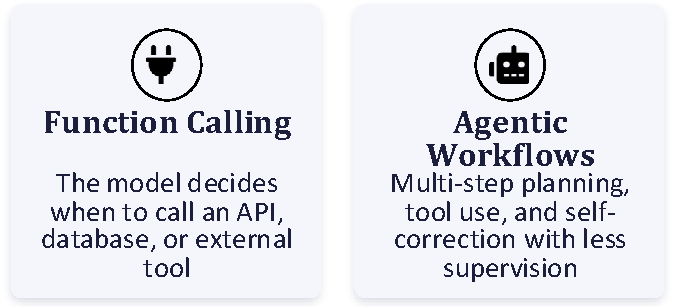
\includegraphics[width=\linewidth,height=3.7cm,keepaspectratio]{images/stanford_agentic_capabilities.pdf}
\par{\fontsize{7}{8.3}\selectfont\color{Slate} Original Stanford figure: one function call and a multi-step workflow.}
\par\endgroup\smallskip
{
\small\begin{itemize}
\setlength{\itemsep}{.25em}
\item A tool does one job. An agent can connect several jobs using their results.
\end{itemize}\par}
\vfill
{\fontsize{6.3}{7.5}\selectfont\color{Slate} Source: \href{https://web.stanford.edu/class/cs224v/lectures_2026/l-introduction.pdf}{Monica Lam. CS224V Agentic AI, Lecture 1: Introduction. Stanford University, Fall 2026, p.2.}\par}
\note{**Say**

A tool does one job. An agent can connect several jobs using their results. A solver can answer a well-defined study request. The agent's job is deciding which permitted request should come next.

**Show**

Use the actual source image. Point to the returned status or number that supports the slide's statement. State whether it is a fresh calculation or a saved example.

**Colab: NO NEW RUN**

Explain the figure or discuss the output already produced. Do not run ahead.

**Ask**

What does the agent add to one tool call?

**Answer**

It can choose and connect permitted next steps using the returned results.

Monica Lam. CS224V Agentic AI, Lecture 1: Introduction. Stanford University. Fall 2026.
Full source: https://web.stan\allowbreak{}ford.edu/class/c\allowbreak{}s224v/lectures\_2\allowbreak{}026/l-introducti\allowbreak{}on.pdf
Publication: https://web.stanford.edu/class/cs224v/

Erik S., Barry Zhang. Building effective agents. Anthropic Engineering. 2024-12-19.
Full source: https://www.anth\allowbreak{}ropic.com/resear\allowbreak{}ch/building-effe\allowbreak{}ctive-agents

Classroom Labs notebook and Python helper. L10B: Watch how Llama chooses a tool; src/llama\_walkthrough.py. Public reproducible teaching material. 24 October 2026.
Full source: https://github.c\allowbreak{}om/AlaaSelim-sud\allowbreak{}o/GridGuard-Agen\allowbreak{}tic-AI-Tutorials\allowbreak{}/blob/main/agent\allowbreak{}ic\_grid\_workflow\allowbreak{}\_tutorial/src/ll\allowbreak{}ama\_walkthrough.\allowbreak{}py}
\end{frame}

\begin{frame}[t]{Solar settings: which option should we try?}
\relax
\begingroup\begin{minipage}[c][3.8cm][c]{\linewidth}\centering\setbox0=\hbox{\resizebox{.96\linewidth}{!}{\begingroup
\begin{tikzpicture}[x=1cm,y=1cm,font=\sffamily\fontsize{10}{12}\selectfont,
every node/.style={text=Navy,align=center},
flow/.style={-{Stealth[length=2.2mm]},draw=IEEEBlue,line width=1.3pt},
box/.style={draw=IEEEBlue,line width=1.1pt,inner sep=7pt,minimum height=.95cm},
small/.style={font=\sffamily\fontsize{8.5}{11}\selectfont}]

\node[text=IEEEBlue,font=\sffamily\bfseries] at (2,4.0) {L2: define the case};
\node[text width=3.4cm] (input) at (2,2.65) {Load case\\Current allowance};
\node[box,text width=3.0cm] (tool) at (6.85,2.65) {Calculate a plan\\Check the current};
\draw[flow] (input)--(tool);
\draw[flow] (tool.east)--(9.35,2.65);
\node[text=IEEEBlue,font=\sffamily\bfseries] at (11.55,4.0) {Read the tool result};
\fill[IEEEBlue] (9.65,2.35) rectangle (12.5948,2.95);
\draw[Red,dashed,line width=1.1pt] (13.65,1.95)--(13.65,3.45);
\node[small,text=Red] at (13.45,3.65) {100\% limit};
\node[small,text=white] at (11.12,2.65) {73.62\%};
\node[small] at (9.65,1.65) {0\%};
\node[small,text width=4.6cm] at (11.65,1.1) {Percent of allowed current\\Reference L2 MPC result};
\node[text=Cyan,text width=13.5cm] at (7.1,.25) {This current check passes. Review voltage and model coverage too.};

\end{tikzpicture}
\endgroup
}}\ifdim\dimexpr\ht0+\dp0\relax>3.8cm\resizebox{!}{3.8cm}{\box0}\else\box0\fi\par\end{minipage}\par
{\fontsize{7}{8.3}\selectfont\color{Slate} Teaching adaptation. L2 runs Python; L10B replays saved model choices.\par}
\endgroup\smallskip
{
\small\begin{itemize}
\setlength{\itemsep}{.25em}
\item Compare possible settings, then check voltage and line current.
\item The agent can organize these trials and report the checked options.
\end{itemize}\par}
\vfill
{\fontsize{6.3}{7.5}\selectfont\color{Slate} Source: \href{https://colab.research.google.com/github/AlaaSelim-sudo/GridGuard-Agentic-AI-Tutorials/blob/main/agentic_grid_workflow_tutorial/Classroom_Labs.ipynb}{Monica Lam. CS224V Agentic AI, Lecture 1: Introduction. Stanford University, Fall 2026, p.19; Classroom Labs L2.}\par}
\note{**Say**

Compare possible settings, then check voltage and line current. The agent can organize these trials and report the checked options. Think of several possible solar settings on the operator's desk. Each candidate needs the same limit checks before comparison.

**Show**

Use the two short slide statements to explain the idea. Link it to the operator's next decision or to the named Colab cell.

**Colab: PREVIEW ONLY**

Show the slide only. Run L2 later on slide 19; keep the notebook in order.

**Expected result**

No new notebook output on this slide.

Monica Lam. CS224V Agentic AI, Lecture 1: Introduction. Stanford University. Fall 2026.
Full source: https://web.stan\allowbreak{}ford.edu/class/c\allowbreak{}s224v/lectures\_2\allowbreak{}026/l-introducti\allowbreak{}on.pdf
Publication: https://web.stanford.edu/class/cs224v/

Sina J. Semnani, Violet Z. Yao, Heidi C. Zhang, Monica S. Lam. WikiChat: Stopping the Hallucination of Large Language Model Chatbots by Few-Shot Grounding on Wikipedia. Findings of the Association for Computational Linguistics: EMNLP 2023, pp.2387--2413. December 2023.
Full source: https://aclantho\allowbreak{}logy.org/2023.fi\allowbreak{}ndings-emnlp.157\allowbreak{}/
Full paper: https://aclantho\allowbreak{}logy.org/2023.fi\allowbreak{}ndings-emnlp.157\allowbreak{}.pdf

Classroom Labs notebook. Classroom\_Labs.ipynb, L2; cell classroom-007; src/continuous\_control.py. Public notebook and Python source. 24 October 2026; stable notebook cell IDs checked.
Full source: https://github.c\allowbreak{}om/AlaaSelim-sud\allowbreak{}o/GridGuard-Agen\allowbreak{}tic-AI-Tutorials\allowbreak{}/blob/main/agent\allowbreak{}ic\_grid\_workflow\allowbreak{}\_tutorial/Classr\allowbreak{}oom\_Labs.ipynb

Classroom Labs notebook and Python helper. L10B: Watch how Llama chooses a tool; src/llama\_walkthrough.py. Public reproducible teaching material. 24 October 2026.
Full source: https://github.c\allowbreak{}om/AlaaSelim-sud\allowbreak{}o/GridGuard-Agen\allowbreak{}tic-AI-Tutorials\allowbreak{}/blob/main/agent\allowbreak{}ic\_grid\_workflow\allowbreak{}\_tutorial/src/ll\allowbreak{}ama\_walkthrough.\allowbreak{}py}
\end{frame}

\begin{frame}[t]{Give the agent a goal and clear limits}
\relax
\begingroup\begin{minipage}[c][3.3cm][c]{\linewidth}\centering\setbox0=\hbox{\resizebox{.96\linewidth}{!}{\definecolor{Red}{HTML}{B83136}
\begin{tikzpicture}[x=1cm,y=1cm,font=\rmfamily\fontsize{12}{14}\selectfont,
 every node/.style={text=Navy,align=center},>=Latex,
 flow/.style={->,draw=IEEEBlue,line width=1.25pt},
 plainpoint/.style={circle,draw=IEEEBlue,fill=white,line width=1.25pt,minimum size=.55cm,inner sep=1pt}]

\node[plainpoint] (s0) at (0.8,1.6) {1};
\node[anchor=north,text width=3.1cm,font=\rmfamily\bfseries\fontsize{12}{14}\selectfont] at (0.8,1.08) {State the goal};
\node[anchor=north,text width=3.1cm,text=Slate,font=\rmfamily\fontsize{11}{13}\selectfont] at (0.8,-.35) {What should be achieved?};
\node[plainpoint] (s1) at (7.3999999999999995,1.6) {2};
\node[anchor=north,text width=3.1cm,font=\rmfamily\bfseries\fontsize{12}{14}\selectfont] at (7.3999999999999995,1.08) {Name allowed tools};
\node[anchor=north,text width=3.1cm,text=Slate,font=\rmfamily\fontsize{11}{13}\selectfont] at (7.3999999999999995,-.35) {What may be requested?};
\draw[flow] (s0)--(s1);
\node[plainpoint] (s2) at (14.0,1.6) {3};
\node[anchor=north,text width=3.1cm,font=\rmfamily\bfseries\fontsize{12}{14}\selectfont] at (14.0,1.08) {Set stop rules};
\node[anchor=north,text width=3.1cm,text=Slate,font=\rmfamily\fontsize{11}{13}\selectfont] at (14.0,-.35) {When is review needed?};
\draw[flow] (s1)--(s2);
\end{tikzpicture}
}}\ifdim\dimexpr\ht0+\dp0\relax>3.3cm\resizebox{!}{3.3cm}{\box0}\else\box0\fi\par\end{minipage}\par
{\fontsize{7}{8.3}\selectfont\color{Slate} Grid teaching adaptation of Stanford's task-specification concept.\par}
\endgroup\smallskip
{
\small\begin{itemize}
\setlength{\itemsep}{.25em}
\item State the goal, allowed tools and stopping rules.
\item Keep the operator's review step explicit.
\end{itemize}\par}
\vfill
{\fontsize{6.3}{7.5}\selectfont\color{Slate} Source: \href{https://web.stanford.edu/class/cs224v/lectures_2026/l-introduction.pdf}{Monica Lam. CS224V Agentic AI, Lecture 1: Introduction. Stanford University, Fall 2026, p.40.}\par}
\note{**Say**

State the goal, allowed tools and stopping rules. Keep the operator's review step explicit. These rules belong to the application and operating process. A persuasive model response cannot change them.

**Show**

Read the visual from the input to the result. Name the operator's goal, the agent's request and the fact supplied by the tool. Explain the decision in the two slide sentences.

**Colab: NO NEW RUN**

Explain the figure or discuss the output already produced. Do not run ahead.

**Ask**

Who sets the limits and allowed actions?

**Answer**

The application and operating process, with the operator's stated task and authority.

Monica Lam. CS224V Agentic AI, Lecture 1: Introduction. Stanford University. Fall 2026.
Full source: https://web.stan\allowbreak{}ford.edu/class/c\allowbreak{}s224v/lectures\_2\allowbreak{}026/l-introducti\allowbreak{}on.pdf
Publication: https://web.stanford.edu/class/cs224v/

Harshit Joshi, Shicheng Liu, James Chen, Larsen Weigle, Monica Lam. Controllable and Reliable Knowledge-Intensive Task-Oriented Conversational Agents with Declarative Genie Worksheets. Proceedings of the 63rd Annual Meeting of the Association for Computational Linguistics, Volume 1: Long Papers, pp.27264--27308. July 2025.
Full source: https://aclanthology.org/2025.acl-long.1323/
Full paper: https://aclantho\allowbreak{}logy.org/2025.ac\allowbreak{}l-long.1323.pdf

Classroom Labs notebook. Classroom\_Labs.ipynb, L0--L1; cells classroom-002 and classroom-004. Public notebook and Python source. 24 October 2026; stable notebook cell IDs checked.
Full source: https://github.c\allowbreak{}om/AlaaSelim-sud\allowbreak{}o/GridGuard-Agen\allowbreak{}tic-AI-Tutorials\allowbreak{}/blob/main/agent\allowbreak{}ic\_grid\_workflow\allowbreak{}\_tutorial/Classr\allowbreak{}oom\_Labs.ipynb}
\end{frame}

\begin{frame}[t]{Restoration: who should get power first?}
\relax
\begingroup\begin{minipage}[c][3.8cm][c]{\linewidth}\centering\setbox0=\hbox{\resizebox{.96\linewidth}{!}{\begingroup
\begin{tikzpicture}[x=1cm,y=1cm,font=\sffamily\fontsize{10}{12}\selectfont,
every node/.style={text=Navy,align=center},
flow/.style={-{Stealth[length=2.2mm]},draw=IEEEBlue,line width=1.3pt},
box/.style={draw=IEEEBlue,line width=1.1pt,inner sep=7pt,minimum height=.95cm},
small/.style={font=\sffamily\fontsize{8.5}{11}\selectfont}]

\node[text=Slate,small] at (7.2,4.0) {L6 / varied tie: 40 kW / fixed tie: 100 kW / totals include upstream load};
\node[text width=4.0cm,align=left,font=\sffamily\bfseries] at (2.2,2.9) {Give critical service\\more weight};
\node[text width=4.0cm,align=left,font=\sffamily\bfseries] at (2.2,1.5) {Serve the most\\total kW};
\fill[Cyan] (5.2,2.55) rectangle (9.7,3.25);
\fill[IEEEBlue] (9.7,2.55) rectangle (11.7,3.25);
\node[text=Navy,font=\sffamily\bfseries] at (7.45,2.9) {90};
\node[text=white,font=\sffamily\bfseries] at (10.7,2.9) {40};
\node[anchor=west] at (12.0,2.9) {130 kW total};
\fill[Cyan] (5.2,1.15) rectangle (6.7,1.85);
\fill[IEEEBlue] (6.7,1.15) rectangle (12.2,1.85);
\node[text=Navy,font=\sffamily\bfseries] at (5.95,1.5) {30};
\node[text=white,font=\sffamily\bfseries] at (9.45,1.5) {110};
\node[anchor=west] at (12.5,1.5) {140 kW total};
\fill[Cyan] (4.1,.25) rectangle (4.5,.6);\node[anchor=west,small] at (4.65,.425) {Critical service};
\fill[IEEEBlue] (8.2,.25) rectangle (8.6,.6);\node[anchor=west,small] at (8.75,.425) {Other service};

\end{tikzpicture}
\endgroup
}}\ifdim\dimexpr\ht0+\dp0\relax>3.8cm\resizebox{!}{3.8cm}{\box0}\else\box0\fi\par\end{minipage}\par
{\fontsize{7}{8.3}\selectfont\color{Slate} L6: same network and limits, different service goals.\par}
\endgroup\smallskip
{
\small\begin{itemize}
\setlength{\itemsep}{.25em}
\item The operator sets the service priority.
\item That priority changes what we ask the restoration tool to do.
\end{itemize}\par}
\vfill
{\fontsize{6.3}{7.5}\selectfont\color{Slate} Source: \href{https://colab.research.google.com/github/AlaaSelim-sudo/GridGuard-Agentic-AI-Tutorials/blob/main/agentic_grid_workflow_tutorial/Classroom_Labs.ipynb}{Monica Lam. CS224V Agentic AI, Lecture 1: Introduction. Stanford University, Fall 2026, p.40; Classroom Labs L6.}\par}
\note{**Say**

The operator sets the service priority. That priority changes what we ask the restoration tool to do. For example, serving more total power can differ from serving more critical demand. The operator must state the intended goal.

**Show**

Use the two short slide statements to explain the idea. Link it to the operator's next decision or to the named Colab cell.

**Colab: PREVIEW ONLY**

Show the slide only. Run L6 later on slide 37; keep the notebook in order.

**Expected result**

No new notebook output on this slide.

Monica Lam. CS224V Agentic AI, Lecture 1: Introduction. Stanford University. Fall 2026.
Full source: https://web.stan\allowbreak{}ford.edu/class/c\allowbreak{}s224v/lectures\_2\allowbreak{}026/l-introducti\allowbreak{}on.pdf
Publication: https://web.stanford.edu/class/cs224v/

Harshit Joshi, Shicheng Liu, James Chen, Larsen Weigle, Monica Lam. Controllable and Reliable Knowledge-Intensive Task-Oriented Conversational Agents with Declarative Genie Worksheets. Proceedings of the 63rd Annual Meeting of the Association for Computational Linguistics, Volume 1: Long Papers, pp.27264--27308. July 2025.
Full source: https://aclanthology.org/2025.acl-long.1323/
Full paper: https://aclantho\allowbreak{}logy.org/2025.ac\allowbreak{}l-long.1323.pdf

Classroom Labs notebook. Classroom\_Labs.ipynb, L6; cell classroom-018; src/standard\_formulations.py. Public notebook and Python source. 24 October 2026; stable notebook cell IDs checked.
Full source: https://github.c\allowbreak{}om/AlaaSelim-sud\allowbreak{}o/GridGuard-Agen\allowbreak{}tic-AI-Tutorials\allowbreak{}/blob/main/agent\allowbreak{}ic\_grid\_workflow\allowbreak{}\_tutorial/Classr\allowbreak{}oom\_Labs.ipynb

Classroom Labs notebook and Python helper. L10B: Watch how Llama chooses a tool; src/llama\_walkthrough.py. Public reproducible teaching material. 24 October 2026.
Full source: https://github.c\allowbreak{}om/AlaaSelim-sud\allowbreak{}o/GridGuard-Agen\allowbreak{}tic-AI-Tutorials\allowbreak{}/blob/main/agent\allowbreak{}ic\_grid\_workflow\allowbreak{}\_tutorial/src/ll\allowbreak{}ama\_walkthrough.\allowbreak{}py}
\end{frame}

\begin{frame}[t]{Keep three jobs clear}
\relax
\begingroup\begin{minipage}[c][3.3cm][c]{\linewidth}\centering\setbox0=\hbox{\resizebox{.96\linewidth}{!}{\definecolor{Red}{HTML}{B83136}
\begin{tikzpicture}[x=1cm,y=1cm,font=\rmfamily\fontsize{12}{14}\selectfont,
 every node/.style={text=Navy,align=center},>=Latex,
 flow/.style={->,draw=IEEEBlue,line width=1.25pt},
 plainpoint/.style={circle,draw=IEEEBlue,fill=white,line width=1.25pt,minimum size=.55cm,inner sep=1pt}]

\node[plainpoint] (s0) at (0.8,1.6) {1};
\node[anchor=north,text width=3.1cm,font=\rmfamily\bfseries\fontsize{12}{14}\selectfont] at (0.8,1.08) {Agent requests};
\node[anchor=north,text width=3.1cm,text=Slate,font=\rmfamily\fontsize{11}{13}\selectfont] at (0.8,-.35) {Choose the study};
\node[plainpoint] (s1) at (7.3999999999999995,1.6) {2};
\node[anchor=north,text width=3.1cm,font=\rmfamily\bfseries\fontsize{12}{14}\selectfont] at (7.3999999999999995,1.08) {Tool calculates};
\node[anchor=north,text width=3.1cm,text=Slate,font=\rmfamily\fontsize{11}{13}\selectfont] at (7.3999999999999995,-.35) {Return the result};
\draw[flow] (s0)--(s1);
\node[plainpoint] (s2) at (14.0,1.6) {3};
\node[anchor=north,text width=3.1cm,font=\rmfamily\bfseries\fontsize{12}{14}\selectfont] at (14.0,1.08) {Operator decides};
\node[anchor=north,text width=3.1cm,text=Slate,font=\rmfamily\fontsize{11}{13}\selectfont] at (14.0,-.35) {Review the next step};
\draw[flow] (s1)--(s2);
\end{tikzpicture}
}}\ifdim\dimexpr\ht0+\dp0\relax>3.3cm\resizebox{!}{3.3cm}{\box0}\else\box0\fi\par\end{minipage}\par
{\fontsize{7}{8.3}\selectfont\color{Slate} Adapted principle: language, calculation and human review have different jobs.\par}
\endgroup\smallskip
{
\small\begin{itemize}
\setlength{\itemsep}{.25em}
\item The agent requests a study. The tool calculates. The operator reviews the result.
\end{itemize}\par}
\vfill
{\fontsize{6.3}{7.5}\selectfont\color{Slate} Source: \href{https://colab.research.google.com/github/AlaaSelim-sudo/GridGuard-Agentic-AI-Tutorials/blob/main/agentic_grid_workflow_tutorial/Classroom_Labs.ipynb}{Monica Lam. CS224V Agentic AI, Lecture 1: Introduction. Stanford University, Fall 2026, p.53.}\par}
\note{**Say**

The agent requests a study. The tool calculates. The operator reviews the result. Keep the three responsibilities separate when reading the examples. A fluent explanation is not a substitute for the calculation.

**Show**

Read the visual from the input to the result. Name the operator's goal, the agent's request and the fact supplied by the tool. Explain the decision in the two slide sentences.

**Colab: NO NEW RUN**

Explain the figure or discuss the output already produced. Do not run ahead.

**Ask**

Which job belongs to the operator?

**Answer**

Reviewing the evidence and deciding the next authorized step.

Monica Lam. CS224V Agentic AI, Lecture 1: Introduction. Stanford University. Fall 2026.
Full source: https://web.stan\allowbreak{}ford.edu/class/c\allowbreak{}s224v/lectures\_2\allowbreak{}026/l-introducti\allowbreak{}on.pdf
Publication: https://web.stanford.edu/class/cs224v/

Classroom Labs notebook. Classroom\_Labs.ipynb, L9; cell classroom-026; fixed trusted-recovery fixture. Public notebook and Python source. 24 October 2026; stable notebook cell IDs checked.
Full source: https://github.c\allowbreak{}om/AlaaSelim-sud\allowbreak{}o/GridGuard-Agen\allowbreak{}tic-AI-Tutorials\allowbreak{}/blob/main/agent\allowbreak{}ic\_grid\_workflow\allowbreak{}\_tutorial/Classr\allowbreak{}oom\_Labs.ipynb}
\end{frame}

\begin{frame}[t]{Wrong readings can still fit a model}
\relax
\begingroup\begin{minipage}[c][3.8cm][c]{\linewidth}\centering\setbox0=\hbox{\resizebox{.96\linewidth}{!}{\begingroup
\begin{tikzpicture}[x=1cm,y=1cm,font=\sffamily\fontsize{10}{12}\selectfont,
every node/.style={text=Navy,align=center},
flow/.style={-{Stealth[length=2.2mm]},draw=IEEEBlue,line width=1.3pt},
box/.style={draw=IEEEBlue,line width=1.1pt,inner sep=7pt,minimum height=.95cm},
small/.style={font=\sffamily\fontsize{8.5}{11}\selectfont}]

\node[anchor=west,text=IEEEBlue,font=\sffamily\bfseries] at (.2,4.35) {L8: do the readings fit the model?};
\node[text width=2.4cm] (data) at (1.65,3.5) {Readings};
\node[box,text width=3.4cm] (fit) at (7.2,3.5) {Python fits the model};
\node[text width=3.6cm] (res) at (12.6,3.5) {Small mismatch\\can still hide an error};
\draw[flow] (data)--(fit);\draw[flow] (fit)--(res);
\draw[Slate!35] (.2,2.6)--(14.4,2.6);
\node[anchor=west,text=IEEEBlue,font=\sffamily\bfseries] at (.2,2.2) {L9: is recovery supported?};
\node[text width=5.5cm] (trust) at (7.2,1.3) {Trusted data assumed\\and recovery check passes?};
\node[draw=Red,text=Red,inner sep=7pt,line width=1.1pt] (hold) at (1.6,1.3) {HOLD};
\node[draw=Cyan,text=Cyan,inner sep=7pt,line width=1.1pt] (propose) at (12.8,1.3) {PROPOSE};
\draw[flow] (trust.west)--node[above,small]{No}(hold.east);
\draw[flow] (trust.east)--node[above,small]{Yes}(propose.west);
\node[small,text=Slate,text width=14cm] at (7.2,.2) {L9 assumes those extra readings are trusted. The numerical tool does not authenticate them.};

\end{tikzpicture}
\endgroup
}}\ifdim\dimexpr\ht0+\dp0\relax>3.8cm\resizebox{!}{3.8cm}{\box0}\else\box0\fi\par\end{minipage}\par
{\fontsize{7}{8.3}\selectfont\color{Slate} L8 checks fit. L9 requires a trust assumption before proposing recovery.\par}
\endgroup\smallskip
{
\small\begin{itemize}
\setlength{\itemsep}{.25em}
\item A good fit alone does not prove the readings are true.
\item The agent can organize checks and flag missing evidence.
\end{itemize}\par}
\vfill
{\fontsize{6.3}{7.5}\selectfont\color{Slate} Source: \href{https://colab.research.google.com/github/AlaaSelim-sudo/GridGuard-Agentic-AI-Tutorials/blob/main/agentic_grid_workflow_tutorial/Classroom_Labs.ipynb}{Monica Lam. CS224V Agentic AI, Lecture 1: Introduction. Stanford University, Fall 2026, p.53; Classroom Labs L8--L9.}\par}
\note{**Say**

A good fit alone does not prove the readings are true. The agent can organize checks and flag missing evidence. Later we will change readings in a small model and compare the alarm with the resulting estimation error.

**Show**

Use the two short slide statements to explain the idea. Link it to the operator's next decision or to the named Colab cell.

**Colab: PREVIEW ONLY**

Show the slide only. Run L8 later on slide 51; keep the notebook in order.

**Expected result**

No new notebook output on this slide.

Monica Lam. CS224V Agentic AI, Lecture 1: Introduction. Stanford University. Fall 2026.
Full source: https://web.stan\allowbreak{}ford.edu/class/c\allowbreak{}s224v/lectures\_2\allowbreak{}026/l-introducti\allowbreak{}on.pdf
Publication: https://web.stanford.edu/class/cs224v/

Classroom Labs notebook. Classroom\_Labs.ipynb, L8; cell classroom-023; four-bus DC fixture. Public notebook and Python source. 24 October 2026; stable notebook cell IDs checked.
Full source: https://github.c\allowbreak{}om/AlaaSelim-sud\allowbreak{}o/GridGuard-Agen\allowbreak{}tic-AI-Tutorials\allowbreak{}/blob/main/agent\allowbreak{}ic\_grid\_workflow\allowbreak{}\_tutorial/Classr\allowbreak{}oom\_Labs.ipynb

Classroom Labs notebook. Classroom\_Labs.ipynb, L9; cell classroom-026; fixed trusted-recovery fixture. Public notebook and Python source. 24 October 2026; stable notebook cell IDs checked.
Full source: https://github.c\allowbreak{}om/AlaaSelim-sud\allowbreak{}o/GridGuard-Agen\allowbreak{}tic-AI-Tutorials\allowbreak{}/blob/main/agent\allowbreak{}ic\_grid\_workflow\allowbreak{}\_tutorial/Classr\allowbreak{}oom\_Labs.ipynb

Classroom Labs notebook and Python helper. L10B: Watch how Llama chooses a tool; src/llama\_walkthrough.py. Public reproducible teaching material. 24 October 2026.
Full source: https://github.c\allowbreak{}om/AlaaSelim-sud\allowbreak{}o/GridGuard-Agen\allowbreak{}tic-AI-Tutorials\allowbreak{}/blob/main/agent\allowbreak{}ic\_grid\_workflow\allowbreak{}\_tutorial/src/ll\allowbreak{}ama\_walkthrough.\allowbreak{}py}
\end{frame}

\begin{frame}[t]{Use one notebook for all three cases}
\relax
\begingroup\begin{minipage}[c][3.5cm][c]{\linewidth}\centering\setbox0=\hbox{\resizebox{.96\linewidth}{!}{\begingroup
\begin{tikzpicture}[x=1cm,y=1cm,font=\sffamily\fontsize{9.5}{12}\selectfont,
every node/.style={text=Navy,align=center},
flow/.style={-{Stealth[length=2mm]},draw=IEEEBlue,line width=1.2pt},
label/.style={text width=2.5cm,align=center},
box/.style={draw=IEEEBlue,line width=1pt,fill=white,inner sep=7pt,minimum height=1cm},
small/.style={font=\sffamily\fontsize{8}{10}\selectfont},
stop/.style={draw=Red,text=Red,fill=Red!4,line width=1pt,inner sep=6pt}]
\path[use as bounding box] (-.05,-.1) rectangle (14.5,4.0);

\node[box,text width=5.1cm,font=\ttfamily\fontsize{10}{12}\selectfont] (book) at (7.2,3.2) {Classroom\_Labs.ipynb};
\node[text=IEEEBlue,text width=3.4cm] (v) at (2.3,1.7) {Voltage\\L2--L5};
\node[text=IEEEBlue,text width=3.4cm] (r) at (7.2,1.7) {Restoration\\L6--L7};
\node[text=IEEEBlue,text width=3.4cm] (c) at (12.1,1.7) {Cyber\\L8--L9};
\draw[flow] (book.south)--(7.2,2.5)-|(v.north);\draw[flow] (book.south)--(r.north);\draw[flow] (7.2,2.5)-|(c.north);
\node[small,text width=4.3cm] at (2.3,.75) {Change a current allowance};
\node[small,text width=4.3cm] at (7.2,.75) {Change a tie capacity};
\node[small,text width=4.3cm] at (12.1,.75) {Change a data bias};
\node[small,text=Slate] at (7.2,.05) {L10B replays Llama choices in the same file. Each case uses a separate teaching network.};

\end{tikzpicture}
\endgroup
}}\ifdim\dimexpr\ht0+\dp0\relax>3.5cm\resizebox{!}{3.5cm}{\box0}\else\box0\fi\par\end{minipage}\par
{\fontsize{7}{8.3}\selectfont\color{Slate} Classroom Labs is the only required notebook.\par}
\endgroup\smallskip
{\large\color{IEEEBlue} \href{https://colab.research.google.com/github/AlaaSelim-sudo/GridGuard-Agentic-AI-Tutorials/blob/main/agentic_grid_workflow_tutorial/Classroom_Labs.ipynb}{Open Classroom Labs in Google Colab}\par}\medskip
{
\small\begin{itemize}
\setlength{\itemsep}{.25em}
\item Open Classroom Labs and save your own copy.
\item We will use it throughout the workshop.
\end{itemize}\par}
\vfill
{\fontsize{6.3}{7.5}\selectfont\color{Slate} Source: \href{https://colab.research.google.com/github/AlaaSelim-sudo/GridGuard-Agentic-AI-Tutorials/blob/main/agentic_grid_workflow_tutorial/Classroom_Labs.ipynb}{Setup: COLAB\_GUIDE.md; Classroom\_Labs.ipynb.}\par}
\note{**Say**

Open Classroom Labs and save your own copy. We will use it throughout the workshop. Other notebooks on the website are supporting resources. Classroom Labs is the one required notebook for this session.

**Show**

Use the two short slide statements to explain the idea. Link it to the operator's next decision or to the named Colab cell.

**Colab: NO NEW RUN**

Open Classroom Labs and save a copy. Run setup on slide 10, not the later lesson cells.

Classroom Labs notebook. Setup: COLAB\_GUIDE.md; Classroom\_Labs.ipynb. Public notebook and Python source. 24 October 2026; stable notebook cell IDs checked.
Full source: https://github.c\allowbreak{}om/AlaaSelim-sud\allowbreak{}o/GridGuard-Agen\allowbreak{}tic-AI-Tutorials\allowbreak{}/blob/main/COLAB\allowbreak{}\_GUIDE.md}
\end{frame}

\begin{frame}[t]{Start Colab in three steps}
\relax
\begingroup\begin{minipage}[c][3.3cm][c]{\linewidth}\centering\setbox0=\hbox{\resizebox{.96\linewidth}{!}{\begingroup
\begin{tikzpicture}[x=1cm,y=1cm,font=\sffamily\fontsize{9.5}{12}\selectfont,
every node/.style={text=Navy,align=center},
flow/.style={-{Stealth[length=2mm]},draw=IEEEBlue,line width=1.2pt},
label/.style={text width=2.5cm,align=center},
box/.style={draw=IEEEBlue,line width=1pt,fill=white,inner sep=7pt,minimum height=1cm},
small/.style={font=\sffamily\fontsize{8}{10}\selectfont},
stop/.style={draw=Red,text=Red,fill=Red!4,line width=1pt,inner sep=6pt}]
\path[use as bounding box] (-.05,-.1) rectangle (14.5,4.0);

\foreach \x/\n/\t/\d in {1.6/1/Open/Use the Colab link,5.3/2/Keep/Save a Drive copy,9.0/3/Connect/CPU runtime,12.7/4/Prepare/Run setup to Ready} {
\node[circle,draw=IEEEBlue,line width=1pt,minimum size=.7cm] at (\x,2.7) {\n};
\node[text=IEEEBlue] at (\x,1.95) {\t};\node[small,text width=3.0cm] at (\x,1.2) {\d};}
\foreach \a/\b in {2.1/4.8,5.8/8.5,9.5/12.2}{\draw[flow] (\a,2.7)--(\b,2.7);}
\node[text=Slate,small,text width=13.7cm] at (7.2,.25) {For the guided workshop, run each named lesson when prompted. Run all is a useful setup check.};

\end{tikzpicture}
\endgroup
}}\ifdim\dimexpr\ht0+\dp0\relax>3.3cm\resizebox{!}{3.3cm}{\box0}\else\box0\fi\par\end{minipage}\par
{\fontsize{7}{8.3}\selectfont\color{Slate} Setup first, then L0 and L1.\par}
\endgroup\smallskip
{
\small\begin{itemize}
\setlength{\itemsep}{.25em}
\item Save a copy, connect a CPU and run setup.
\item Wait for Ready, then run L0 and L1.
\end{itemize}\par}
\vfill
{\fontsize{6.3}{7.5}\selectfont\color{Slate} Source: \href{https://colab.research.google.com/github/AlaaSelim-sudo/GridGuard-Agentic-AI-Tutorials/blob/main/agentic_grid_workflow_tutorial/Classroom_Labs.ipynb}{Setup: COLAB\_GUIDE.md; Classroom\_Labs.ipynb.}\par}
\note{**Say**

Save a copy, connect a CPU and run setup. Wait for Ready, then run L0 and L1. Colab gives you a temporary computer. After a runtime reset, rerun setup and the earlier cells to recreate their variables.

**Show**

Use the two short slide statements to explain the idea. Link it to the operator's next decision or to the named Colab cell.

**Colab: RUN**

Connect a CPU. Run the whole setup cell once and wait for Ready.

Exact cells: colab-setup. Run the whole cell, not only the slide excerpt.

**Expected result**

Ready appears; the support files and CPU packages are available.

Classroom Labs notebook. Setup: COLAB\_GUIDE.md; Classroom\_Labs.ipynb. Public notebook and Python source. 24 October 2026; stable notebook cell IDs checked.
Full source: https://github.c\allowbreak{}om/AlaaSelim-sud\allowbreak{}o/GridGuard-Agen\allowbreak{}tic-AI-Tutorials\allowbreak{}/blob/main/COLAB\allowbreak{}\_GUIDE.md

Google Colaboratory. Frequently Asked Questions: Using Colab, notebook storage and execution state. Google Research. Reviewed 24 October 2026.
Full source: https://research\allowbreak{}.google.com/cola\allowbreak{}boratory/faq.htm\allowbreak{}l}
\end{frame}

\begin{frame}[t]{Run a cell, then read its output}
\relax
\begingroup\begin{minipage}[c][3.5cm][c]{\linewidth}\centering\setbox0=\hbox{\resizebox{.96\linewidth}{!}{\begingroup
\begin{tikzpicture}[x=1cm,y=1cm,font=\sffamily\fontsize{9.5}{12}\selectfont,
every node/.style={text=Navy,align=center},
flow/.style={-{Stealth[length=2mm]},draw=IEEEBlue,line width=1.2pt},
label/.style={text width=2.5cm,align=center},
box/.style={draw=IEEEBlue,line width=1pt,fill=white,inner sep=7pt,minimum height=1cm},
small/.style={font=\sffamily\fontsize{8}{10}\selectfont},
stop/.style={draw=Red,text=Red,fill=Red!4,line width=1pt,inner sep=6pt}]
\path[use as bounding box] (-.05,-.1) rectangle (14.5,4.0);

\node[text=IEEEBlue,font=\sffamily\bfseries] at (2.7,3.55) {1. Input};
\node[box,text width=4.5cm,font=\ttfamily\fontsize{9}{12}\selectfont] (code) at (2.7,2.0) {LOAD\_SCALE = 1.0\\RATING\_FRACTION = 0.80};
\node[text=IEEEBlue] at (7.2,3.55) {2. Run the whole cell};
\draw[IEEEBlue,fill=Cyan!10,line width=1.2pt] (7.2,2.0) circle (.65);
\fill[IEEEBlue] (6.98,1.67)--(6.98,2.33)--(7.51,2.0)--cycle;
\node[box,text width=3.4cm] (result) at (12.2,2.0) {Table + plot\\Read the limit check};
\node[text=IEEEBlue,font=\sffamily\bfseries] at (12.2,3.55) {3. Read the output};
\draw[flow] (code.east)--(6.5,2);\draw[flow] (7.9,2)--(result.west);
\node[small,text=Slate,text width=13cm] at (7.2,.5) {The play button executes Python. The saved text below a cell is its output.};

\end{tikzpicture}
\endgroup
}}\ifdim\dimexpr\ht0+\dp0\relax>3.5cm\resizebox{!}{3.5cm}{\box0}\else\box0\fi\par\end{minipage}\par
{\fontsize{7}{8.3}\selectfont\color{Slate} Illustration of a code cell. Run the full L2 cell.\par}
\endgroup\smallskip
{
\small\begin{itemize}
\setlength{\itemsep}{.25em}
\item Find the L heading and run the whole cell.
\item After changing an input, run that cell again.
\end{itemize}\par}
\vfill
{\fontsize{6.3}{7.5}\selectfont\color{Slate} Source: \href{https://research.google.com/colaboratory/faq.html}{Google Colab FAQ; Classroom Labs L2, cell classroom-007.}\par}
\note{**Say**

Find the L heading and run the whole cell. After changing an input, run that cell again. The play button runs the cell. The output below it belongs to the last completed run, so an edit alone changes nothing.

**Show**

Use the two short slide statements to explain the idea. Link it to the operator's next decision or to the named Colab cell.

**Colab: PREVIEW ONLY**

Show the slide only. Run L2 later on slide 19; keep the notebook in order.

**Expected result**

No new notebook output on this slide.

Google Colaboratory. Frequently Asked Questions: Using Colab, notebook storage and execution state. Google Research. Reviewed 24 October 2026.
Full source: https://research\allowbreak{}.google.com/cola\allowbreak{}boratory/faq.htm\allowbreak{}l

Classroom Labs notebook. Classroom\_Labs.ipynb, L2; cell classroom-007; src/continuous\_control.py. Public notebook and Python source. 24 October 2026; stable notebook cell IDs checked.
Full source: https://github.c\allowbreak{}om/AlaaSelim-sud\allowbreak{}o/GridGuard-Agen\allowbreak{}tic-AI-Tutorials\allowbreak{}/blob/main/agent\allowbreak{}ic\_grid\_workflow\allowbreak{}\_tutorial/Classr\allowbreak{}oom\_Labs.ipynb}
\end{frame}

\begin{frame}[t]{Python runs the default lab}
\relax
{\fontsize{8}{10}\selectfont\color{Slate} Run the whole cell in Colab\par}\smallskip
\lstinputlisting[basicstyle=\ttfamily\fontsize{12}{14.5}\selectfont,aboveskip=3pt,belowskip=10pt,breaklines=true,gobble=0]{../research/code/opening_Classroom_Labs_classroom-002_L11-12.py}
{
\small\begin{itemize}
\setlength{\itemsep}{.25em}
\item In Colab, run L0 with both switches False. Python runs the calculations.
\item The Llama examples use saved replies. No live model is needed.
\end{itemize}\par}
\vfill
{\fontsize{6.3}{7.5}\selectfont\color{Slate} Source: \href{https://colab.research.google.com/github/AlaaSelim-sudo/GridGuard-Agentic-AI-Tutorials/blob/main/agentic_grid_workflow_tutorial/Classroom_Labs.ipynb}{Classroom\_Labs.ipynb, L0--L1; cells classroom-002 and classroom-004.}\par}
\note{**Say**

In Colab, run L0 with both switches False. Python runs the calculations. The Llama examples use saved replies. No live model is needed.

**Show**

Locate L0 in Classroom Labs. Show the highlighted source lines, then run the whole cell when the Colab cue says to run. Read the returned result in plain words.

**Colab: RUN**

Run L0 with RUN\_OPENDSS=False and RUN\_LOCAL\_LLAMA=False.

Exact cells: classroom-002. Run the whole cell, not only the slide excerpt.

**Expected result**

The data assertion passes. Both optional live-tool paths remain off.

Classroom Labs notebook. Classroom\_Labs.ipynb, L0--L1; cells classroom-002 and classroom-004. Public notebook and Python source. 24 October 2026; stable notebook cell IDs checked.
Full source: https://github.c\allowbreak{}om/AlaaSelim-sud\allowbreak{}o/GridGuard-Agen\allowbreak{}tic-AI-Tutorials\allowbreak{}/blob/main/agent\allowbreak{}ic\_grid\_workflow\allowbreak{}\_tutorial/Classr\allowbreak{}oom\_Labs.ipynb}
\end{frame}

\begin{frame}[t]{Does the saved result still match?}
\relax
\begingroup\centering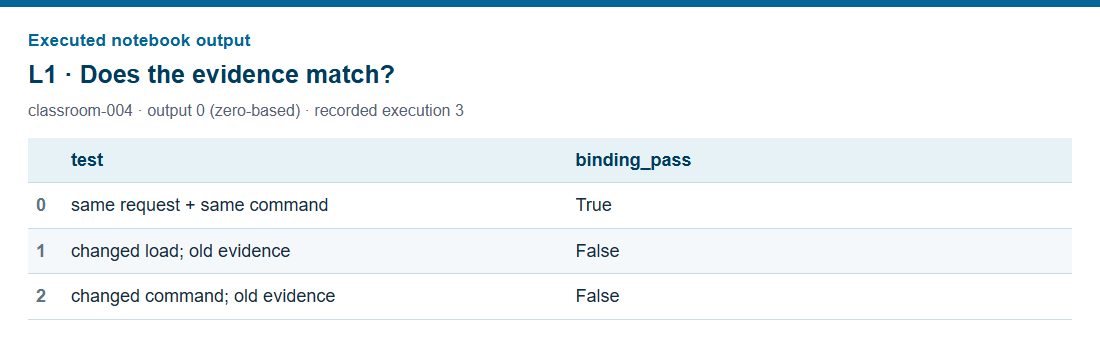
\includegraphics[width=\linewidth,height=3.65cm,keepaspectratio]{images/hands_on_L1_binding.png}
\par{\fontsize{7}{8.3}\selectfont\color{Slate} Reference L1 output. Only the unchanged request and command match.}
\par\endgroup\smallskip
{
\small\begin{itemize}
\setlength{\itemsep}{.25em}
\item Run L1. Only the unchanged request should match its saved result.
\item Changed inputs or actions need a new check.
\end{itemize}\par}
\vfill
{\fontsize{6.3}{7.5}\selectfont\color{Slate} Source: \href{https://colab.research.google.com/github/AlaaSelim-sudo/GridGuard-Agentic-AI-Tutorials/blob/main/agentic_grid_workflow_tutorial/Classroom_Labs.ipynb}{Classroom\_Labs.ipynb, L0--L1; cells classroom-002 and classroom-004.}\par}
\note{**Say**

Run L1. Only the unchanged request should match its saved result. Changed inputs or actions need a new check.

**Show**

Use the actual source image. Point to the returned status or number that supports the slide's statement. State whether it is a fresh calculation or a saved example.

**Colab: RUN**

Run the whole L1 cell after L0.

Exact cells: classroom-004. Run the whole cell, not only the slide excerpt.

**Expected result**

binding\_pass is True, False, False in row order.

Classroom Labs notebook. Classroom\_Labs.ipynb, L0--L1; cells classroom-002 and classroom-004. Public notebook and Python source. 24 October 2026; stable notebook cell IDs checked.
Full source: https://github.c\allowbreak{}om/AlaaSelim-sud\allowbreak{}o/GridGuard-Agen\allowbreak{}tic-AI-Tutorials\allowbreak{}/blob/main/agent\allowbreak{}ic\_grid\_workflow\allowbreak{}\_tutorial/Classr\allowbreak{}oom\_Labs.ipynb}
\end{frame}

\begin{frame}[t]{Case 1: which solar settings should we use?}
\relax
\begingroup\begin{minipage}[c][3.3cm][c]{\linewidth}\centering\setbox0=\hbox{\resizebox{.96\linewidth}{!}{\definecolor{Red}{HTML}{B83136}
\begin{tikzpicture}[x=1cm,y=1cm,font=\rmfamily\fontsize{12}{14}\selectfont,
 every node/.style={text=Navy,align=center},>=Latex,
 flow/.style={->,draw=IEEEBlue,line width=1.25pt},
 plainpoint/.style={circle,draw=IEEEBlue,fill=white,line width=1.25pt,minimum size=.55cm,inner sep=1pt}]

\node[plainpoint] (source) at (.6,1.1) {};
\node[below=.25cm of source] {Supply};
\draw[line width=1.3pt,IEEEBlue] (source.east)--(12,1.1);
\draw[IEEEBlue,line width=1.2pt] (4,2.7) rectangle (6,3.5);
\foreach \x in {4.5,5,5.5}{\draw[Cyan] (\x,2.7)--(\x,3.5);}
\draw[Cyan] (4,3.1)--(6,3.1);
\node at (5,4) {Solar settings};
\draw[flow] (5,2.7)--(5,1.1);
\draw[IEEEBlue] (2.9,3.5) circle (.23);
\foreach \a in {0,45,...,315}{\draw[Cyan] (2.9,3.5)++(\a:.32)--++(\a:.16);}
\node[plainpoint] at (8.2,1.1) {?};
\node[above,text width=3.4cm] at (8.2,1.65) {Voltage and\\line current};
\draw[IEEEBlue,line width=1.2pt] (12,1.1) rectangle (13.5,2);
\draw[IEEEBlue,line width=1.2pt] (11.8,2)--(12.75,2.75)--(13.7,2);
\node at (12.75,.55) {Loads};
\node[text=Slate] at (6.9,-.15) {Choose settings, then check their effects};

\end{tikzpicture}
}}\ifdim\dimexpr\ht0+\dp0\relax>3.3cm\resizebox{!}{3.3cm}{\box0}\else\box0\fi\par\end{minipage}\par
{\fontsize{7}{8.3}\selectfont\color{Slate} Concept sketch. First run the tools; later replay saved agent decisions.\par}
\endgroup\smallskip
{
\small\begin{itemize}
\setlength{\itemsep}{.25em}
\item Choose settings that keep voltage and line current within the allowed range.
\item An agent can organize the trials and return checked options.
\end{itemize}\par}
\vfill
{\fontsize{6.3}{7.5}\selectfont\color{Slate} Source: \href{https://colab.research.google.com/github/AlaaSelim-sudo/GridGuard-Agentic-AI-Tutorials/blob/main/agentic_grid_workflow_tutorial/Classroom_Labs.ipynb}{Classroom\_Labs.ipynb, L2; cell classroom-007; src/continuous\_control.py.}\par}
\note{**Say**

Imagine an operator comparing possible settings for solar units. Each choice changes power flows. The job is to find an acceptable option while respecting voltage, line-current and unit limits. An agent can organize the requests and responses, while the tool calculates the electrical effects. We first learn those tools in Colab, then inspect saved agent decisions.

**Show**

Read the visual from the input to the result. Name the operator's goal, the agent's request and the fact supplied by the tool. Explain the decision in the two slide sentences.

**Colab: PREVIEW ONLY**

Show the slide only. Run L2 later on slide 19; keep the notebook in order.

**Expected result**

No new notebook output on this slide.

**Ask**

What must a proposed solar setting respect?

**Answer**

The checked voltage, line-current and solar-unit limits for the stated model.

Classroom Labs notebook. Classroom\_Labs.ipynb, L2; cell classroom-007; src/continuous\_control.py. Public notebook and Python source. 24 October 2026; stable notebook cell IDs checked.
Full source: https://github.c\allowbreak{}om/AlaaSelim-sud\allowbreak{}o/GridGuard-Agen\allowbreak{}tic-AI-Tutorials\allowbreak{}/blob/main/agent\allowbreak{}ic\_grid\_workflow\allowbreak{}\_tutorial/Classr\allowbreak{}oom\_Labs.ipynb

Existing GridGuard workshop / SMART-DS synthetic-feeder extraction. Synthetic Greensboro feeder uhs20\_1247--udt8894: model map and declared study scope. Existing teaching snapshot reviewed 18 October 2026.
Full source: https://data.openei.org/submissions/2981}
\end{frame}

\begin{frame}[t]{Two tools suggest different settings}
\relax
\begingroup\begin{minipage}[c][3.3cm][c]{\linewidth}\centering\setbox0=\hbox{\resizebox{.96\linewidth}{!}{\definecolor{Red}{HTML}{B83136}
\begin{tikzpicture}[x=1cm,y=1cm,font=\rmfamily\fontsize{12}{14}\selectfont,
 every node/.style={text=Navy,align=center},>=Latex,
 flow/.style={->,draw=IEEEBlue,line width=1.25pt},
 plainpoint/.style={circle,draw=IEEEBlue,fill=white,line width=1.25pt,minimum size=.55cm,inner sep=1pt}]

\node[plainpoint] (a) at (2.5,2.5) {1};\node[above=.25cm of a,font=\rmfamily\bfseries] {MPC};
\node[text width=4cm,below=.25cm of a] {Plan with a model};
\node[plainpoint] (b) at (11,2.5) {2};\node[above=.25cm of b,font=\rmfamily\bfseries] {Saved SAC};
\node[text width=4cm,below=.25cm of b] {Use a learned controller};
\node[plainpoint] (c) at (6.75,.1) {?};
\draw[flow] (a.west)--++(-.8,0)|-(c.west);
\draw[flow] (b.east)--++(.8,0)|-(c.east);
\node[below=.25cm of c,text width=8cm,font=\rmfamily\bfseries] {Same voltage and current checks\\plus equipment capacity};

\end{tikzpicture}
}}\ifdim\dimexpr\ht0+\dp0\relax>3.3cm\resizebox{!}{3.3cm}{\box0}\else\box0\fi\par\end{minipage}\par
{\fontsize{7}{8.3}\selectfont\color{Slate} MPC: model predictive control. SAC: soft actor-critic. Both proposals need the same checks.\par}
\endgroup\smallskip
{
\small\begin{itemize}
\setlength{\itemsep}{.25em}
\item MPC plans with a model. SAC uses a previously trained controller.
\item Treat both outputs as proposals that need the same electrical checks.
\end{itemize}\par}
\vfill
{\fontsize{6.3}{7.5}\selectfont\color{Slate} Source: \href{https://github.com/AlaaSelim-sudo/GridGuard-Agentic-AI-Tutorials/blob/main/agentic_grid_workflow_tutorial/Classroom_Labs.ipynb}{Classroom Labs notebook. Classroom\_Labs.ipynb, L2; cell classroom-007; src/continuous\_control.py. Public notebook and Python source. 24 October 2026; stable notebook cell IDs checked.}\par}
\note{**Say**

MPC plans with a model. SAC uses a previously trained controller. Treat both outputs as proposals that need the same electrical checks. MPC means model predictive control. SAC means soft actor-critic, a learned controller. You do not need their algorithms to follow this lab: both simply supply settings for the same check.

**Show**

Read the visual from the input to the result. Name the operator's goal, the agent's request and the fact supplied by the tool. Explain the decision in the two slide sentences.

**Colab: NO NEW RUN**

Explain the figure or discuss the output already produced. Do not run ahead.

Classroom Labs notebook. Classroom\_Labs.ipynb, L2; cell classroom-007; src/continuous\_control.py. Public notebook and Python source. 24 October 2026; stable notebook cell IDs checked.
Full source: https://github.c\allowbreak{}om/AlaaSelim-sud\allowbreak{}o/GridGuard-Agen\allowbreak{}tic-AI-Tutorials\allowbreak{}/blob/main/agent\allowbreak{}ic\_grid\_workflow\allowbreak{}\_tutorial/Classr\allowbreak{}oom\_Labs.ipynb

James B. Rawlings; David Q. Mayne; Moritz M. Diehl. Model Predictive Control: Theory, Computation, and Design, second edition. Nob Hill Publishing. 2017.
Full source: https://sites.en\allowbreak{}gineering.ucsb.e\allowbreak{}du/\textasciitilde{}jbraw/mpc/MP\allowbreak{}C-book-2nd-editi\allowbreak{}on-1st-printing.\allowbreak{}pdf

Tuomas Haarnoja; Aurick Zhou; Pieter Abbeel; Sergey Levine. Soft Actor-Critic: Off-Policy Maximum Entropy Deep Reinforcement Learning with a Stochastic Actor. Proceedings of the 35th International Conference on Machine Learning, PMLR 80, pp. 1861--1870. 2018.
Full source: https://proceedi\allowbreak{}ngs.mlr.press/v8\allowbreak{}0/haarnoja18b.ht\allowbreak{}ml

Workshop recorded model replies and numerical study records. Voltage P3\_current\_reserve: Llama 3.1:8b planner, recovery and review calls 1--3. Public teaching archive. 27 September 2026.
Full source: https://github.c\allowbreak{}om/AlaaSelim-sud\allowbreak{}o/GridGuard-Agen\allowbreak{}tic-AI-Tutorials\allowbreak{}/blob/main/agent\allowbreak{}ic\_grid\_workflow\allowbreak{}\_tutorial/result\allowbreak{}s/continuous\_lla\allowbreak{}ma\_opendss\_20260\allowbreak{}927T161223523552\allowbreak{}Z.json}
\end{frame}

\begin{frame}[t]{How the agent helps with solar settings}
\relax
\begingroup\begin{minipage}[c][3.3cm][c]{\linewidth}\centering\setbox0=\hbox{\resizebox{.96\linewidth}{!}{\definecolor{Red}{HTML}{B83136}
\begin{tikzpicture}[x=1cm,y=1cm,font=\rmfamily\fontsize{12}{14}\selectfont,
 every node/.style={text=Navy,align=center},>=Latex,
 flow/.style={->,draw=IEEEBlue,line width=1.25pt},
 plainpoint/.style={circle,draw=IEEEBlue,fill=white,line width=1.25pt,minimum size=.55cm,inner sep=1pt}]

\node[plainpoint] (s0) at (0.8,1.6) {1};
\node[anchor=north,text width=3.1cm,font=\rmfamily\bfseries\fontsize{12}{14}\selectfont] at (0.8,1.08) {Set the\\goal};
\node[anchor=north,text width=3.1cm,text=Slate,font=\rmfamily\fontsize{11}{13}\selectfont] at (0.8,-.35) {Solar\\settings};
\node[plainpoint] (s1) at (4.1,1.6) {2};
\node[anchor=north,text width=3.1cm,font=\rmfamily\bfseries\fontsize{12}{14}\selectfont] at (4.1,1.08) {Agent\\requests};
\node[anchor=north,text width=3.1cm,text=Slate,font=\rmfamily\fontsize{11}{13}\selectfont] at (4.1,-.35) {Next\\trial};
\draw[flow] (s0)--(s1);
\node[plainpoint] (s2) at (7.3999999999999995,1.6) {3};
\node[anchor=north,text width=3.1cm,font=\rmfamily\bfseries\fontsize{12}{14}\selectfont] at (7.3999999999999995,1.08) {Tool\\calculates};
\node[anchor=north,text width=3.1cm,text=Slate,font=\rmfamily\fontsize{11}{13}\selectfont] at (7.3999999999999995,-.35) {Voltage and\\current};
\draw[flow] (s1)--(s2);
\node[plainpoint] (s3) at (10.7,1.6) {4};
\node[anchor=north,text width=3.1cm,font=\rmfamily\bfseries\fontsize{12}{14}\selectfont] at (10.7,1.08) {Check\\limits};
\node[anchor=north,text width=3.1cm,text=Slate,font=\rmfamily\fontsize{11}{13}\selectfont] at (10.7,-.35) {Returned\\evidence};
\draw[flow] (s2)--(s3);
\node[plainpoint] (s4) at (14.0,1.6) {5};
\node[anchor=north,text width=3.1cm,font=\rmfamily\bfseries\fontsize{12}{14}\selectfont] at (14.0,1.08) {Operator\\reviews};
\node[anchor=north,text width=3.1cm,text=Slate,font=\rmfamily\fontsize{11}{13}\selectfont] at (14.0,-.35) {Choose the\\next step};
\draw[flow] (s3)--(s4);
\draw[flow,draw=Cyan] (s3.north) -- ++(0,.9) -| node[pos=.25,above,text=Cyan] {Use the result to choose the next trial} (s1.north);
\end{tikzpicture}
}}\ifdim\dimexpr\ht0+\dp0\relax>3.3cm\resizebox{!}{3.3cm}{\box0}\else\box0\fi\par\end{minipage}\par
{\fontsize{7}{8.3}\selectfont\color{Slate} Concept map. Colab runs the tools; L10B replays the agent decisions.\par}
\endgroup\smallskip
{
\small\begin{itemize}
\setlength{\itemsep}{.25em}
\item The agent requests a study and reads the returned checks.
\item It can try another allowed option or ask the operator for help.
\end{itemize}\par}
\vfill
{\fontsize{6.3}{7.5}\selectfont\color{Slate} Source: \href{https://github.com/AlaaSelim-sudo/GridGuard-Agentic-AI-Tutorials/blob/main/agentic_grid_workflow_tutorial/results/continuous_llama_opendss_20260927T161223523552Z.json}{Workshop recorded model replies and numerical study records. Voltage P3\_current\_reserve: Llama 3.1:8b planner, recovery and review calls 1--3. Public teaching archive. 27 September 2026.}\par}
\note{**Say**

Follow the arrows from the operator's goal to the returned result. If a check fails, the agent can request another permitted trial. If evidence is missing, it can stop and ask. The useful behavior is the choice made after reading the tool result. The tool still performs the electrical calculation.

**Show**

Read the visual from the input to the result. Name the operator's goal, the agent's request and the fact supplied by the tool. Explain the decision in the two slide sentences.

**Colab: NO NEW RUN**

Explain the figure or discuss the output already produced. Do not run ahead.

**Ask**

What can happen after a failed trial?

**Answer**

Request another permitted trial, ask for missing evidence or stop for review.

Workshop recorded model replies and numerical study records. Voltage P3\_current\_reserve: Llama 3.1:8b planner, recovery and review calls 1--3. Public teaching archive. 27 September 2026.
Full source: https://github.c\allowbreak{}om/AlaaSelim-sud\allowbreak{}o/GridGuard-Agen\allowbreak{}tic-AI-Tutorials\allowbreak{}/blob/main/agent\allowbreak{}ic\_grid\_workflow\allowbreak{}\_tutorial/result\allowbreak{}s/continuous\_lla\allowbreak{}ma\_opendss\_20260\allowbreak{}927T161223523552\allowbreak{}Z.json

Classroom Labs notebook and Python helper. L10B: Watch how Llama chooses a tool; src/llama\_walkthrough.py. Public reproducible teaching material. 24 October 2026.
Full source: https://github.c\allowbreak{}om/AlaaSelim-sud\allowbreak{}o/GridGuard-Agen\allowbreak{}tic-AI-Tutorials\allowbreak{}/blob/main/agent\allowbreak{}ic\_grid\_workflow\allowbreak{}\_tutorial/src/ll\allowbreak{}ama\_walkthrough.\allowbreak{}py}
\end{frame}

\begin{frame}[t]{The study changes two solar settings}
\relax
\begingroup\begin{minipage}[c][3.3cm][c]{\linewidth}\centering\setbox0=\hbox{\resizebox{.96\linewidth}{!}{\definecolor{Red}{HTML}{B83136}
\begin{tikzpicture}[x=1cm,y=1cm,font=\rmfamily\fontsize{12}{14}\selectfont,
 every node/.style={text=Navy,align=center},>=Latex,
 flow/.style={->,draw=IEEEBlue,line width=1.25pt},
 plainpoint/.style={circle,draw=IEEEBlue,fill=white,line width=1.25pt,minimum size=.55cm,inner sep=1pt}]

\node[anchor=east] (p) at (3.7,2.3) {Solar power output $a$};
\node[anchor=east] (q) at (3.7,.8) {Voltage support $b$};
\node[plainpoint] (study) at (7,1.55) {?};
\node[above=.3cm of study,font=\rmfamily\bfseries] {Grid study};
\draw[flow] (4,2.3)-|(study.north);\draw[flow] (4,.8)-|(study.south);
\draw[flow] (study.east)--(10.2,1.55);
\node[anchor=west,text width=3.6cm] at (10.4,1.55) {Voltage\\Line current\\Unit capacity};

\end{tikzpicture}
}}\ifdim\dimexpr\ht0+\dp0\relax>3.3cm\resizebox{!}{3.3cm}{\box0}\else\box0\fi\par\end{minipage}\par
{\fontsize{7}{8.3}\selectfont\color{Slate} Teaching view of the model's two controls. Inverter capacity is also a limit.\par}
\endgroup\smallskip
{
\small\begin{itemize}
\setlength{\itemsep}{.25em}
\item a sets active-power output. b sets voltage-support output.
\item The tool checks voltage, line current and the solar unit's capacity.
\end{itemize}\par}
\vfill
{\fontsize{6.3}{7.5}\selectfont\color{Slate} Source: \href{https://colab.research.google.com/github/AlaaSelim-sudo/GridGuard-Agentic-AI-Tutorials/blob/main/agentic_grid_workflow_tutorial/Classroom_Labs.ipynb}{Classroom\_Labs.ipynb, L2; cell classroom-007; src/continuous\_control.py.}\par}
\note{**Say**

a sets active-power output. b sets voltage-support output. The tool checks voltage, line current and the solar unit's capacity. Active power supplies energy. Reactive power supports voltage. The inverter's shared capacity means these settings cannot be chosen independently without checking.

**Show**

Read the visual from the input to the result. Name the operator's goal, the agent's request and the fact supplied by the tool. Explain the decision in the two slide sentences.

**Colab: PREVIEW ONLY**

Show the slide only. Run L2 later on slide 19; keep the notebook in order.

**Expected result**

No new notebook output on this slide.

Classroom Labs notebook. Classroom\_Labs.ipynb, L2; cell classroom-007; src/continuous\_control.py. Public notebook and Python source. 24 October 2026; stable notebook cell IDs checked.
Full source: https://github.c\allowbreak{}om/AlaaSelim-sud\allowbreak{}o/GridGuard-Agen\allowbreak{}tic-AI-Tutorials\allowbreak{}/blob/main/agent\allowbreak{}ic\_grid\_workflow\allowbreak{}\_tutorial/Classr\allowbreak{}oom\_Labs.ipynb}
\end{frame}

\begin{frame}[t]{A Python function can be a tool}
\relax
\begingroup\begin{minipage}[c][3.9cm][c]{\linewidth}\centering\setbox0=\hbox{\resizebox{.96\linewidth}{!}{\begingroup
\begin{tikzpicture}[x=1cm,y=1cm,font=\sffamily\fontsize{10}{12}\selectfont,
every node/.style={text=Navy,align=center},
flow/.style={-{Stealth[length=2.2mm]},draw=IEEEBlue,line width=1.4pt},
feedback/.style={-{Stealth[length=2.2mm]},draw=Cyan,line width=1.6pt},
box/.style={draw=IEEEBlue,line width=1.1pt,fill=white,inner sep=7pt,minimum height=.95cm},
small/.style={font=\sffamily\fontsize{8.5}{11}\selectfont}]

\node[text=IEEEBlue,font=\sffamily\bfseries] at (1.9,3.8) {Inputs};
\node[text width=3.4cm] (input) at (1.9,2.55) {Load scale: 1.0\\Allowance: 0.80};
\node[box,text width=5.0cm] (func) at (7.0,2.55) {\textbf{Python function}\\\texttt{lab.voltage\_lab(...)}\\Calculate proposals and checks};
\node[text=IEEEBlue,font=\sffamily\bfseries] at (12.6,3.8) {Returned results};
\node[text width=3.5cm] (output) at (12.6,2.55) {Control settings\\Voltages and currents\\Pass / fail};
\draw[flow] (input)--(func);\draw[flow] (func)--(output);
\draw[Cyan,line width=1pt] (.2,1.25)--(14.4,1.25);
\node[text width=13.6cm] at (7.2,.55) {\textbf{In L2, your cell calls this function directly.}\\In the recorded agent study, Python checks Llama's choice before running an allowed tool.};

\end{tikzpicture}
\endgroup
}}\ifdim\dimexpr\ht0+\dp0\relax>3.9cm\resizebox{!}{3.9cm}{\box0}\else\box0\fi\par\end{minipage}\par
{\fontsize{7}{8.3}\selectfont\color{Slate} L2 calls lab.voltage\_lab directly. Agent coordination is shown in the saved study.\par}
\endgroup\smallskip
{
\small\begin{itemize}
\setlength{\itemsep}{.25em}
\item It receives inputs, runs calculations and returns results.
\item L2 calls this function directly. The saved agent example shows who requests it.
\end{itemize}\par}
\vfill
{\fontsize{6.3}{7.5}\selectfont\color{Slate} Source: \href{https://github.com/AlaaSelim-sudo/GridGuard-Agentic-AI-Tutorials/blob/main/agentic_grid_workflow_tutorial/Classroom_Labs.ipynb}{Classroom Labs notebook. Classroom\_Labs.ipynb, L2; cell classroom-007; src/continuous\_control.py. Public notebook and Python source. 24 October 2026; stable notebook cell IDs checked.}\par}
\note{**Say**

It receives inputs, runs calculations and returns results. L2 calls this function directly. The saved agent example shows who requests it. A tool does not have to be another AI model. Here it is ordinary Python code that calls the numerical study and returns structured results.

**Show**

Use the two short slide statements to explain the idea. Link it to the operator's next decision or to the named Colab cell.

**Colab: PREVIEW ONLY**

Show the slide only. Run L2 later on slide 19; keep the notebook in order.

**Expected result**

No new notebook output on this slide.

Classroom Labs notebook. Classroom\_Labs.ipynb, L2; cell classroom-007; src/continuous\_control.py. Public notebook and Python source. 24 October 2026; stable notebook cell IDs checked.
Full source: https://github.c\allowbreak{}om/AlaaSelim-sud\allowbreak{}o/GridGuard-Agen\allowbreak{}tic-AI-Tutorials\allowbreak{}/blob/main/agent\allowbreak{}ic\_grid\_workflow\allowbreak{}\_tutorial/Classr\allowbreak{}oom\_Labs.ipynb

Classroom Labs notebook and Python helper. L10B: Watch how Llama chooses a tool; src/llama\_walkthrough.py. Public reproducible teaching material. 24 October 2026.
Full source: https://github.c\allowbreak{}om/AlaaSelim-sud\allowbreak{}o/GridGuard-Agen\allowbreak{}tic-AI-Tutorials\allowbreak{}/blob/main/agent\allowbreak{}ic\_grid\_workflow\allowbreak{}\_tutorial/src/ll\allowbreak{}ama\_walkthrough.\allowbreak{}py}
\end{frame}

\begin{frame}[t]{Two solar proposals, one set of checks}
\relax
{\fontsize{8}{10}\selectfont\color{Slate} Run the whole cell in Colab\par}\smallskip
\lstinputlisting[basicstyle=\ttfamily\fontsize{12}{14.5}\selectfont,aboveskip=3pt,belowskip=10pt,breaklines=true,gobble=0]{../research/code/voltage_Classroom_Labs_classroom-007_L1-4.py}
{
\small\begin{itemize}
\setlength{\itemsep}{.25em}
\item Run L2 with the default settings.
\item Look for pass/fail, current used and score J. Lower J is better after checks pass.
\end{itemize}\par}
\vfill
{\fontsize{6.3}{7.5}\selectfont\color{Slate} Source: \href{https://colab.research.google.com/github/AlaaSelim-sudo/GridGuard-Agentic-AI-Tutorials/blob/main/agentic_grid_workflow_tutorial/Classroom_Labs.ipynb}{Classroom\_Labs.ipynb, L2; cell classroom-007; src/continuous\_control.py.}\par}
\note{**Say**

Run L2 with the default settings. Look for pass/fail, current used and score J. Lower J is better after checks pass. Look for feasible, max\_allowed\_current\_pct and current\_step\_J in the notebook. These mean the checked limits pass, current used and the comparison score.

**Show**

Locate L2 in Classroom Labs. Show the highlighted source lines, then run the whole cell when the Colab cue says to run. Read the returned result in plain words.

**Colab: RUN**

Run the full L2 cell at LOAD\_SCALE=1.0 and RATING\_FRACTION=0.80.

Exact cells: classroom-007. Run the whole cell, not only the slide excerpt.

**Expected result**

Both default proposals pass; current use is about 73.62\% for MPC and 51.68\% for SAC.

Classroom Labs notebook. Classroom\_Labs.ipynb, L2; cell classroom-007; src/continuous\_control.py. Public notebook and Python source. 24 October 2026; stable notebook cell IDs checked.
Full source: https://github.c\allowbreak{}om/AlaaSelim-sud\allowbreak{}o/GridGuard-Agen\allowbreak{}tic-AI-Tutorials\allowbreak{}/blob/main/agent\allowbreak{}ic\_grid\_workflow\allowbreak{}\_tutorial/Classr\allowbreak{}oom\_Labs.ipynb

James B. Rawlings; David Q. Mayne; Moritz M. Diehl. Model Predictive Control: Theory, Computation, and Design, second edition. Nob Hill Publishing. 2017.
Full source: https://sites.en\allowbreak{}gineering.ucsb.e\allowbreak{}du/\textasciitilde{}jbraw/mpc/MP\allowbreak{}C-book-2nd-editi\allowbreak{}on-1st-printing.\allowbreak{}pdf

Tuomas Haarnoja; Aurick Zhou; Pieter Abbeel; Sergey Levine. Soft Actor-Critic: Off-Policy Maximum Entropy Deep Reinforcement Learning with a Stochastic Actor. Proceedings of the 35th International Conference on Machine Learning, PMLR 80, pp. 1861--1870. 2018.
Full source: https://proceedi\allowbreak{}ngs.mlr.press/v8\allowbreak{}0/haarnoja18b.ht\allowbreak{}ml}
\end{frame}

\begin{frame}[t]{Read the voltage and current checks}
\relax
\begingroup\centering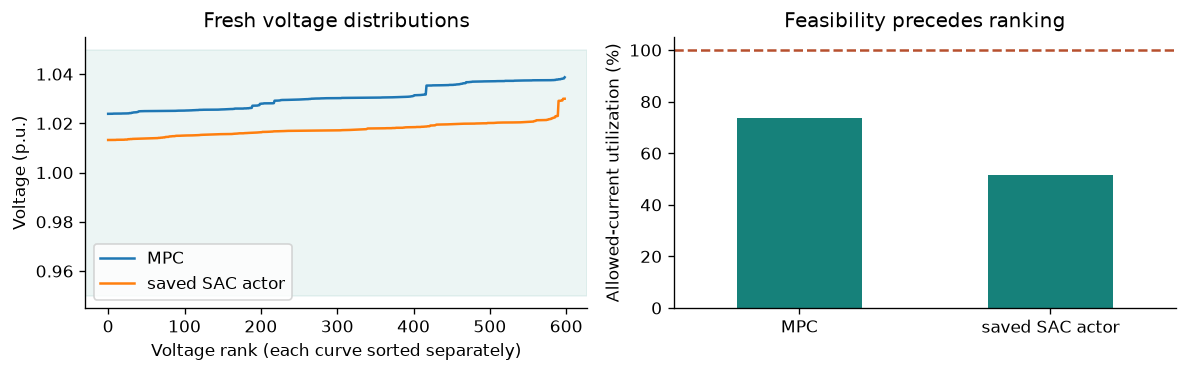
\includegraphics[width=\linewidth,height=3.65cm,keepaspectratio]{images/hands_on_L2_plot.png}
\par{\fontsize{7}{8.3}\selectfont\color{Slate} Reference L2 plots. Rerun for your chosen inputs.}
\par\endgroup\smallskip
{
\small\begin{itemize}
\setlength{\itemsep}{.25em}
\item Left: voltages should stay in the allowed band.
\item Right: current should stay below 100\% of the allowance.
\end{itemize}\par}
\vfill
{\fontsize{6.3}{7.5}\selectfont\color{Slate} Source: \href{https://colab.research.google.com/github/AlaaSelim-sudo/GridGuard-Agentic-AI-Tutorials/blob/main/agentic_grid_workflow_tutorial/Classroom_Labs.ipynb}{Classroom\_Labs.ipynb, L2; cell classroom-007; src/continuous\_control.py.}\par}
\note{**Say**

Left: voltages should stay in the allowed band. Right: current should stay below 100\% of the allowance. A value below the current line does not replace the voltage check. The same candidate must satisfy every required check.

**Show**

Use the actual source image. Point to the returned status or number that supports the slide's statement. State whether it is a fresh calculation or a saved example.

**Colab: NO NEW RUN**

Read the output from the previous run. Compare it with the reference figure; no new cell is needed.

Classroom Labs notebook. Classroom\_Labs.ipynb, L2; cell classroom-007; src/continuous\_control.py. Public notebook and Python source. 24 October 2026; stable notebook cell IDs checked.
Full source: https://github.c\allowbreak{}om/AlaaSelim-sud\allowbreak{}o/GridGuard-Agen\allowbreak{}tic-AI-Tutorials\allowbreak{}/blob/main/agent\allowbreak{}ic\_grid\_workflow\allowbreak{}\_tutorial/Classr\allowbreak{}oom\_Labs.ipynb}
\end{frame}

\begin{frame}[t]{Both pass; MPC has the lower score}
\relax
\begingroup\centering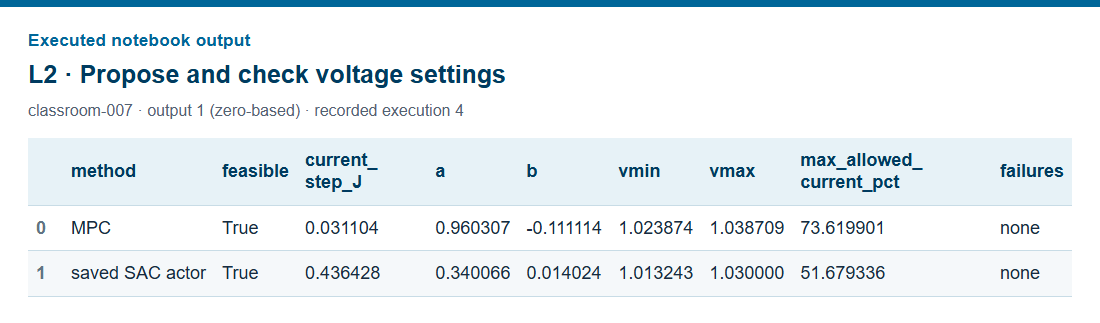
\includegraphics[width=\linewidth,height=3.65cm,keepaspectratio]{images/hands_on_L2_table.png}
\par{\fontsize{7}{8.3}\selectfont\color{Slate} Reference L2 output at load scale 1.0 and current allowance 0.80.}
\par\endgroup\smallskip
{
\small\begin{itemize}
\setlength{\itemsep}{.25em}
\item MPC: 73.62\% current use; score J about 0.03110.
\item Saved SAC: 51.68\% current use; score J about 0.43643.
\end{itemize}\par}
\vfill
{\fontsize{6.3}{7.5}\selectfont\color{Slate} Source: \href{https://colab.research.google.com/github/AlaaSelim-sudo/GridGuard-Agentic-AI-Tutorials/blob/main/agentic_grid_workflow_tutorial/Classroom_Labs.ipynb}{Classroom\_Labs.ipynb, L2; cell classroom-007; src/continuous\_control.py.}\par}
\note{**Say**

MPC: 73.62\% current use; score J about 0.03110. Saved SAC: 51.68\% current use; score J about 0.43643. SAC uses less current, but MPC has the lower cost score. This is why we must name the goal instead of selecting the smallest number in any column.

**Show**

Use the actual source image. Point to the returned status or number that supports the slide's statement. State whether it is a fresh calculation or a saved example.

**Colab: NO NEW RUN**

Read the output from the previous run. Compare it with the reference figure; no new cell is needed.

Classroom Labs notebook. Classroom\_Labs.ipynb, L2; cell classroom-007; src/continuous\_control.py. Public notebook and Python source. 24 October 2026; stable notebook cell IDs checked.
Full source: https://github.c\allowbreak{}om/AlaaSelim-sud\allowbreak{}o/GridGuard-Agen\allowbreak{}tic-AI-Tutorials\allowbreak{}/blob/main/agent\allowbreak{}ic\_grid\_workflow\allowbreak{}\_tutorial/Classr\allowbreak{}oom\_Labs.ipynb}
\end{frame}

\begin{frame}[t]{Exercise 1: lower the current allowance}
\relax
\begingroup\fontsize{10}{13}\selectfont\ttfamily\raggedright
\noindent\strut\mbox{RATING\_FRACTION~=~0.75}\par
\endgroup\medskip
{
\normalsize\begin{itemize}
\item In L2, change RATING\_FRACTION from 0.80 to 0.75. Predict, then rerun.
\item Compare pass/fail, current use and score J for both methods.
\item Does this check cover the whole medium- and low-voltage network?
\end{itemize}\par}
\vfill
{\fontsize{6.3}{7.5}\selectfont\color{Slate} Source: \href{https://colab.research.google.com/github/AlaaSelim-sudo/GridGuard-Agentic-AI-Tutorials/blob/main/agentic_grid_workflow_tutorial/Classroom_Labs.ipynb}{Classroom\_Labs.ipynb, L2; cell classroom-007; src/continuous\_control.py.}\par}
\note{**Say**

In L2, change RATING\_FRACTION from 0.80 to 0.75. Predict, then rerun. Compare pass/fail, current use and score J for both methods. Does this check cover the whole medium- and low-voltage network?

**Show**

Show the question for three minutes: predict for one, then edit and run for two. Advance once for the worked answer.

**Colab: EDIT AND RERUN**

Change only RATING\_FRACTION to 0.75. Predict, then rerun all of L2. Give this exercise four minutes.

Exact cells: classroom-007. Run the whole cell, not only the slide excerpt.

**Expected result**

MPC current use is about 78.53\%; SAC about 54.85\%; both pass this MV test.

**Ask**

In L2, change RATING\_FRACTION from 0.80 to 0.75. Predict, then rerun. Compare pass/fail, current use and score J for both methods. Does this check cover the whole medium- and low-voltage network?

**Answer**

MPC has the lower score; SAC uses less current. The score considers more than current alone. This check covers the medium-voltage model. The wider network needs a wider study. At the exercise settings, MPC uses 78.53\% of the allowance and SAC uses 54.85\%. Both pass. Their current-step scores are about 0.03110 and 0.43246.

Classroom Labs notebook. Classroom\_Labs.ipynb, L2; cell classroom-007; src/continuous\_control.py. Public notebook and Python source. 24 October 2026; stable notebook cell IDs checked.
Full source: https://github.c\allowbreak{}om/AlaaSelim-sud\allowbreak{}o/GridGuard-Agen\allowbreak{}tic-AI-Tutorials\allowbreak{}/blob/main/agent\allowbreak{}ic\_grid\_workflow\allowbreak{}\_tutorial/Classr\allowbreak{}oom\_Labs.ipynb}
\end{frame}

\begin{frame}[t]{Exercise 1 answer: both options still pass}
\relax
\begingroup\begin{minipage}[c][3.3cm][c]{\linewidth}\centering\setbox0=\hbox{\resizebox{.96\linewidth}{!}{\definecolor{Red}{HTML}{B83136}
\begin{tikzpicture}[font=\rmfamily\fontsize{12}{14}\selectfont,x=.085cm,y=1cm]
\node[anchor=west,font=\rmfamily\bfseries\fontsize{13}{15}\selectfont] at (-34,3.0) {Current used / allowance (\%)};
\node[anchor=west,text=Slate] at (-34,2.52) {L2: load scale 1.0, rating fraction 0.75};
\draw[->,Slate] (0,0)--(106,0);
\foreach \x in {0,25,50,75,100}{\draw[Slate] (\x,0)--(\x,-.08) node[below] {\x};}
\draw[Red,dashed,thick] (100,.18)--(100,2.12) node[above,text=Red] {limit};
\fill[IEEEBlue] (0,1.5) rectangle (78.527895,1.93);
\fill[Cyan] (0,.5) rectangle (54.854158,.93);
\node[anchor=east,align=right] at (-3,1.72) {MPC};
\node[anchor=east,align=right] at (-3,.72) {Saved SAC};
\node[anchor=west,font=\rmfamily\bfseries\fontsize{12}{14}\selectfont] at (79.9,1.72) {78.53};
\node[anchor=west,font=\rmfamily\bfseries\fontsize{12}{14}\selectfont] at (56.2,.72) {54.85};
\node[anchor=west,text=Slate] at (0,1.23) {$J=0.03110$ / feasible = True};
\node[anchor=west,text=Slate] at (0,.23) {$J=0.43246$ / feasible = True};
\end{tikzpicture}
}}\ifdim\dimexpr\ht0+\dp0\relax>3.3cm\resizebox{!}{3.3cm}{\box0}\else\box0\fi\par\end{minipage}\par
{\fontsize{7}{8.3}\selectfont\color{Slate} Fresh L2 exercise results. Current is shown relative to the changed allowance.\par}
\endgroup\smallskip
{
\small\begin{itemize}
\setlength{\itemsep}{.25em}
\item MPC has the lower score; SAC uses less current. The score considers more than current alone.
\item This check covers the medium-voltage model. The wider network needs a wider study.
\end{itemize}\par}
\vfill
{\fontsize{6.3}{7.5}\selectfont\color{Slate} Source: \href{https://colab.research.google.com/github/AlaaSelim-sudo/GridGuard-Agentic-AI-Tutorials/blob/main/agentic_grid_workflow_tutorial/Classroom_Labs.ipynb}{Classroom\_Labs.ipynb, L2; cell classroom-007; fresh numerical check at rating fraction 0.75.}\par}
\note{**Say**

MPC has the lower score; SAC uses less current. The score considers more than current alone. This check covers the medium-voltage model. The wider network needs a wider study. At the exercise settings, MPC uses 78.53\% of the allowance and SAC uses 54.85\%. Both pass. Their current-step scores are about 0.03110 and 0.43246.

**Show**

Advance from the exercise only after learners try it. Read the verified values, explain why the outcome occurs and answer every part of the question.

**Colab: INSPECT / RESET**

Use the output already produced for the exercise. Restore RATING\_FRACTION=0.80 and rerun all of L2 before continuing.

**Expected result**

MPC has the lower score J. The saved SAC actor uses less current; current use alone is not the objective. Both checks cover the default MV model. They do not establish full MV/LV or dynamic performance.

Classroom Labs notebook. Classroom\_Labs.ipynb, L2; cell classroom-007; src/continuous\_control.py. Public notebook and Python source. 24 October 2026; stable notebook cell IDs checked.
Full source: https://github.c\allowbreak{}om/AlaaSelim-sud\allowbreak{}o/GridGuard-Agen\allowbreak{}tic-AI-Tutorials\allowbreak{}/blob/main/agent\allowbreak{}ic\_grid\_workflow\allowbreak{}\_tutorial/Classr\allowbreak{}oom\_Labs.ipynb}
\end{frame}

\begin{frame}[t]{Less current does not mean the best option}
\relax
\begingroup\begin{minipage}[c][3.3cm][c]{\linewidth}\centering\setbox0=\hbox{\resizebox{.96\linewidth}{!}{\definecolor{Red}{HTML}{B83136}
\begin{tikzpicture}[x=1cm,y=1cm,font=\rmfamily\fontsize{12}{14}\selectfont,
 every node/.style={text=Navy,align=center},>=Latex,
 flow/.style={->,draw=IEEEBlue,line width=1.25pt},
 plainpoint/.style={circle,draw=IEEEBlue,fill=white,line width=1.25pt,minimum size=.55cm,inner sep=1pt}]

\node[anchor=west,font=\rmfamily\bfseries] at (.2,3.2) {Active-power setting: share of inverter rating};
\draw[->,Slate] (3,0)--(14,0);
\foreach \x/\v in {3/0,5.5/25,8/50,10.5/75,13/100}{\draw[Slate] (\x,0)--(\x,-.08) node[below] {\v\%};}
\node[anchor=east] at (2.7,2.05) {MPC};\node[anchor=east] at (2.7,1.05) {Saved SAC};
\fill[IEEEBlue] (3,1.8) rectangle (12.603066,2.3);
\fill[Cyan] (3,.8) rectangle (6.431254,1.3);
\node[anchor=west,font=\rmfamily\bfseries] at (12.75,2.05) {96\%};
\node[anchor=west,font=\rmfamily\bfseries] at (6.6,1.05) {34\%};

\end{tikzpicture}
}}\ifdim\dimexpr\ht0+\dp0\relax>3.3cm\resizebox{!}{3.3cm}{\box0}\else\box0\fi\par\end{minipage}\par
{\fontsize{7}{8.3}\selectfont\color{Slate} Exercise values at RATING\_FRACTION=0.75; a uses inverter rating as its base.\par}
\endgroup\smallskip
{
\small\begin{itemize}
\setlength{\itemsep}{.25em}
\item Here SAC also uses less solar output.
\item The goal values generation as well as limits. Compare the score after checks pass.
\end{itemize}\par}
\vfill
{\fontsize{6.3}{7.5}\selectfont\color{Slate} Source: \href{https://colab.research.google.com/github/AlaaSelim-sudo/GridGuard-Agentic-AI-Tutorials/blob/main/agentic_grid_workflow_tutorial/Classroom_Labs.ipynb}{Classroom Labs L2, cell classroom-007; verified default and exercise outputs.}\par}
\note{**Say**

Here SAC also uses less solar output. The goal values generation as well as limits. Compare the score after checks pass. The active-power setting is about 0.9603 for MPC and 0.3431 for SAC in this exercise. Lower solar output can reduce current but also increase the stated cost.

**Show**

Read the visual from the input to the result. Name the operator's goal, the agent's request and the fact supplied by the tool. Explain the decision in the two slide sentences.

**Colab: NO NEW RUN**

Read the output from the previous run. Compare it with the reference figure; no new cell is needed.

Classroom Labs notebook. Classroom\_Labs.ipynb, L2; cell classroom-007; src/continuous\_control.py. Public notebook and Python source. 24 October 2026; stable notebook cell IDs checked.
Full source: https://github.c\allowbreak{}om/AlaaSelim-sud\allowbreak{}o/GridGuard-Agen\allowbreak{}tic-AI-Tutorials\allowbreak{}/blob/main/agent\allowbreak{}ic\_grid\_workflow\allowbreak{}\_tutorial/Classr\allowbreak{}oom\_Labs.ipynb}
\end{frame}

\begin{frame}[t]{Back to the starting values}
\relax
{\fontsize{8}{10}\selectfont\color{Slate} Run the whole cell in Colab\par}\smallskip
\lstinputlisting[basicstyle=\ttfamily\fontsize{12}{14.5}\selectfont,aboveskip=3pt,belowskip=10pt,breaklines=true,gobble=0]{../research/code/voltage_Classroom_Labs_classroom-007_L1-2.py}
{
\small\begin{itemize}
\setlength{\itemsep}{.25em}
\item Restore LOAD\_SCALE=1.0 and RATING\_FRACTION=0.80. Rerun L2.
\item The next cells use a separate saved case.
\end{itemize}\par}
\vfill
{\fontsize{6.3}{7.5}\selectfont\color{Slate} Source: \href{https://colab.research.google.com/github/AlaaSelim-sudo/GridGuard-Agentic-AI-Tutorials/blob/main/agentic_grid_workflow_tutorial/Classroom_Labs.ipynb}{Classroom\_Labs.ipynb, L2; cell classroom-007; src/continuous\_control.py.}\par}
\note{**Say**

Restore LOAD\_SCALE=1.0 and RATING\_FRACTION=0.80. Rerun L2. The next cells use a separate saved case. Resetting keeps the class together. The following saved case has its own original inputs; your changed L2 settings do not rewrite it.

**Show**

Locate L2 in Classroom Labs. Show the highlighted source lines, then run the whole cell when the Colab cue says to run. Read the returned result in plain words.

**Colab: RESET AND RERUN**

Restore LOAD\_SCALE=1.0 and RATING\_FRACTION=0.80; rerun the complete L2 cell.

Exact cells: classroom-007. Run the whole cell, not only the slide excerpt.

**Expected result**

The default output returns. L3-L5 will use their separate original test\_01 case.

Classroom Labs notebook. Classroom\_Labs.ipynb, L2; cell classroom-007; src/continuous\_control.py. Public notebook and Python source. 24 October 2026; stable notebook cell IDs checked.
Full source: https://github.c\allowbreak{}om/AlaaSelim-sud\allowbreak{}o/GridGuard-Agen\allowbreak{}tic-AI-Tutorials\allowbreak{}/blob/main/agent\allowbreak{}ic\_grid\_workflow\allowbreak{}\_tutorial/Classr\allowbreak{}oom\_Labs.ipynb}
\end{frame}

\begin{frame}[t]{Separate a new calculation from a replay}
\relax
\begingroup\begin{minipage}[c][3.3cm][c]{\linewidth}\centering\setbox0=\hbox{\resizebox{.96\linewidth}{!}{\definecolor{Red}{HTML}{B83136}
\begin{tikzpicture}[x=1cm,y=1cm,font=\rmfamily\fontsize{12}{14}\selectfont,
 every node/.style={text=Navy,align=center},>=Latex,
 flow/.style={->,draw=IEEEBlue,line width=1.25pt},
 plainpoint/.style={circle,draw=IEEEBlue,fill=white,line width=1.25pt,minimum size=.55cm,inner sep=1pt}]

\node[anchor=west,font=\rmfamily\bfseries] at (0,3.1) {A fresh calculation};
\node at (1.5,2.25) {Your inputs};\node at (7,2.25) {Python runs now};\node at (12.5,2.25) {New numbers};
\draw[flow] (3.1,2.25)--(5.3,2.25);\draw[flow] (8.8,2.25)--(11,2.25);
\node[anchor=west,font=\rmfamily\bfseries] at (0,.85) {A recorded replay};
\node at (1.5,0) {Original inputs};\node[text width=4cm] at (7,0) {Saved Llama choice};\node[text width=3cm] at (12.5,0) {Past result};
\draw[flow] (3.1,0)--(5.2,0);\draw[flow] (8.8,0)--(11,0);

\end{tikzpicture}
}}\ifdim\dimexpr\ht0+\dp0\relax>3.3cm\resizebox{!}{3.3cm}{\box0}\else\box0\fi\par\end{minipage}\par
{\fontsize{7}{8.3}\selectfont\color{Slate} A replay keeps its original inputs, decisions and results.\par}
\endgroup\smallskip
{
\small\begin{itemize}
\setlength{\itemsep}{.25em}
\item Your inputs produce new numerical results.
\item Saved replies show past model decisions; editing L2 does not change them.
\end{itemize}\par}
\vfill
{\fontsize{6.3}{7.5}\selectfont\color{Slate} Source: \href{https://github.com/AlaaSelim-sudo/GridGuard-Agentic-AI-Tutorials/blob/main/COLAB_GUIDE.md}{Classroom Labs notebook. Setup: COLAB\_GUIDE.md; Classroom\_Labs.ipynb. Public notebook and Python source. 24 October 2026; stable notebook cell IDs checked.}\par}
\note{**Say**

Your inputs produce new numerical results. Saved replies show past model decisions; editing L2 does not change them. A fresh calculation answers the inputs you just supplied. A replay shows what happened previously. Both are useful, but they answer different questions.

**Show**

Read the visual from the input to the result. Name the operator's goal, the agent's request and the fact supplied by the tool. Explain the decision in the two slide sentences.

**Colab: NO NEW RUN**

Explain the figure or discuss the output already produced. Do not run ahead.

Classroom Labs notebook. Setup: COLAB\_GUIDE.md; Classroom\_Labs.ipynb. Public notebook and Python source. 24 October 2026; stable notebook cell IDs checked.
Full source: https://github.c\allowbreak{}om/AlaaSelim-sud\allowbreak{}o/GridGuard-Agen\allowbreak{}tic-AI-Tutorials\allowbreak{}/blob/main/COLAB\allowbreak{}\_GUIDE.md

Classroom Labs notebook and Python helper. L10B: Watch how Llama chooses a tool; src/llama\_walkthrough.py. Public reproducible teaching material. 24 October 2026.
Full source: https://github.c\allowbreak{}om/AlaaSelim-sud\allowbreak{}o/GridGuard-Agen\allowbreak{}tic-AI-Tutorials\allowbreak{}/blob/main/agent\allowbreak{}ic\_grid\_workflow\allowbreak{}\_tutorial/src/ll\allowbreak{}ama\_walkthrough.\allowbreak{}py

Keith Stouffer, Michael Pease, CheeYee Tang, Timothy Zimmerman, Victoria Pillitteri, Suzanne Lightman, Adam Hahn, Stephanie Saravia, Aslam Sherule, Michael Thompson. Guide to Operational Technology (OT) Security. National Institute of Standards and Technology, NIST SP 800-82 Revision 3. September 2023 (final).
Full source: https://doi.org/10.6028/NIST.SP.800-82r3
Full paper: https://nvlpubs.\allowbreak{}nist.gov/nistpub\allowbreak{}s/SpecialPublica\allowbreak{}tions/NIST.SP.80\allowbreak{}0-82r3.pdf
Publication: https://csrc.nis\allowbreak{}t.gov/pubs/sp/80\allowbreak{}0/82/r3/final}
\end{frame}

\begin{frame}[t]{What did the saved models choose?}
\relax
{\fontsize{8}{10}\selectfont\color{Slate} Run the whole cell in Colab\par}\smallskip
\lstinputlisting[basicstyle=\ttfamily\fontsize{12}{14.5}\selectfont,aboveskip=3pt,belowskip=10pt,breaklines=true,gobble=0]{../research/code/voltage_Classroom_Labs_classroom-010_L1-1.py}
{
\small\begin{itemize}
\setlength{\itemsep}{.25em}
\item Run L3 to see what the models requested for the saved case.
\item This displays old replies; it makes no new model call.
\end{itemize}\par}
\vfill
{\fontsize{6.3}{7.5}\selectfont\color{Slate} Source: \href{https://colab.research.google.com/github/AlaaSelim-sudo/GridGuard-Agentic-AI-Tutorials/blob/main/agentic_grid_workflow_tutorial/Classroom_Labs.ipynb}{Classroom\_Labs.ipynb, L3; cell classroom-010; archived test\_01 context.}\par}
\note{**Say**

Run L3 to see what the models requested for the saved case. This displays old replies; it makes no new model call. Read the request, reason and recorded time as a historical record. The model is not responding to your new L2 input.

**Show**

Locate L3 in Classroom Labs. Show the highlighted source lines, then run the whole cell when the Colab cue says to run. Read the returned result in plain words.

**Colab: RUN**

Run L3. Keep the default test\_01 case.

Exact cells: classroom-010. Run the whole cell, not only the slide excerpt.

**Expected result**

Three saved model replies and recorded times appear; no new model request occurs.

Classroom Labs notebook. Classroom\_Labs.ipynb, L3; cell classroom-010; archived test\_01 context. Public notebook and Python source. 24 October 2026; stable notebook cell IDs checked.
Full source: https://github.c\allowbreak{}om/AlaaSelim-sud\allowbreak{}o/GridGuard-Agen\allowbreak{}tic-AI-Tutorials\allowbreak{}/blob/main/agent\allowbreak{}ic\_grid\_workflow\allowbreak{}\_tutorial/Classr\allowbreak{}oom\_Labs.ipynb}
\end{frame}

\begin{frame}[t]{Different replies can request the same action}
\relax
\begingroup\begin{minipage}[c][3.25cm][c]{\linewidth}\centering\setbox0=\hbox{\resizebox{.96\linewidth}{!}{\definecolor{IEEEBlue}{HTML}{00629B}
\definecolor{Cyan}{HTML}{00A6B2}
\definecolor{Navy}{HTML}{003B5C}
\definecolor{Slate}{HTML}{526470}
\definecolor{AlertRed}{HTML}{B83136}
\definecolor{Amber}{HTML}{A66610}
\begin{tikzpicture}[x=1cm,y=1cm,>=Latex,
 font=\fontsize{11}{13}\selectfont,text=Navy,
 box/.style={draw=IEEEBlue,thick,rounded corners=2pt,align=center,
 fill=IEEEBlue!4,inner sep=3pt,minimum height=.62cm},
 arr/.style={->,draw=IEEEBlue,line width=1pt},
 ]

\node[box,text width=2.15cm] (l1) at (1.25,1.00) {Llama 3.1};
\node[box,text width=2.15cm] (l2) at (1.25,0) {Llama 3.2};
\node[box,text width=2.15cm] (qw) at (1.25,-1.00) {Qwen 2.5};
\node[box,text width=3.05cm] (active) at (5.55,.80) {$(a+0.0025,b)$\\one vote};
\node[box,text width=3.05cm,draw=Cyan,fill=Cyan!8] (reactive) at (5.55,-.80) {$(a,0.9b)$\\two votes};
\node[box,text width=3.25cm] (trial) at (10.75,-.80) {Numerical trial\\$a=0.960307$\\$b=-0.100002$};
\node[align=center] at (10.75,.80) {Three replies\\two physical actions};
\draw[arr] (l1.east)--(active.west);
\draw[arr] (l2.east)--(reactive.west);
\draw[arr] (qw.east)--(reactive.west);
\draw[arr,draw=Cyan] (reactive.east)--(trial.west);

\end{tikzpicture}
}}\ifdim\dimexpr\ht0+\dp0\relax>3.25cm\resizebox{!}{3.25cm}{\box0}\else\box0\fi\par\end{minipage}\par
{\fontsize{7}{8.3}\selectfont\color{Slate} Three saved replies request two different trials.\par}
\endgroup\smallskip
{
\small\begin{itemize}
\setlength{\itemsep}{.25em}
\item Group requests that describe the same settings.
\item A vote chooses what to test next. The electrical check still has to run.
\end{itemize}\par}
\vfill
{\fontsize{6.3}{7.5}\selectfont\color{Slate} Source: \href{https://colab.research.google.com/github/AlaaSelim-sudo/GridGuard-Agentic-AI-Tutorials/blob/main/agentic_grid_workflow_tutorial/Classroom_Labs.ipynb}{Classroom\_Labs.ipynb, L3; cell classroom-010; archived test\_01 context.}\par}
\note{**Say**

Group requests that describe the same settings. A vote chooses what to test next. The electrical check still has to run. Wording alone should not create extra votes for the same physical operation. The numerical check still determines whether the selected setting passes.

**Show**

Use the two short slide statements to explain the idea. Link it to the operator's next decision or to the named Colab cell.

**Colab: NO NEW RUN**

Explain the figure or discuss the output already produced. Do not run ahead.

Classroom Labs notebook. Classroom\_Labs.ipynb, L3; cell classroom-010; archived test\_01 context. Public notebook and Python source. 24 October 2026; stable notebook cell IDs checked.
Full source: https://github.c\allowbreak{}om/AlaaSelim-sud\allowbreak{}o/GridGuard-Agen\allowbreak{}tic-AI-Tutorials\allowbreak{}/blob/main/agent\allowbreak{}ic\_grid\_workflow\allowbreak{}\_tutorial/Classr\allowbreak{}oom\_Labs.ipynb}
\end{frame}

\begin{frame}[t]{A fresh check of the chosen proposal}
\relax
{\fontsize{8}{10}\selectfont\color{Slate} Run the whole cell in Colab\par}\smallskip
\lstinputlisting[basicstyle=\ttfamily\fontsize{12}{14.5}\selectfont,aboveskip=3pt,belowskip=10pt,breaklines=true,gobble=0]{../research/code/voltage_Classroom_Labs_classroom-013_L6-6.py}
{
\small\begin{itemize}
\setlength{\itemsep}{.25em}
\item Run L4 to check the chosen proposal again in its original case.
\item Both selectors choose the same action here, and the fresh electrical checks pass.
\end{itemize}\par}
\vfill
{\fontsize{6.3}{7.5}\selectfont\color{Slate} Source: \href{https://colab.research.google.com/github/AlaaSelim-sudo/GridGuard-Agentic-AI-Tutorials/blob/main/agentic_grid_workflow_tutorial/Classroom_Labs.ipynb}{Classroom\_Labs.ipynb, L4; cell classroom-013; fresh checks of archived choices.}\par}
\note{**Say**

Run L4 to check the chosen proposal again in its original case. Both selectors choose the same action here, and the fresh electrical checks pass. The selection score and the engineering check do different jobs. A selected action must still be checked.

**Show**

Locate L4 in Classroom Labs. Show the highlighted source lines, then run the whole cell when the Colab cue says to run. Read the returned result in plain words.

**Colab: RUN**

Run L4 after L3 without changing the case ID.

Exact cells: classroom-013. Run the whole cell, not only the slide excerpt.

**Expected result**

Both selectors choose RELAX\_Q\_10\_PERCENT. Both new electrical checks pass.

Classroom Labs notebook. Classroom\_Labs.ipynb, L4; cell classroom-013; fresh checks of archived choices. Public notebook and Python source. 24 October 2026; stable notebook cell IDs checked.
Full source: https://github.c\allowbreak{}om/AlaaSelim-sud\allowbreak{}o/GridGuard-Agen\allowbreak{}tic-AI-Tutorials\allowbreak{}/blob/main/agent\allowbreak{}ic\_grid\_workflow\allowbreak{}\_tutorial/Classr\allowbreak{}oom\_Labs.ipynb}
\end{frame}

\begin{frame}[t]{Which part of the grid was checked?}
\relax
{\fontsize{8}{10}\selectfont\color{Slate} Run the whole cell in Colab\par}\smallskip
\lstinputlisting[basicstyle=\ttfamily\fontsize{12}{14.5}\selectfont,aboveskip=3pt,belowskip=10pt,breaklines=true,gobble=0]{../research/code/voltage_Classroom_Labs_classroom-016_L2-2.py}
{
\small\begin{itemize}
\setlength{\itemsep}{.25em}
\item Run L5 with the default settings.
\item It checks the medium-voltage (MV) part of the saved case.
\end{itemize}\par}
\vfill
{\fontsize{6.3}{7.5}\selectfont\color{Slate} Source: \href{https://colab.research.google.com/github/AlaaSelim-sudo/GridGuard-Agentic-AI-Tutorials/blob/main/agentic_grid_workflow_tutorial/Classroom_Labs.ipynb}{Classroom\_Labs.ipynb, L5; cell classroom-016; MV-only default model.}\par}
\note{**Say**

Run L5 with the default settings. It checks the medium-voltage (MV) part of the saved case. The wider OpenDSS study is disabled by default. This cell therefore supports a medium-voltage claim only.

**Show**

Locate L5 in Classroom Labs. Show the highlighted source lines, then run the whole cell when the Colab cue says to run. Read the returned result in plain words.

**Colab: RUN**

Run L5 with RUN\_OPENDSS still False.

Exact cells: classroom-016. Run the whole cell, not only the slide excerpt.

**Expected result**

The linear-model check is shown; the optional full-model path is disabled.

Classroom Labs notebook. Classroom\_Labs.ipynb, L5; cell classroom-016; MV-only default model. Public notebook and Python source. 24 October 2026; stable notebook cell IDs checked.
Full source: https://github.c\allowbreak{}om/AlaaSelim-sud\allowbreak{}o/GridGuard-Agen\allowbreak{}tic-AI-Tutorials\allowbreak{}/blob/main/agent\allowbreak{}ic\_grid\_workflow\allowbreak{}\_tutorial/Classr\allowbreak{}oom\_Labs.ipynb}
\end{frame}

\begin{frame}[t]{A PASS covers only what was checked}
\relax
\begingroup\centering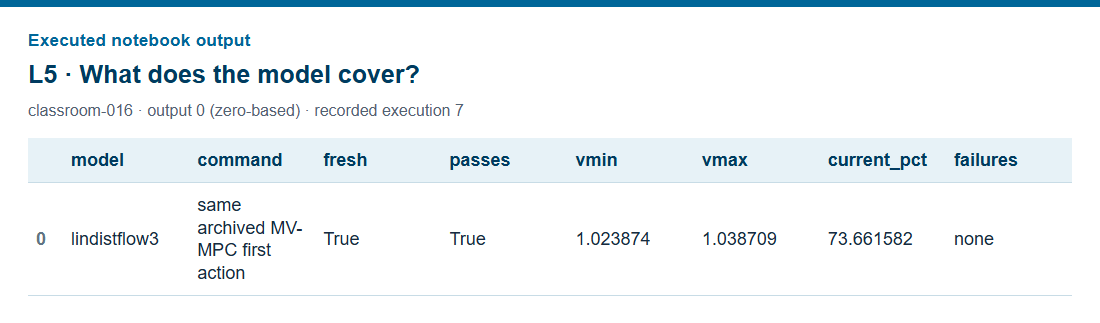
\includegraphics[width=\linewidth,height=2.95cm,keepaspectratio]{images/hands_on_L5_scope.png}
\par{\fontsize{7}{8.3}\selectfont\color{Slate} Reference L5 result covers medium voltage only.}
\par\endgroup\smallskip
{
\small\begin{itemize}
\setlength{\itemsep}{.25em}
\item A limited model cannot answer a wider grid question.
\item Request the missing study or return HOLD.
\end{itemize}\par}
\vfill
{\fontsize{6.3}{7.5}\selectfont\color{Slate} Source: \href{https://colab.research.google.com/github/AlaaSelim-sudo/GridGuard-Agentic-AI-Tutorials/blob/main/agentic_grid_workflow_tutorial/Classroom_Labs.ipynb}{Classroom\_Labs.ipynb, L5; cell classroom-016; MV-only default model.}\par}
\note{**Say**

A limited model cannot answer a wider grid question. Request the missing study or return HOLD. A checked part of a network does not stand for every device or every operating limit. Ask for the check needed by the actual decision.

**Show**

Use the actual source image. Point to the returned status or number that supports the slide's statement. State whether it is a fresh calculation or a saved example.

**Colab: NO NEW RUN**

Read the output from the previous run. Compare it with the reference figure; no new cell is needed.

Classroom Labs notebook. Classroom\_Labs.ipynb, L5; cell classroom-016; MV-only default model. Public notebook and Python source. 24 October 2026; stable notebook cell IDs checked.
Full source: https://github.c\allowbreak{}om/AlaaSelim-sud\allowbreak{}o/GridGuard-Agen\allowbreak{}tic-AI-Tutorials\allowbreak{}/blob/main/agent\allowbreak{}ic\_grid\_workflow\allowbreak{}\_tutorial/Classr\allowbreak{}oom\_Labs.ipynb}
\end{frame}

\begin{frame}[t]{Recorded example: the first option fails}
\relax
\begingroup\centering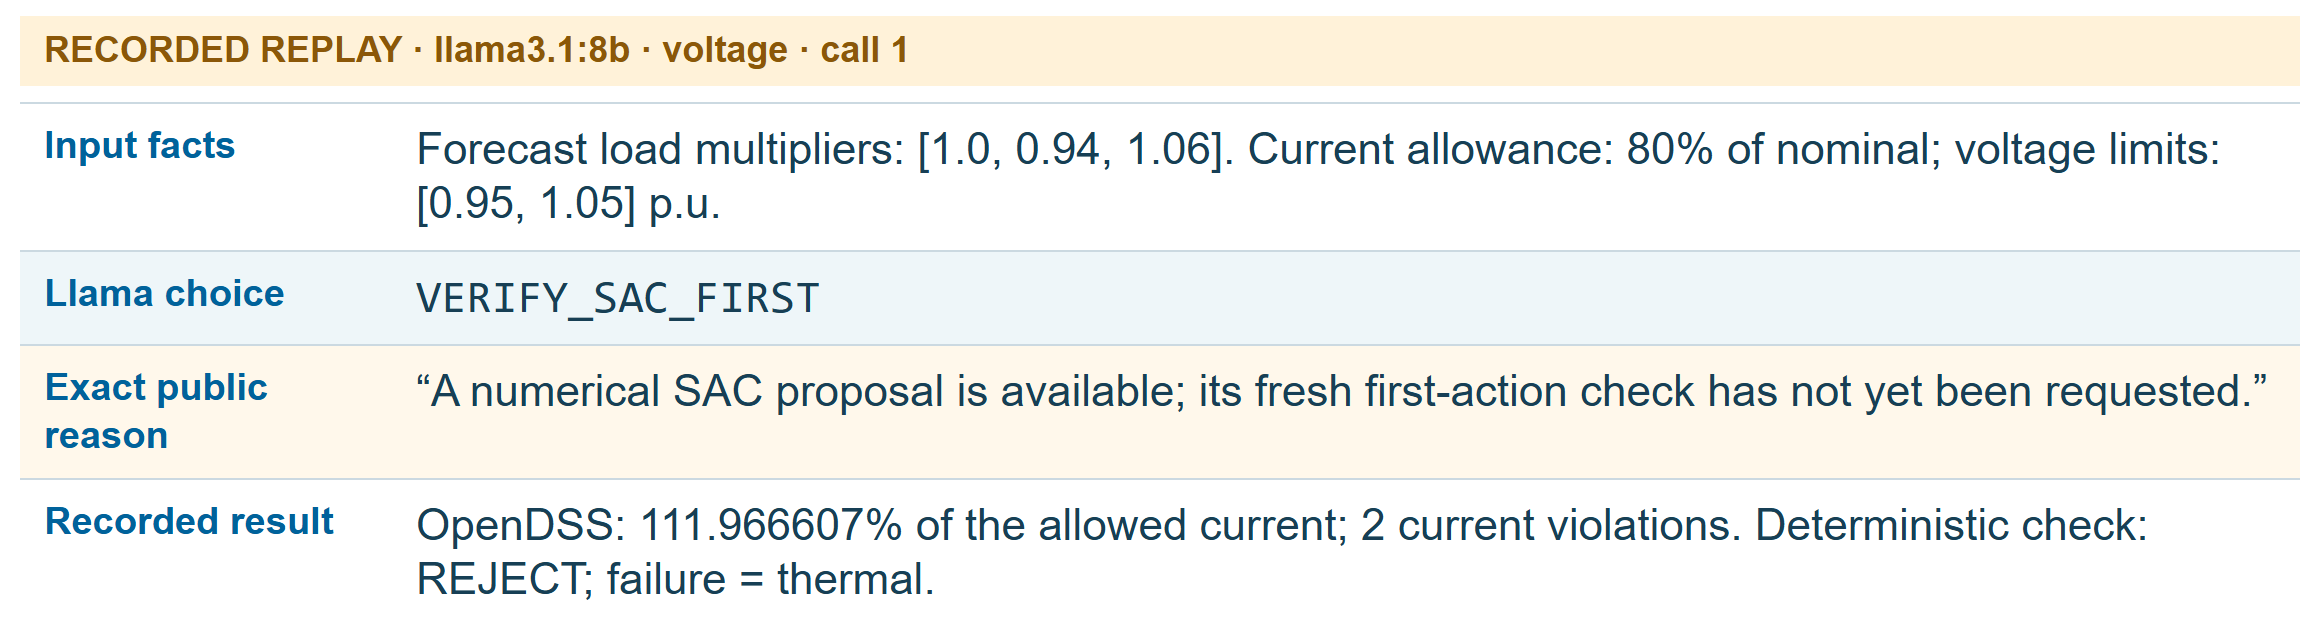
\includegraphics[width=\linewidth,height=4cm,keepaspectratio]{images/llama_voltage_1.png}
\par\endgroup\smallskip
{
\small\begin{itemize}
\setlength{\itemsep}{.25em}
\item This saved study is different from your L2 run.
\item Llama asks for a SAC check. The tool reports too much current.
\end{itemize}\par}
\vfill
{\fontsize{6.3}{7.5}\selectfont\color{Slate} Source: \href{https://colab.research.google.com/github/AlaaSelim-sudo/GridGuard-Agentic-AI-Tutorials/blob/main/agentic_grid_workflow_tutorial/Classroom_Labs.ipynb}{Classroom Labs L10B: voltage replay, recorded call 1; full record in source guide.}\par}
\note{**Say**

This saved study is different from your L2 run. Llama asks for a SAC check. The tool reports too much current. This is a preview of a different saved study, not a continuation of the passing L2 results. The recorded tool result reports a current-limit failure. The next agent choice follows that evidence.

**Show**

Preview the actual saved Llama request and returned tool evidence. Do not ask learners to run ahead. L10B will replay these records after the three labs.

**Colab: PREVIEW ONLY**

Show the slide only. Run L10B later on slide 64; keep the notebook in order.

**Expected result**

No new notebook output on this slide.

Workshop recorded model replies and numerical study records. Voltage P3\_current\_reserve: Llama 3.1:8b planner, recovery and review calls 1--3. Public teaching archive. 27 September 2026.
Full source: https://github.c\allowbreak{}om/AlaaSelim-sud\allowbreak{}o/GridGuard-Agen\allowbreak{}tic-AI-Tutorials\allowbreak{}/blob/main/agent\allowbreak{}ic\_grid\_workflow\allowbreak{}\_tutorial/result\allowbreak{}s/continuous\_lla\allowbreak{}ma\_opendss\_20260\allowbreak{}927T161223523552\allowbreak{}Z.json

Classroom Labs notebook and Python helper. L10B: Watch how Llama chooses a tool; src/llama\_walkthrough.py. Public reproducible teaching material. 24 October 2026.
Full source: https://github.c\allowbreak{}om/AlaaSelim-sud\allowbreak{}o/GridGuard-Agen\allowbreak{}tic-AI-Tutorials\allowbreak{}/blob/main/agent\allowbreak{}ic\_grid\_workflow\allowbreak{}\_tutorial/src/ll\allowbreak{}ama\_walkthrough.\allowbreak{}py}
\end{frame}

\begin{frame}[t]{Recorded example: request another option}
\relax
\begingroup\centering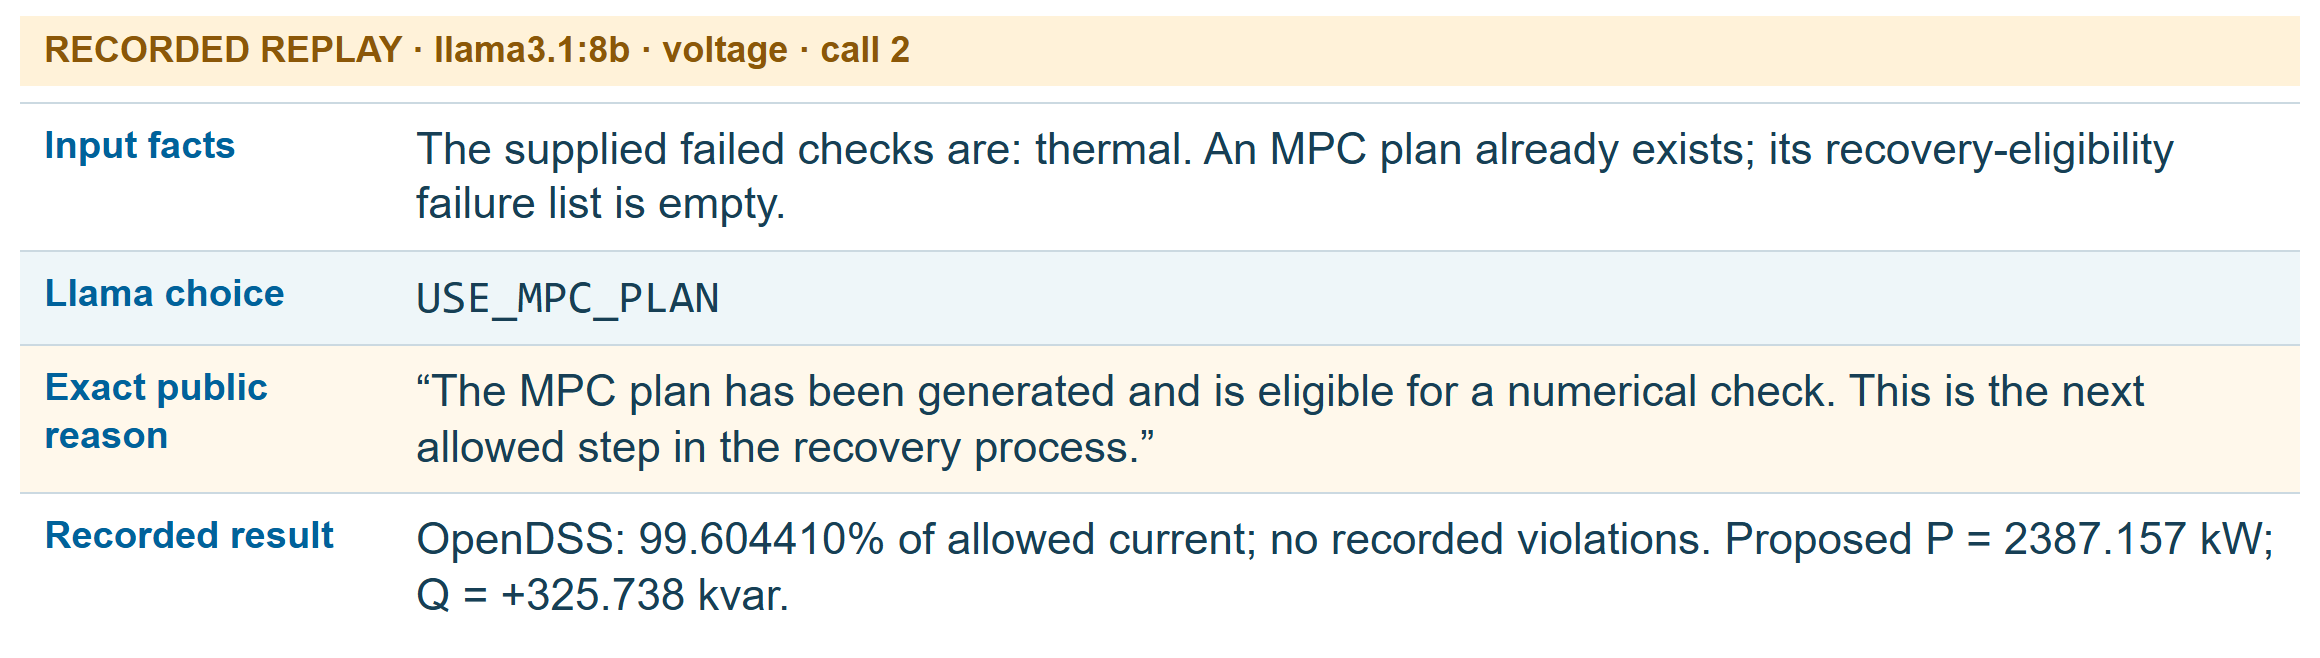
\includegraphics[width=\linewidth,height=4cm,keepaspectratio]{images/llama_voltage_2.png}
\par\endgroup\smallskip
{
\small\begin{itemize}
\setlength{\itemsep}{.25em}
\item Llama asks the tool to check the existing MPC fallback.
\item The returned electrical checks pass for this saved case.
\end{itemize}\par}
\vfill
{\fontsize{6.3}{7.5}\selectfont\color{Slate} Source: \href{https://colab.research.google.com/github/AlaaSelim-sudo/GridGuard-Agentic-AI-Tutorials/blob/main/agentic_grid_workflow_tutorial/Classroom_Labs.ipynb}{Classroom Labs L10B: voltage replay, recorded call 2; full record in source guide.}\par}
\note{**Say**

Llama asks the tool to check the existing MPC fallback. The returned electrical checks pass for this saved case. The agent requests a plan that already exists rather than inventing its electrical outcome. The tool calculates the check and returns the evidence.

**Show**

Preview the actual saved Llama request and returned tool evidence. Do not ask learners to run ahead. L10B will replay these records after the three labs.

**Colab: PREVIEW ONLY**

Show the slide only. Run L10B later on slide 64; keep the notebook in order.

**Expected result**

No new notebook output on this slide.

Workshop recorded model replies and numerical study records. Voltage P3\_current\_reserve: Llama 3.1:8b planner, recovery and review calls 1--3. Public teaching archive. 27 September 2026.
Full source: https://github.c\allowbreak{}om/AlaaSelim-sud\allowbreak{}o/GridGuard-Agen\allowbreak{}tic-AI-Tutorials\allowbreak{}/blob/main/agent\allowbreak{}ic\_grid\_workflow\allowbreak{}\_tutorial/result\allowbreak{}s/continuous\_lla\allowbreak{}ma\_opendss\_20260\allowbreak{}927T161223523552\allowbreak{}Z.json

Classroom Labs notebook and Python helper. L10B: Watch how Llama chooses a tool; src/llama\_walkthrough.py. Public reproducible teaching material. 24 October 2026.
Full source: https://github.c\allowbreak{}om/AlaaSelim-sud\allowbreak{}o/GridGuard-Agen\allowbreak{}tic-AI-Tutorials\allowbreak{}/blob/main/agent\allowbreak{}ic\_grid\_workflow\allowbreak{}\_tutorial/src/ll\allowbreak{}ama\_walkthrough.\allowbreak{}py}
\end{frame}

\begin{frame}[t]{Recorded example: return to the operator}
\relax
\begingroup\centering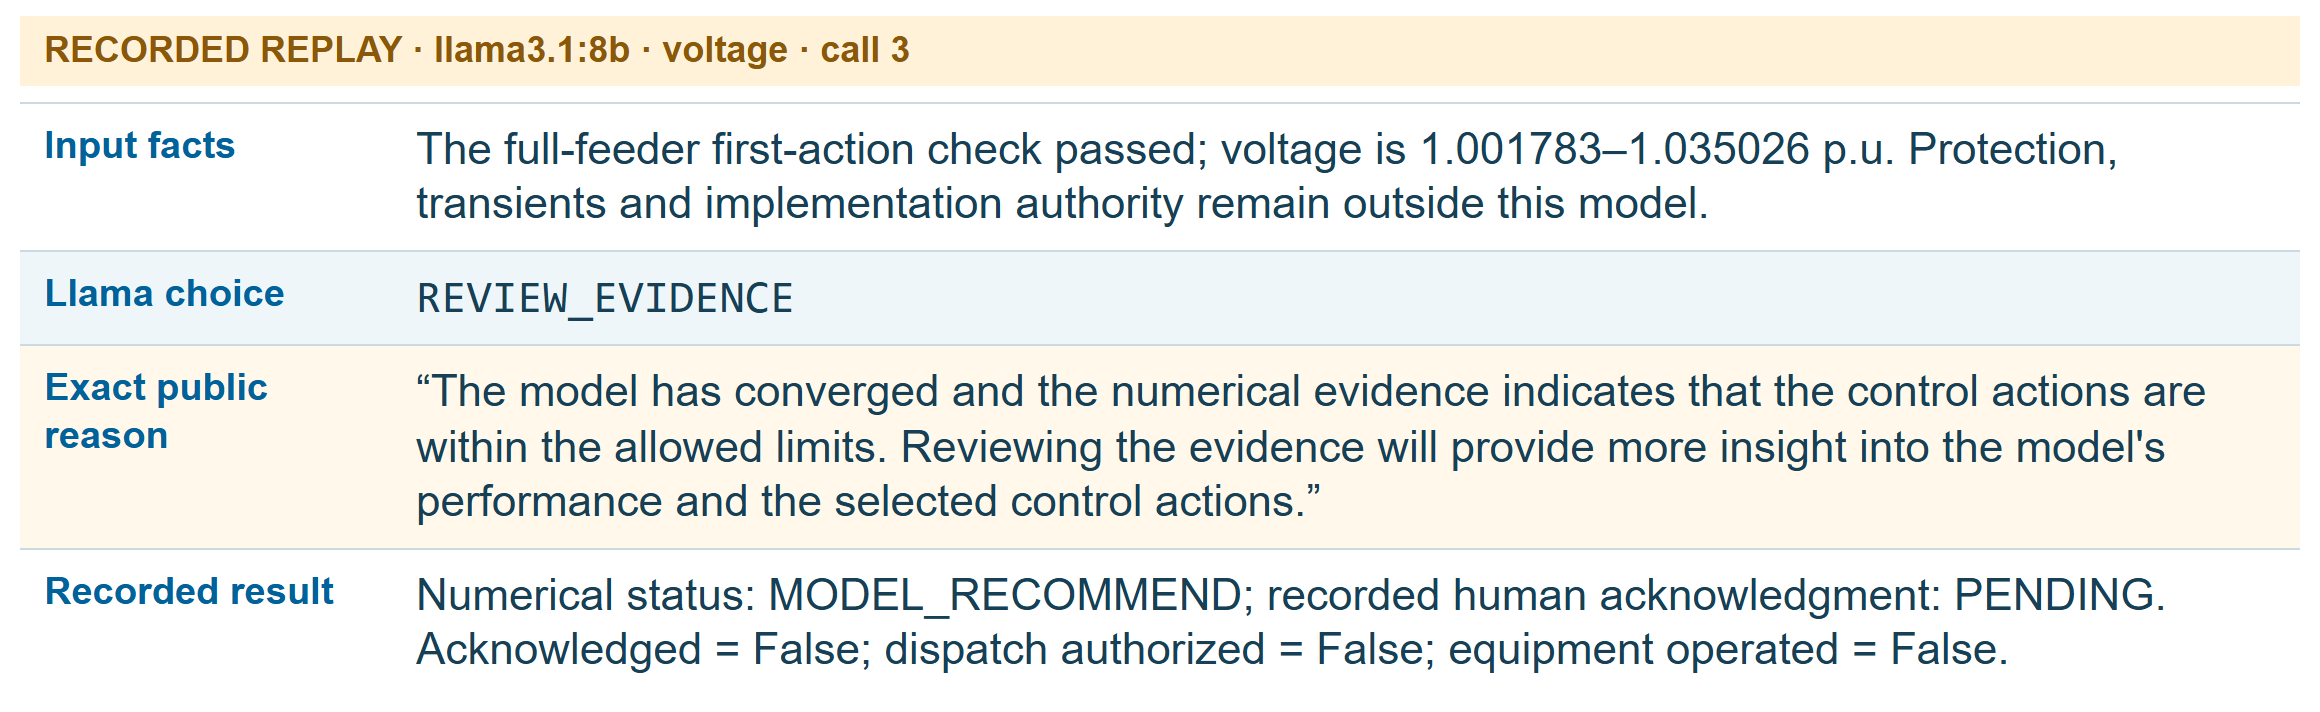
\includegraphics[width=\linewidth,height=4cm,keepaspectratio]{images/llama_voltage_3.png}
\par\endgroup\smallskip
{
\small\begin{itemize}
\setlength{\itemsep}{.25em}
\item The agent returns the checked proposal and its conditions.
\item Human review is still pending. No equipment command is sent.
\end{itemize}\par}
\vfill
{\fontsize{6.3}{7.5}\selectfont\color{Slate} Source: \href{https://colab.research.google.com/github/AlaaSelim-sudo/GridGuard-Agentic-AI-Tutorials/blob/main/agentic_grid_workflow_tutorial/Classroom_Labs.ipynb}{Classroom Labs L10B: voltage replay, recorded call 3; full record in source guide.}\par}
\note{**Say**

The agent returns the checked proposal and its conditions. Human review is still pending. No equipment command is sent. The result is a recommendation for review. The record still shows human acknowledgement pending and equipment dispatch disabled.

**Show**

Preview the actual saved Llama request and returned tool evidence. Do not ask learners to run ahead. L10B will replay these records after the three labs.

**Colab: PREVIEW ONLY**

Show the slide only. Run L10B later on slide 64; keep the notebook in order.

**Expected result**

No new notebook output on this slide.

Workshop recorded model replies and numerical study records. Voltage P3\_current\_reserve: Llama 3.1:8b planner, recovery and review calls 1--3. Public teaching archive. 27 September 2026.
Full source: https://github.c\allowbreak{}om/AlaaSelim-sud\allowbreak{}o/GridGuard-Agen\allowbreak{}tic-AI-Tutorials\allowbreak{}/blob/main/agent\allowbreak{}ic\_grid\_workflow\allowbreak{}\_tutorial/result\allowbreak{}s/continuous\_lla\allowbreak{}ma\_opendss\_20260\allowbreak{}927T161223523552\allowbreak{}Z.json

Classroom Labs notebook and Python helper. L10B: Watch how Llama chooses a tool; src/llama\_walkthrough.py. Public reproducible teaching material. 24 October 2026.
Full source: https://github.c\allowbreak{}om/AlaaSelim-sud\allowbreak{}o/GridGuard-Agen\allowbreak{}tic-AI-Tutorials\allowbreak{}/blob/main/agent\allowbreak{}ic\_grid\_workflow\allowbreak{}\_tutorial/src/ll\allowbreak{}ama\_walkthrough.\allowbreak{}py}
\end{frame}

\begin{frame}[t]{Case 2: who gets power after a fault?}
\relax
\begingroup\begin{minipage}[c][3.3cm][c]{\linewidth}\centering\setbox0=\hbox{\resizebox{.96\linewidth}{!}{\definecolor{Red}{HTML}{B83136}
\begin{tikzpicture}[x=1cm,y=1cm,font=\rmfamily\fontsize{12}{14}\selectfont,
 every node/.style={text=Navy,align=center},>=Latex,
 flow/.style={->,draw=IEEEBlue,line width=1.25pt},
 plainpoint/.style={circle,draw=IEEEBlue,fill=white,line width=1.25pt,minimum size=.55cm,inner sep=1pt}]

\node[plainpoint] (r0) at (.5,1.5) {0};\node[left=.18cm of r0] {Supply};
\node[plainpoint] (r1) at (3,2.6) {1};\node[plainpoint,draw=Cyan,line width=2pt] (r2) at (7,2.6) {2};
\node[plainpoint] (r3) at (11,1.5) {3};\node[plainpoint] (r4) at (8,.1) {4};
\node[plainpoint,draw=Cyan,line width=2pt] (r5) at (3.4,.1) {5};
\draw[IEEEBlue,thick] (r0)--(r1);\draw[IEEEBlue,thick] (r2)--(r3)--(r4);\draw[IEEEBlue,thick] (r2)--(r5);
\draw[Red,dashed,line width=1.6pt] (r1)--(r2);\node[text=Red,above] at (5,2.7) {Fault: unavailable};
\draw[Cyan,dashed,line width=1.3pt] (r0.south)--(r4.south);\draw[Cyan,dashed,line width=1.3pt] (r1)--(r5);
\node[above=.25cm of r2,text=Cyan] {Critical load};\node[below=.25cm of r5,text=Cyan] {Critical load};
\node[right=.25cm of r3] {Other load};\node[right=.25cm of r4] {Other load};


\end{tikzpicture}
}}\ifdim\dimexpr\ht0+\dp0\relax>3.3cm\resizebox{!}{3.3cm}{\box0}\else\box0\fi\par\end{minipage}\par
{\fontsize{7}{8.3}\selectfont\color{Slate} Six-node lab graph. Cyan marks critical loads; dashed links are backup options.\par}
\endgroup\smallskip
{
\small\begin{itemize}
\setlength{\itemsep}{.25em}
\item A fault removes a supply path. Available capacity limits what can be restored.
\item The operator sets priorities; the agent can request and check restoration options.
\end{itemize}\par}
\vfill
{\fontsize{6.3}{7.5}\selectfont\color{Slate} Source: \href{https://colab.research.google.com/github/AlaaSelim-sudo/GridGuard-Agentic-AI-Tutorials/blob/main/agentic_grid_workflow_tutorial/Classroom_Labs.ipynb}{Classroom\_Labs.ipynb, L6; cell classroom-018; src/standard\_formulations.py.}\par}
\note{**Say**

A fault removes one normal supply path. Alternative paths have limited capacity, so the operator must choose what to restore. Serving critical demand first can differ from maximizing the total power served. The agent can carry that priority into a study request, collect the result and request a new study when the situation changes.

**Show**

Read the visual from the input to the result. Name the operator's goal, the agent's request and the fact supplied by the tool. Explain the decision in the two slide sentences.

**Colab: PREVIEW ONLY**

Show the slide only. Run L6 later on slide 37; keep the notebook in order.

**Expected result**

No new notebook output on this slide.

**Ask**

Could most total power and most critical service differ?

**Answer**

Yes. Limited capacity can force a trade-off, so the goal must be stated.

Classroom Labs notebook. Classroom\_Labs.ipynb, L6; cell classroom-018; src/standard\_formulations.py. Public notebook and Python source. 24 October 2026; stable notebook cell IDs checked.
Full source: https://github.c\allowbreak{}om/AlaaSelim-sud\allowbreak{}o/GridGuard-Agen\allowbreak{}tic-AI-Tutorials\allowbreak{}/blob/main/agent\allowbreak{}ic\_grid\_workflow\allowbreak{}\_tutorial/Classr\allowbreak{}oom\_Labs.ipynb}
\end{frame}

\begin{frame}[t]{How the agent helps restore service}
\relax
\begingroup\begin{minipage}[c][3.3cm][c]{\linewidth}\centering\setbox0=\hbox{\resizebox{.96\linewidth}{!}{\definecolor{Red}{HTML}{B83136}
\begin{tikzpicture}[x=1cm,y=1cm,font=\rmfamily\fontsize{12}{14}\selectfont,
 every node/.style={text=Navy,align=center},>=Latex,
 flow/.style={->,draw=IEEEBlue,line width=1.25pt},
 plainpoint/.style={circle,draw=IEEEBlue,fill=white,line width=1.25pt,minimum size=.55cm,inner sep=1pt}]

\node[plainpoint] (s0) at (0.8,1.6) {1};
\node[anchor=north,text width=3.1cm,font=\rmfamily\bfseries\fontsize{12}{14}\selectfont] at (0.8,1.08) {Set the\\goal};
\node[anchor=north,text width=3.1cm,text=Slate,font=\rmfamily\fontsize{11}{13}\selectfont] at (0.8,-.35) {Service\\priorities};
\node[plainpoint] (s1) at (4.1,1.6) {2};
\node[anchor=north,text width=3.1cm,font=\rmfamily\bfseries\fontsize{12}{14}\selectfont] at (4.1,1.08) {Agent\\requests};
\node[anchor=north,text width=3.1cm,text=Slate,font=\rmfamily\fontsize{11}{13}\selectfont] at (4.1,-.35) {Restoration\\study};
\draw[flow] (s0)--(s1);
\node[plainpoint] (s2) at (7.3999999999999995,1.6) {3};
\node[anchor=north,text width=3.1cm,font=\rmfamily\bfseries\fontsize{12}{14}\selectfont] at (7.3999999999999995,1.08) {Tool selects\\loads};
\node[anchor=north,text width=3.1cm,text=Slate,font=\rmfamily\fontsize{11}{13}\selectfont] at (7.3999999999999995,-.35) {Service\\and flows};
\draw[flow] (s1)--(s2);
\node[plainpoint] (s3) at (10.7,1.6) {4};
\node[anchor=north,text width=3.1cm,font=\rmfamily\bfseries\fontsize{12}{14}\selectfont] at (10.7,1.08) {Check the\\result};
\node[anchor=north,text width=3.1cm,text=Slate,font=\rmfamily\fontsize{11}{13}\selectfont] at (10.7,-.35) {Capacity\\and supply};
\draw[flow] (s2)--(s3);
\node[plainpoint] (s4) at (14.0,1.6) {5};
\node[anchor=north,text width=3.1cm,font=\rmfamily\bfseries\fontsize{12}{14}\selectfont] at (14.0,1.08) {Operator\\reviews};
\node[anchor=north,text width=3.1cm,text=Slate,font=\rmfamily\fontsize{11}{13}\selectfont] at (14.0,-.35) {Choose the\\next step};
\draw[flow] (s3)--(s4);
\draw[flow,draw=Cyan] (s3.north) -- ++(0,.9) -| node[pos=.25,above,text=Cyan] {Use the result to choose the next trial} (s1.north);
\end{tikzpicture}
}}\ifdim\dimexpr\ht0+\dp0\relax>3.3cm\resizebox{!}{3.3cm}{\box0}\else\box0\fi\par\end{minipage}\par
{\fontsize{7}{8.3}\selectfont\color{Slate} Concept map. L6 runs the solver directly; L10B replays a separate saved agent study.\par}
\endgroup\smallskip
{
\small\begin{itemize}
\setlength{\itemsep}{.25em}
\item Choose the goal: critical loads first, or the most total power.
\item The agent can request a study, read the trade-off and ask for a new study when limits change.
\end{itemize}\par}
\vfill
{\fontsize{6.3}{7.5}\selectfont\color{Slate} Source: \href{https://colab.research.google.com/github/AlaaSelim-sudo/GridGuard-Agentic-AI-Tutorials/blob/main/agentic_grid_workflow_tutorial/Classroom_Labs.ipynb}{Classroom\_Labs.ipynb, L6; cell classroom-018; src/standard\_formulations.py.}\par}
\note{**Say**

The operator supplies the goal. The numerical solver chooses loads under the network rules. An agent could manage the study request and read its result, but it should not invent the service priority. L6 runs the tools directly; the recorded agent example comes later.

**Show**

Read the visual from the input to the result. Name the operator's goal, the agent's request and the fact supplied by the tool. Explain the decision in the two slide sentences.

**Colab: PREVIEW ONLY**

Show the slide only. Run L6 later on slide 37; keep the notebook in order.

**Expected result**

No new notebook output on this slide.

**Ask**

Who chooses the service priority?

**Answer**

The operator supplies the priority; the solver and agent must preserve it.

Classroom Labs notebook. Classroom\_Labs.ipynb, L6; cell classroom-018; src/standard\_formulations.py. Public notebook and Python source. 24 October 2026; stable notebook cell IDs checked.
Full source: https://github.c\allowbreak{}om/AlaaSelim-sud\allowbreak{}o/GridGuard-Agen\allowbreak{}tic-AI-Tutorials\allowbreak{}/blob/main/agent\allowbreak{}ic\_grid\_workflow\allowbreak{}\_tutorial/Classr\allowbreak{}oom\_Labs.ipynb}
\end{frame}

\begin{frame}[t]{Two goals for restoring power}
\relax
{\fontsize{8}{10}\selectfont\color{Slate} Run the whole cell in Colab\par}\smallskip
\lstinputlisting[basicstyle=\ttfamily\fontsize{12}{14.5}\selectfont,aboveskip=3pt,belowskip=10pt,breaklines=true,gobble=0]{../research/code/restoration_Classroom_Labs_classroom-018_L1-3.py}
{
\small\begin{itemize}
\setlength{\itemsep}{.25em}
\item Run L6 to choose which loads receive power under each goal.
\item MILP chooses whole loads; a separate calculation checks its result.
\end{itemize}\par}
\vfill
{\fontsize{6.3}{7.5}\selectfont\color{Slate} Source: \href{https://colab.research.google.com/github/AlaaSelim-sudo/GridGuard-Agentic-AI-Tutorials/blob/main/agentic_grid_workflow_tutorial/Classroom_Labs.ipynb}{Classroom\_Labs.ipynb, L6; cell classroom-018; src/standard\_formulations.py.}\par}
\note{**Say**

Run L6 to choose which loads receive power under each goal. MILP chooses whole loads; a separate calculation checks its result. MILP is a solver for choices such as whether an entire load is restored. The independent search checks the small teaching model's objective result.

**Show**

Locate L6 in Classroom Labs. Show the highlighted source lines, then run the whole cell when the Colab cue says to run. Read the returned result in plain words.

**Colab: RUN**

Run L6 with CAPACITIES\_KW=(40.,60.,80.,100.,120.).

Exact cells: classroom-018. Run the whole cell, not only the slide excerpt.

**Expected result**

The priority MILP agrees with exhaustive enumeration. At 40 kW, compare 130/90 with 140/30 kW total/critical.

Classroom Labs notebook. Classroom\_Labs.ipynb, L6; cell classroom-018; src/standard\_formulations.py. Public notebook and Python source. 24 October 2026; stable notebook cell IDs checked.
Full source: https://github.c\allowbreak{}om/AlaaSelim-sud\allowbreak{}o/GridGuard-Agen\allowbreak{}tic-AI-Tutorials\allowbreak{}/blob/main/agent\allowbreak{}ic\_grid\_workflow\allowbreak{}\_tutorial/Classr\allowbreak{}oom\_Labs.ipynb}
\end{frame}

\begin{frame}[t]{Read total and critical service}
\relax
\begingroup\centering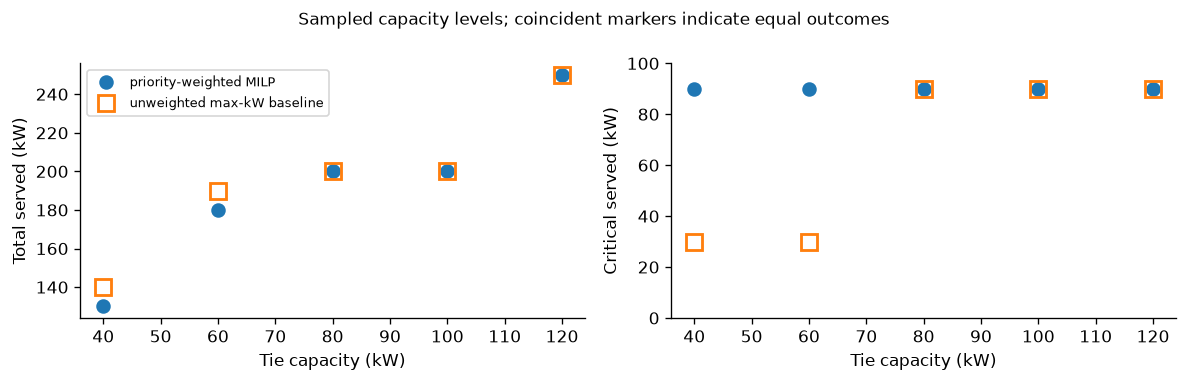
\includegraphics[width=\linewidth,height=3.65cm,keepaspectratio]{images/hands_on_L6_plot.png}
\par{\fontsize{7}{8.3}\selectfont\color{Slate} Reference L6 results. Both goals use the same network.}
\par\endgroup\smallskip
{
\small\begin{itemize}
\setlength{\itemsep}{.25em}
\item Critical-first goal: 130 kW total, including 90 kW for critical loads.
\item Most-total-power goal: 140 kW total, including 30 kW for critical loads.
\end{itemize}\par}
\vfill
{\fontsize{6.3}{7.5}\selectfont\color{Slate} Source: \href{https://colab.research.google.com/github/AlaaSelim-sudo/GridGuard-Agentic-AI-Tutorials/blob/main/agentic_grid_workflow_tutorial/Classroom_Labs.ipynb}{Classroom\_Labs.ipynb, L6; cell classroom-018; src/standard\_formulations.py.}\par}
\note{**Say**

Critical-first goal: 130 kW total, including 90 kW for critical loads. Most-total-power goal: 140 kW total, including 30 kW for critical loads. Read the 40 kW tie setting first. The left chart shows total service and the right shows critical service. The network is the same; the service goal changes the result.

**Show**

Use the actual source image. Point to the returned status or number that supports the slide's statement. State whether it is a fresh calculation or a saved example.

**Colab: NO NEW RUN**

Read the output from the previous run. Compare it with the reference figure; no new cell is needed.

Classroom Labs notebook. Classroom\_Labs.ipynb, L6; cell classroom-018; src/standard\_formulations.py. Public notebook and Python source. 24 October 2026; stable notebook cell IDs checked.
Full source: https://github.c\allowbreak{}om/AlaaSelim-sud\allowbreak{}o/GridGuard-Agen\allowbreak{}tic-AI-Tutorials\allowbreak{}/blob/main/agent\allowbreak{}ic\_grid\_workflow\allowbreak{}\_tutorial/Classr\allowbreak{}oom\_Labs.ipynb}
\end{frame}

\begin{frame}[t]{Check the restoration plan}
\relax
\begingroup\begin{minipage}[c][3.3cm][c]{\linewidth}\centering\setbox0=\hbox{\resizebox{.96\linewidth}{!}{\definecolor{Red}{HTML}{B83136}
\begin{tikzpicture}[x=1cm,y=1cm,font=\rmfamily\fontsize{12}{14}\selectfont,
 every node/.style={text=Navy,align=center},>=Latex,
 flow/.style={->,draw=IEEEBlue,line width=1.25pt},
 plainpoint/.style={circle,draw=IEEEBlue,fill=white,line width=1.25pt,minimum size=.55cm,inner sep=1pt}]

\node[plainpoint] (s0) at (0.8,1.6) {1};
\node[anchor=north,text width=3.1cm,font=\rmfamily\bfseries\fontsize{12}{14}\selectfont] at (0.8,1.08) {Fault stays isolated};
\node[anchor=north,text width=3.1cm,text=Slate,font=\rmfamily\fontsize{11}{13}\selectfont] at (0.8,-.35) {Unavailable branch};
\node[plainpoint] (s1) at (5.199999999999999,1.6) {2};
\node[anchor=north,text width=3.1cm,font=\rmfamily\bfseries\fontsize{12}{14}\selectfont] at (5.199999999999999,1.08) {Supply paths connect};
\node[anchor=north,text width=3.1cm,text=Slate,font=\rmfamily\fontsize{11}{13}\selectfont] at (5.199999999999999,-.35) {Restored loads};
\draw[flow] (s0)--(s1);
\node[plainpoint] (s2) at (9.6,1.6) {3};
\node[anchor=north,text width=3.1cm,font=\rmfamily\bfseries\fontsize{12}{14}\selectfont] at (9.6,1.08) {Capacity checks pass};
\node[anchor=north,text width=3.1cm,text=Slate,font=\rmfamily\fontsize{11}{13}\selectfont] at (9.6,-.35) {Within model limits};
\draw[flow] (s1)--(s2);
\node[plainpoint] (s3) at (13.999999999999998,1.6) {4};
\node[anchor=north,text width=3.1cm,font=\rmfamily\bfseries\fontsize{12}{14}\selectfont] at (13.999999999999998,1.08) {Report service};
\node[anchor=north,text width=3.1cm,text=Slate,font=\rmfamily\fontsize{11}{13}\selectfont] at (13.999999999999998,-.35) {Total and critical kW};
\draw[flow] (s2)--(s3);
\end{tikzpicture}
}}\ifdim\dimexpr\ht0+\dp0\relax>3.3cm\resizebox{!}{3.3cm}{\box0}\else\box0\fi\par\end{minipage}\par
{\fontsize{7}{8.3}\selectfont\color{Slate} Checks on the active-power model. AC and field-operation checks remain separate.\par}
\endgroup\smallskip
{
\small\begin{itemize}
\setlength{\itemsep}{.25em}
\item Keep the faulted branch out of service. Check supply paths and capacity.
\item Voltage, protection and field switching need separate studies.
\end{itemize}\par}
\vfill
{\fontsize{6.3}{7.5}\selectfont\color{Slate} Source: \href{https://colab.research.google.com/github/AlaaSelim-sudo/GridGuard-Agentic-AI-Tutorials/blob/main/agentic_grid_workflow_tutorial/Classroom_Labs.ipynb}{Classroom\_Labs.ipynb, L6; cell classroom-018; src/standard\_formulations.py.}\par}
\note{**Say**

Keep the faulted branch out of service. Check supply paths and capacity. Voltage, protection and field switching need separate studies. This small exercise uses an active-power service model. The agent can request and compare its results, while the operator must review the remaining work.

**Show**

Read the visual from the input to the result. Name the operator's goal, the agent's request and the fact supplied by the tool. Explain the decision in the two slide sentences.

**Colab: NO NEW RUN**

Explain the figure or discuss the output already produced. Do not run ahead.

Classroom Labs notebook. Classroom\_Labs.ipynb, L6; cell classroom-018; src/standard\_formulations.py. Public notebook and Python source. 24 October 2026; stable notebook cell IDs checked.
Full source: https://github.c\allowbreak{}om/AlaaSelim-sud\allowbreak{}o/GridGuard-Agen\allowbreak{}tic-AI-Tutorials\allowbreak{}/blob/main/agent\allowbreak{}ic\_grid\_workflow\allowbreak{}\_tutorial/Classr\allowbreak{}oom\_Labs.ipynb

Ying Wang, Yin Xu, Jiaxu Li, Jinghan He, Xiaojun Wang. On the Radiality Constraints for Distribution System Restoration and Reconfiguration Problems. Author preprint, arXiv:1912.05185v3. 15 March2020(v3); first submitted11 December2019.
Full source: https://arxiv.org/abs/1912.05185v3
Full paper: https://arxiv.org/pdf/1912.05185v3

Bo Chen, Chen Chen, Jianhui Wang, Karen L. Butler-Purry. Sequential Service Restoration for Unbalanced Distribution Systems and Microgrids. IEEE Transactions on Power Systems33(2),1507--1520. March2018.
Full source: https://doi.org/10.1109/TPWRS.2017.2720122}
\end{frame}

\begin{frame}[t]{Exercise 2: increase tie capacity}
\relax
\begingroup\fontsize{10}{13}\selectfont\ttfamily\raggedright
\noindent\strut\mbox{CAPACITIES\_KW~=~(40.,~60.,~80.,~100.,~120.,~180.)}\par
\endgroup\medskip
{
\normalsize\begin{itemize}
\item Add 180. to CAPACITIES\_KW. Keep 40. first. Predict, then rerun L6.
\item Compare total and critical power at 40 and 180 kW.
\item At which tested capacity do the two goals first give the same result?
\end{itemize}\par}
\vfill
{\fontsize{6.3}{7.5}\selectfont\color{Slate} Source: \href{https://colab.research.google.com/github/AlaaSelim-sudo/GridGuard-Agentic-AI-Tutorials/blob/main/agentic_grid_workflow_tutorial/Classroom_Labs.ipynb}{Classroom\_Labs.ipynb, L6; cell classroom-018; src/standard\_formulations.py.}\par}
\note{**Say**

Add 180. to CAPACITIES\_KW. Keep 40. first. Predict, then rerun L6. Compare total and critical power at 40 and 180 kW. At which tested capacity do the two goals first give the same result?

**Show**

Show the question for three minutes: predict for one, then edit and run for two. Advance once for the worked answer.

**Colab: EDIT AND RERUN**

Append 180. to CAPACITIES\_KW, keeping 40. first. Rerun all of L6. Give this exercise four minutes.

Exact cells: classroom-018. Run the whole cell, not only the slide excerpt.

**Expected result**

At 180 kW, both goals serve 250 kW total and 90 kW critical.

**Ask**

Add 180. to CAPACITIES\_KW. Keep 40. first. Predict, then rerun L6. Compare total and critical power at 40 and 180 kW. At which tested capacity do the two goals first give the same result?

**Answer**

At 40 kW, the priority goal serves 90 kW critical instead of 30 kW, with less total service. The goals first match at the tested 80 kW. At 180 kW, both serve 250 kW total and 90 kW critical. The goals first match at 80 kW among the tested capacities. At 180 kW both restore 250 kW total, including 90 kW critical. This discrete sweep does not identify an exact continuous crossover.

Classroom Labs notebook. Classroom\_Labs.ipynb, L6; cell classroom-018; src/standard\_formulations.py. Public notebook and Python source. 24 October 2026; stable notebook cell IDs checked.
Full source: https://github.c\allowbreak{}om/AlaaSelim-sud\allowbreak{}o/GridGuard-Agen\allowbreak{}tic-AI-Tutorials\allowbreak{}/blob/main/agent\allowbreak{}ic\_grid\_workflow\allowbreak{}\_tutorial/Classr\allowbreak{}oom\_Labs.ipynb}
\end{frame}

\begin{frame}[t]{Exercise 2 answer: capacity changes the trade-off}
\relax
\begingroup\begin{minipage}[c][3.3cm][c]{\linewidth}\centering\setbox0=\hbox{\resizebox{.96\linewidth}{!}{\definecolor{Red}{HTML}{B83136}
\begin{tikzpicture}[font=\rmfamily\fontsize{11}{13}\selectfont,x=.029cm,y=1cm]
\node[anchor=west,font=\rmfamily\bfseries\fontsize{13}{15}\selectfont] at (-90,4.0) {Service restored: critical + other demand};
\fill[Cyan] (28,3.48) rectangle (39,3.65);\node[anchor=west] at (44,3.56) {Critical kW};
\fill[IEEEBlue!40] (127,3.48) rectangle (138,3.65);\node[anchor=west] at (143,3.56) {Other served kW};
\node[anchor=east,align=right] at (-4,2.91) {40 kW tie\\Weighted};
\node[anchor=east] at (-4,2.2) {Max-kW};
\node[anchor=east,align=right] at (-4,1.15) {180 kW tie\\Weighted};
\node[anchor=east] at (-4,.44) {Max-kW};
\fill[Cyan] (0,2.7) rectangle (90,3.12);\fill[IEEEBlue!40] (90,2.7) rectangle (130,3.12);
\fill[Cyan] (0,1.99) rectangle (30,2.41);\fill[IEEEBlue!40] (30,1.99) rectangle (140,2.41);
\fill[Cyan] (0,.94) rectangle (90,1.36);\fill[IEEEBlue!40] (90,.94) rectangle (250,1.36);
\fill[Cyan] (0,.23) rectangle (90,.65);\fill[IEEEBlue!40] (90,.23) rectangle (250,.65);
\node at (45,2.91) {90};\node at (15,2.2) {30};\node at (45,1.15) {90};\node at (45,.44) {90};
\node[anchor=west] at (134,2.91) {130 total};\node[anchor=west] at (144,2.2) {140 total};
\node[anchor=west] at (254,1.15) {250 total};\node[anchor=west] at (254,.44) {250 total};
\draw[->,Slate] (0,0)--(285,0);\foreach \x in {0,50,100,150,200,250}{\draw[Slate] (\x,0)--(\x,-.06) node[below] {\x};}
\end{tikzpicture}
}}\ifdim\dimexpr\ht0+\dp0\relax>3.3cm\resizebox{!}{3.3cm}{\box0}\else\box0\fi\par\end{minipage}\par
{\fontsize{7}{8.3}\selectfont\color{Slate} Fresh L6 results. Cyan shows critical service; blue shows other service.\par}
\endgroup\smallskip
{
\small\begin{itemize}
\setlength{\itemsep}{.25em}
\item At 40 kW, the priority goal serves 90 kW critical instead of 30 kW, with less total service.
\item The goals first match at the tested 80 kW. At 180 kW, both serve 250 kW total and 90 kW critical.
\end{itemize}\par}
\vfill
{\fontsize{6.3}{7.5}\selectfont\color{Slate} Source: \href{https://colab.research.google.com/github/AlaaSelim-sudo/GridGuard-Agentic-AI-Tutorials/blob/main/agentic_grid_workflow_tutorial/Classroom_Labs.ipynb}{Classroom\_Labs.ipynb, L6; cell classroom-018; fresh MILP and exhaustive-check sweep.}\par}
\note{**Say**

At 40 kW, the priority goal serves 90 kW critical instead of 30 kW, with less total service. The goals first match at the tested 80 kW. At 180 kW, both serve 250 kW total and 90 kW critical. The goals first match at 80 kW among the tested capacities. At 180 kW both restore 250 kW total, including 90 kW critical. This discrete sweep does not identify an exact continuous crossover.

**Show**

Advance from the exercise only after learners try it. Read the verified values, explain why the outcome occurs and answer every part of the question.

**Colab: INSPECT / RESET**

Use the exercise output. Keep 40 first; restore the original list and rerun L6 before L7.

**Expected result**

At 40 kW, priorities give more critical service: 90 kW instead of 30 kW, with less total service. The goals match from 80 kW in the tested list. At 180 kW, both serve 250 kW total, including 90 kW critical.

Classroom Labs notebook. Classroom\_Labs.ipynb, L6; cell classroom-018; src/standard\_formulations.py. Public notebook and Python source. 24 October 2026; stable notebook cell IDs checked.
Full source: https://github.c\allowbreak{}om/AlaaSelim-sud\allowbreak{}o/GridGuard-Agen\allowbreak{}tic-AI-Tutorials\allowbreak{}/blob/main/agent\allowbreak{}ic\_grid\_workflow\allowbreak{}\_tutorial/Classr\allowbreak{}oom\_Labs.ipynb}
\end{frame}

\begin{frame}[t]{A changed request needs a new check}
\relax
{\fontsize{8}{10}\selectfont\color{Slate} Run the whole cell in Colab\par}\smallskip
\lstinputlisting[basicstyle=\ttfamily\fontsize{12}{14.5}\selectfont,aboveskip=3pt,belowskip=10pt,breaklines=true,gobble=0]{../research/code/restoration_Classroom_Labs_classroom-021_L8-9.py}
{
\small\begin{itemize}
\setlength{\itemsep}{.25em}
\item Restore the original capacity list and rerun L6.
\item Run L7: the requested capacity changes from 40 kW to 20 kW.
\end{itemize}\par}
\vfill
{\fontsize{6.3}{7.5}\selectfont\color{Slate} Source: \href{https://colab.research.google.com/github/AlaaSelim-sudo/GridGuard-Agentic-AI-Tutorials/blob/main/agentic_grid_workflow_tutorial/Classroom_Labs.ipynb}{Classroom\_Labs.ipynb, L7; cell classroom-021; request/evidence binding.}\par}
\note{**Say**

Restore the original capacity list and rerun L6. Run L7: the requested capacity changes from 40 kW to 20 kW. Run the complete L7 cell after restoring L6. It compares an old checked result with a request that now has a smaller capacity.

**Show**

Locate L7 in Classroom Labs. Show the highlighted source lines, then run the whole cell when the Colab cue says to run. Read the returned result in plain words.

**Colab: RESET, THEN RUN**

Restore the original capacity list and rerun L6. Then run the whole L7 cell.

Exact cells: classroom-018, classroom-021. Run the whole cell, not only the slide excerpt.

**Expected result**

Original contract: True. Changed rating with old evidence: False. HOLD requests a fresh solve.

Classroom Labs notebook. Classroom\_Labs.ipynb, L7; cell classroom-021; request/evidence binding. Public notebook and Python source. 24 October 2026; stable notebook cell IDs checked.
Full source: https://github.c\allowbreak{}om/AlaaSelim-sud\allowbreak{}o/GridGuard-Agen\allowbreak{}tic-AI-Tutorials\allowbreak{}/blob/main/agent\allowbreak{}ic\_grid\_workflow\allowbreak{}\_tutorial/Classr\allowbreak{}oom\_Labs.ipynb}
\end{frame}

\begin{frame}[t]{A new limit needs a new study}
\relax
\begingroup\begin{minipage}[c][3.3cm][c]{\linewidth}\centering\setbox0=\hbox{\resizebox{.96\linewidth}{!}{\definecolor{Red}{HTML}{B83136}
\begin{tikzpicture}[x=1cm,y=1cm,font=\rmfamily\fontsize{12}{14}\selectfont,
 every node/.style={text=Navy,align=center},>=Latex,
 flow/.style={->,draw=IEEEBlue,line width=1.25pt},
 plainpoint/.style={circle,draw=IEEEBlue,fill=white,line width=1.25pt,minimum size=.55cm,inner sep=1pt}]

\node[text width=3.3cm] at (1.4,2.2) {Old request\\40 kW capacity};
\node[text width=3.5cm] at (7,2.2) {Matching old study};
\node[text=Cyan,font=\rmfamily\bfseries] at (12.5,2.2) {Can be reviewed};
\draw[flow] (3.3,2.2)--(5,2.2);\draw[flow] (9,2.2)--(10.8,2.2);
\node[text width=3.5cm] at (1.4,.2) {Changed request\\20 kW capacity};
\node[text width=3.5cm] at (7,.2) {Same old study};
\node[text=Red,text width=3.7cm,font=\rmfamily\bfseries] at (12.5,.2) {HOLD\\Request a new solve};
\draw[flow] (3.3,.2)--(5,.2);\draw[flow,draw=Red] (9,.2)--(10.8,.2);

\end{tikzpicture}
}}\ifdim\dimexpr\ht0+\dp0\relax>3.3cm\resizebox{!}{3.3cm}{\box0}\else\box0\fi\par\end{minipage}\par
{\fontsize{7}{8.3}\selectfont\color{Slate} A failed input match asks for a new study; it does not establish physical infeasibility.\par}
\endgroup\smallskip
{
\small\begin{itemize}
\setlength{\itemsep}{.25em}
\item The original request matches the old result. The changed request does not.
\item Hold the old proposal, calculate again and check the new result.
\end{itemize}\par}
\vfill
{\fontsize{6.3}{7.5}\selectfont\color{Slate} Source: \href{https://colab.research.google.com/github/AlaaSelim-sudo/GridGuard-Agentic-AI-Tutorials/blob/main/agentic_grid_workflow_tutorial/Classroom_Labs.ipynb}{Classroom\_Labs.ipynb, L7; cell classroom-021; request/evidence binding.}\par}
\note{**Say**

The original request matches the old result. The changed request does not. Hold the old proposal, calculate again and check the new result. The two L7 match tests return True and False. This tests whether evidence belongs to the request; it does not prove that a new plan is physically feasible.

**Show**

Read the visual from the input to the result. Name the operator's goal, the agent's request and the fact supplied by the tool. Explain the decision in the two slide sentences.

**Colab: NO NEW RUN**

Explain the figure or discuss the output already produced. Do not run ahead.

Classroom Labs notebook. Classroom\_Labs.ipynb, L7; cell classroom-021; request/evidence binding. Public notebook and Python source. 24 October 2026; stable notebook cell IDs checked.
Full source: https://github.c\allowbreak{}om/AlaaSelim-sud\allowbreak{}o/GridGuard-Agen\allowbreak{}tic-AI-Tutorials\allowbreak{}/blob/main/agent\allowbreak{}ic\_grid\_workflow\allowbreak{}\_tutorial/Classr\allowbreak{}oom\_Labs.ipynb}
\end{frame}

\begin{frame}[t]{The agent keeps the operator's goal}
\relax
\begingroup\begin{minipage}[c][3.25cm][c]{\linewidth}\centering\setbox0=\hbox{\resizebox{.96\linewidth}{!}{\begingroup
\hyphenpenalty=10000\exhyphenpenalty=10000
\definecolor{IEEEBlue}{HTML}{00629B}
\definecolor{Cyan}{HTML}{00A6B2}
\definecolor{Navy}{HTML}{003B5C}
\definecolor{Slate}{HTML}{526470}
\definecolor{RestRed}{HTML}{B83136}
\definecolor{RestAmber}{HTML}{A66610}
\begin{tikzpicture}[x=.90cm,y=.82cm,font=\fontsize{11}{12}\selectfont,
  every node/.style={text=Navy},
  flow/.style={-{Stealth[length=2mm]},line width=1pt,draw=IEEEBlue},
  bus/.style={circle,draw=IEEEBlue,line width=1pt,minimum size=5.5mm,inner sep=1pt,fill=white},
  textblock/.style={align=center,inner sep=1pt},
  pass/.style={draw=Cyan,line width=2pt},
  available/.style={draw=Slate,line width=.8pt},
  optional/.style={draw=RestAmber,dashed,line width=1pt}]
\begin{scope}[x=.88cm]
\node[bus] (r0) at (0.8,1.55) {0};
\node[bus] (r1) at (2.8,2.3) {1};
\node[bus,draw=RestAmber] (r2) at (5.5,2.3) {2};
\node[bus] (r3) at (8.1,1.55) {3};
\node[bus] (r4) at (5.5,.55) {4};
\node[bus,draw=RestAmber] (r5) at (2.8,.55) {5};
\draw[available] (r0)--(r1);
\draw[RestRed,dashed,line width=1.4pt] (r1)--(r2);
\node[text=RestRed,fill=white] at (3.45,1.86) {fault open};
\draw[available] (r2)--(r3)--(r4);
\draw[available] (r2)--(r5);
\draw[optional] (r1)--node[left=1mm,fill=white,text=RestAmber] {100 kW}(r5);
\draw[optional] (r0) to[out=-60,in=200] (r4);
\node[anchor=west,text=RestAmber] at (.2,-.5) {tie 0--4: 40 kW};
\node[above=1mm of r1] {40 kW};
\node[above=1mm of r2,text=RestAmber] {60 kW critical};
\node[above=1mm of r3] {70 kW};
\node[right=1mm of r4] {50 kW};
\node[anchor=west,text=RestAmber] at (3.3,-.15) {30 kW critical};
\node[left=1mm of r0] {source};
\draw[pass] (r0)--(r1)--(r5)--(r2);
\node[bus,fill=Cyan!20] at (0.8,1.55) {0};
\node[bus,fill=Cyan!20] at (2.8,2.3) {1};
\node[bus,draw=RestAmber,fill=RestAmber!15] at (5.5,2.3) {2};
\node[bus,draw=RestAmber,fill=RestAmber!15] at (2.8,.55) {5};
\node[textblock,text width=2.8cm] at (10.9,2.1) {Picked up: 1, 2, 5\\130 kW total};
\node[textblock,text width=3.2cm,text=RestAmber] at (10.9,.45) {Critical service\\90 kW};
\end{scope}
\end{tikzpicture}
\endgroup
}}\ifdim\dimexpr\ht0+\dp0\relax>3.25cm\resizebox{!}{3.25cm}{\box0}\else\box0\fi\par\end{minipage}\par
{\fontsize{7}{8.3}\selectfont\color{Slate} Proposed agent use. L6 itself runs Python.\par}
\endgroup\smallskip
{
\small\begin{itemize}
\setlength{\itemsep}{.25em}
\item The operator sets priorities. The solver selects loads.
\item The agent can request the solve and explain the returned service trade-off.
\end{itemize}\par}
\vfill
{\fontsize{6.3}{7.5}\selectfont\color{Slate} Source: \href{https://colab.research.google.com/github/AlaaSelim-sudo/GridGuard-Agentic-AI-Tutorials/blob/main/agentic_grid_workflow_tutorial/Classroom_Labs.ipynb}{Classroom\_Labs.ipynb, L6; cell classroom-018; src/standard\_formulations.py.}\par}
\note{**Say**

The operator sets priorities. The solver selects loads. The agent can request the solve and explain the returned service trade-off. Keeping the goal fixed matters when many studies are requested. The agent should return the achieved total and critical service with each result.

**Show**

Use the two short slide statements to explain the idea. Link it to the operator's next decision or to the named Colab cell.

**Colab: PREVIEW ONLY**

Show the slide only. Run L6 later on slide 37; keep the notebook in order.

**Expected result**

No new notebook output on this slide.

Classroom Labs notebook. Classroom\_Labs.ipynb, L6; cell classroom-018; src/standard\_formulations.py. Public notebook and Python source. 24 October 2026; stable notebook cell IDs checked.
Full source: https://github.c\allowbreak{}om/AlaaSelim-sud\allowbreak{}o/GridGuard-Agen\allowbreak{}tic-AI-Tutorials\allowbreak{}/blob/main/agent\allowbreak{}ic\_grid\_workflow\allowbreak{}\_tutorial/Classr\allowbreak{}oom\_Labs.ipynb}
\end{frame}

\begin{frame}[t]{Recorded example: try more service}
\relax
\begingroup\centering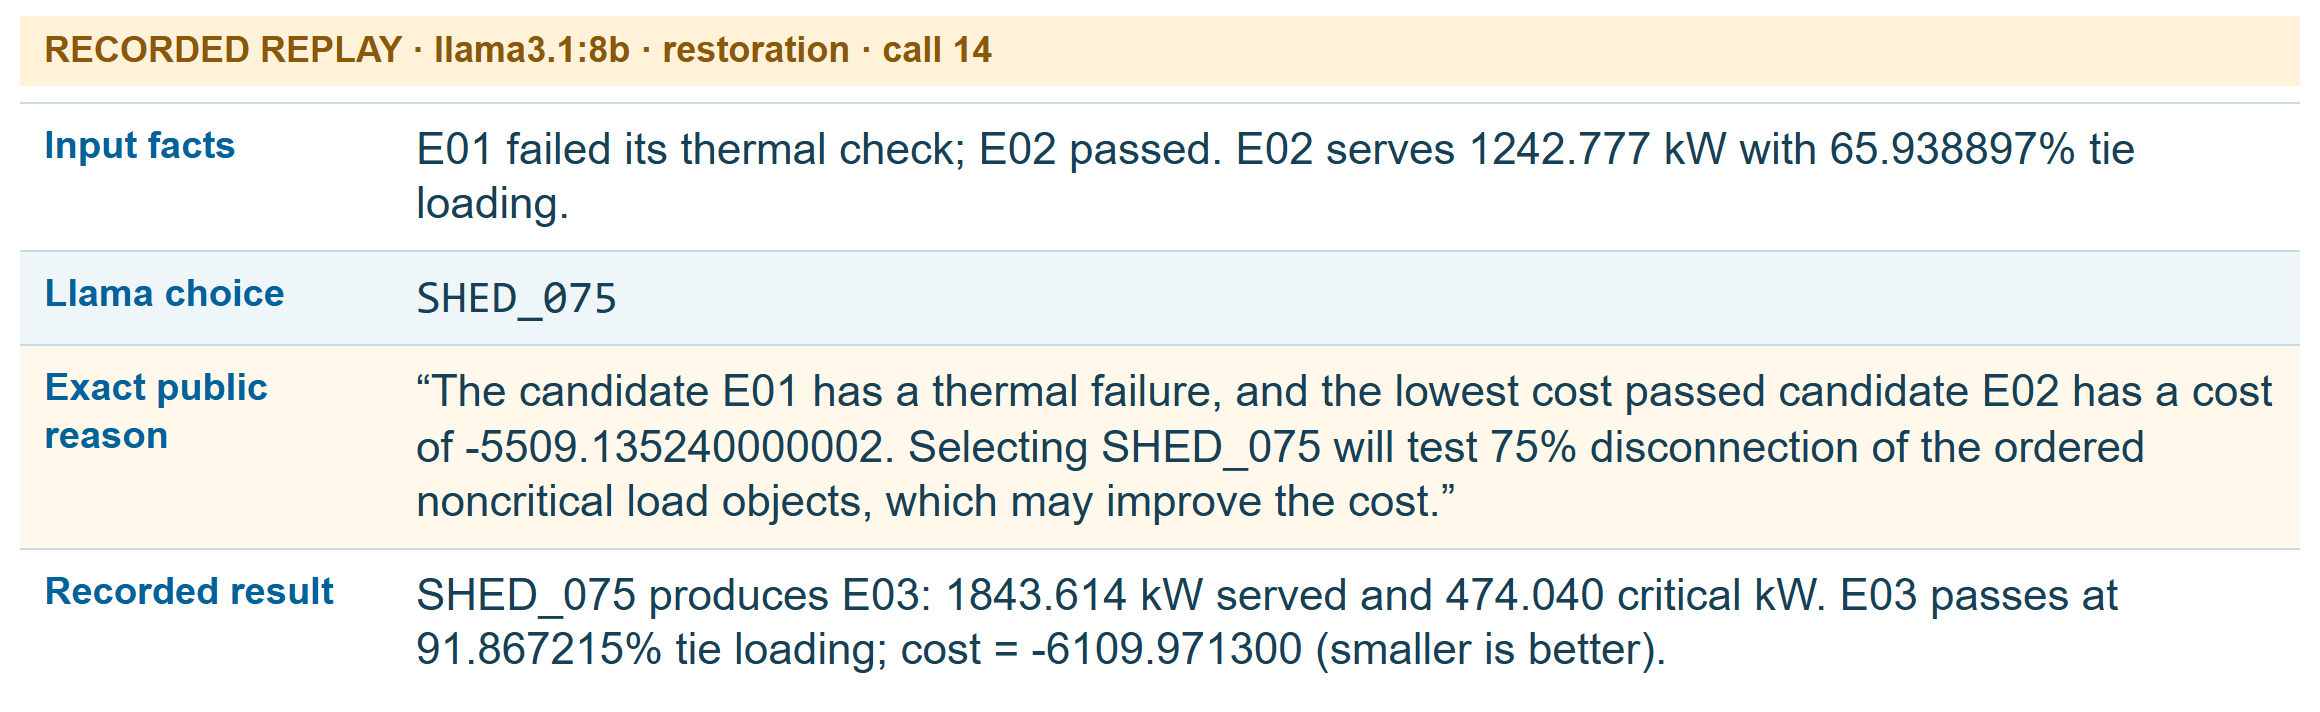
\includegraphics[width=\linewidth,height=4cm,keepaspectratio]{images/llama_restoration_14.png}
\par\endgroup\smallskip
{
\small\begin{itemize}
\setlength{\itemsep}{.25em}
\item This saved feeder study is different from L6.
\item Llama requests another plan. The tool reports more service and passing checks.
\end{itemize}\par}
\vfill
{\fontsize{6.3}{7.5}\selectfont\color{Slate} Source: \href{https://colab.research.google.com/github/AlaaSelim-sudo/GridGuard-Agentic-AI-Tutorials/blob/main/agentic_grid_workflow_tutorial/Classroom_Labs.ipynb}{Classroom Labs L10B: restoration replay, recorded call 14; full record in source guide.}\par}
\note{**Say**

This saved feeder study is different from L6. Llama requests another plan. The tool reports more service and passing checks. The saved feeder example is larger than the L6 exercise and has different numbers. Watch the request, returned check and next choice rather than comparing its total kW with L6.

**Show**

Preview the actual saved Llama request and returned tool evidence. Do not ask learners to run ahead. L10B will replay these records after the three labs.

**Colab: PREVIEW ONLY**

Show the slide only. Run L10B later on slide 64; keep the notebook in order.

**Expected result**

No new notebook output on this slide.

Workshop recorded model replies and numerical study records. Feeder-catalog restoration: Llama 3.1:8b refinement and ranking calls 14--16. Public teaching archive. 27 September 2026.
Full source: https://github.c\allowbreak{}om/AlaaSelim-sud\allowbreak{}o/GridGuard-Agen\allowbreak{}tic-AI-Tutorials\allowbreak{}/blob/main/agent\allowbreak{}ic\_grid\_workflow\allowbreak{}\_tutorial/result\allowbreak{}s/proposal\_run\_2\allowbreak{}0260927T184402Z\_\allowbreak{}53e0cf/llama\_cal\allowbreak{}ls.json

Classroom Labs notebook and Python helper. L10B: Watch how Llama chooses a tool; src/llama\_walkthrough.py. Public reproducible teaching material. 24 October 2026.
Full source: https://github.c\allowbreak{}om/AlaaSelim-sud\allowbreak{}o/GridGuard-Agen\allowbreak{}tic-AI-Tutorials\allowbreak{}/blob/main/agent\allowbreak{}ic\_grid\_workflow\allowbreak{}\_tutorial/src/ll\allowbreak{}ama\_walkthrough.\allowbreak{}py}
\end{frame}

\begin{frame}[t]{Recorded example: the tool rejects a trial}
\relax
\begingroup\centering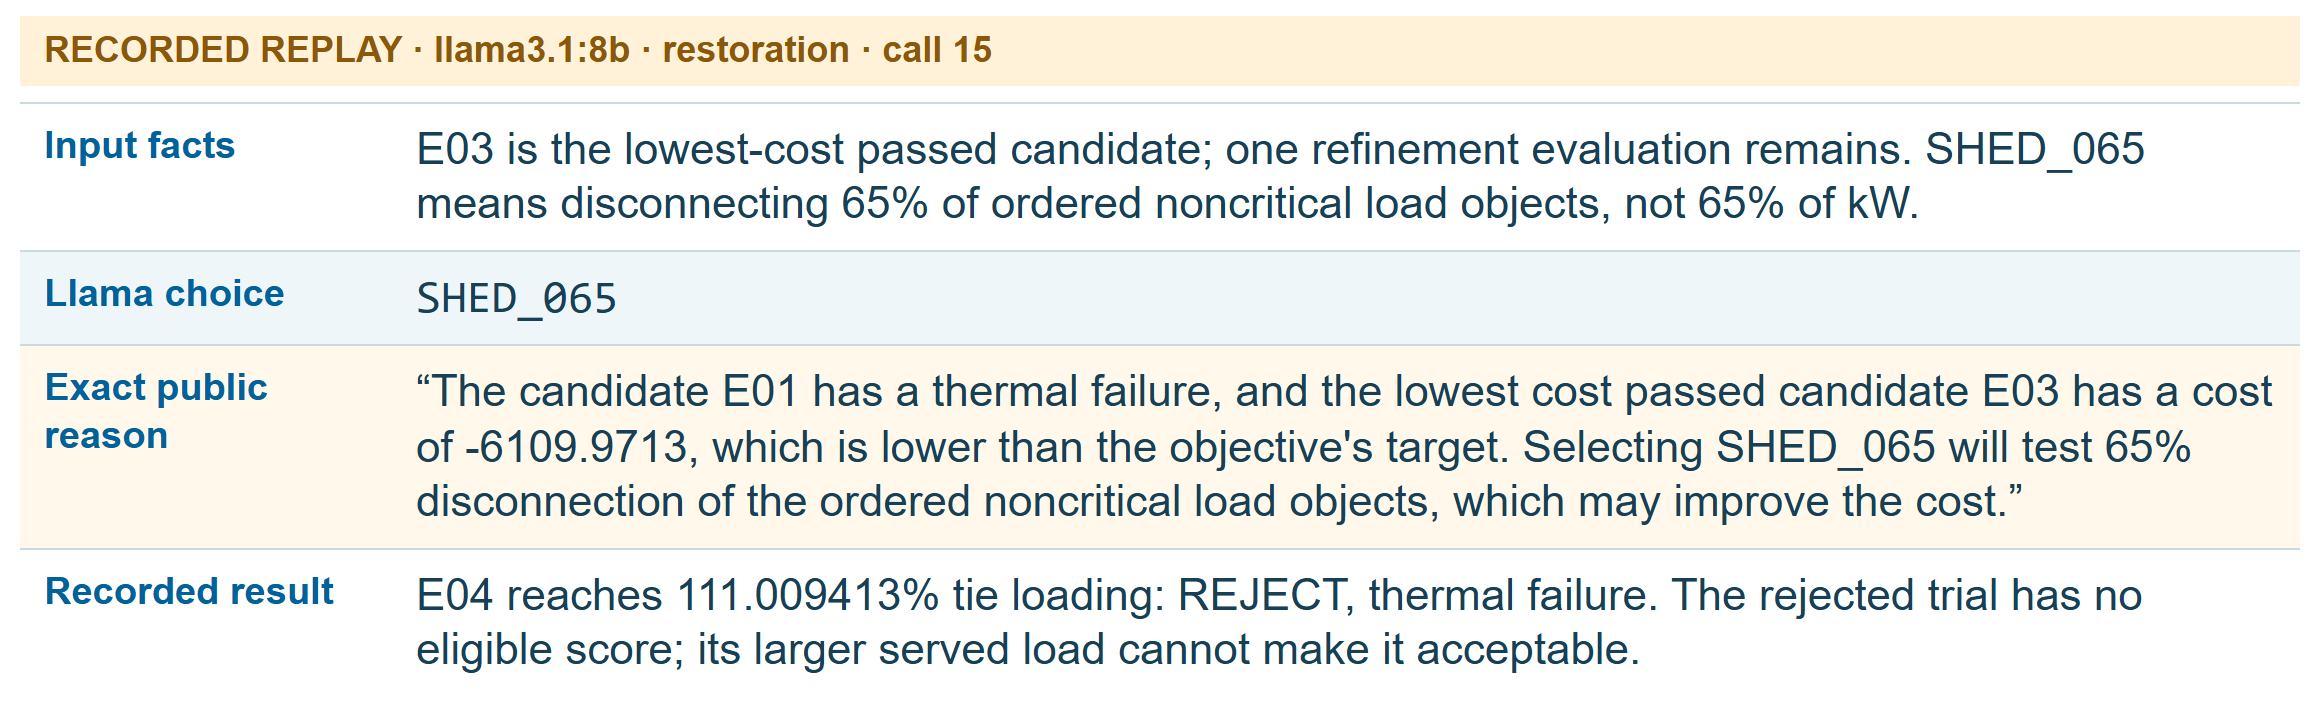
\includegraphics[width=\linewidth,height=4cm,keepaspectratio]{images/llama_restoration_15.png}
\par\endgroup\smallskip
{
\small\begin{itemize}
\setlength{\itemsep}{.25em}
\item The next trial carries too much current.
\item It cannot replace the previous passing option.
\end{itemize}\par}
\vfill
{\fontsize{6.3}{7.5}\selectfont\color{Slate} Source: \href{https://colab.research.google.com/github/AlaaSelim-sudo/GridGuard-Agentic-AI-Tutorials/blob/main/agentic_grid_workflow_tutorial/Classroom_Labs.ipynb}{Classroom Labs L10B: restoration replay, recorded call 15; full record in source guide.}\par}
\note{**Say**

The next trial carries too much current. It cannot replace the previous passing option. The numerical guard excludes the overloaded trial. Restoring more load is useful only when the required checks also pass.

**Show**

Preview the actual saved Llama request and returned tool evidence. Do not ask learners to run ahead. L10B will replay these records after the three labs.

**Colab: PREVIEW ONLY**

Show the slide only. Run L10B later on slide 64; keep the notebook in order.

**Expected result**

No new notebook output on this slide.

Workshop recorded model replies and numerical study records. Feeder-catalog restoration: Llama 3.1:8b refinement and ranking calls 14--16. Public teaching archive. 27 September 2026.
Full source: https://github.c\allowbreak{}om/AlaaSelim-sud\allowbreak{}o/GridGuard-Agen\allowbreak{}tic-AI-Tutorials\allowbreak{}/blob/main/agent\allowbreak{}ic\_grid\_workflow\allowbreak{}\_tutorial/result\allowbreak{}s/proposal\_run\_2\allowbreak{}0260927T184402Z\_\allowbreak{}53e0cf/llama\_cal\allowbreak{}ls.json

Classroom Labs notebook and Python helper. L10B: Watch how Llama chooses a tool; src/llama\_walkthrough.py. Public reproducible teaching material. 24 October 2026.
Full source: https://github.c\allowbreak{}om/AlaaSelim-sud\allowbreak{}o/GridGuard-Agen\allowbreak{}tic-AI-Tutorials\allowbreak{}/blob/main/agent\allowbreak{}ic\_grid\_workflow\allowbreak{}\_tutorial/src/ll\allowbreak{}ama\_walkthrough.\allowbreak{}py}
\end{frame}

\begin{frame}[t]{Recorded example: correct a wrong ranking}
\relax
\begingroup\centering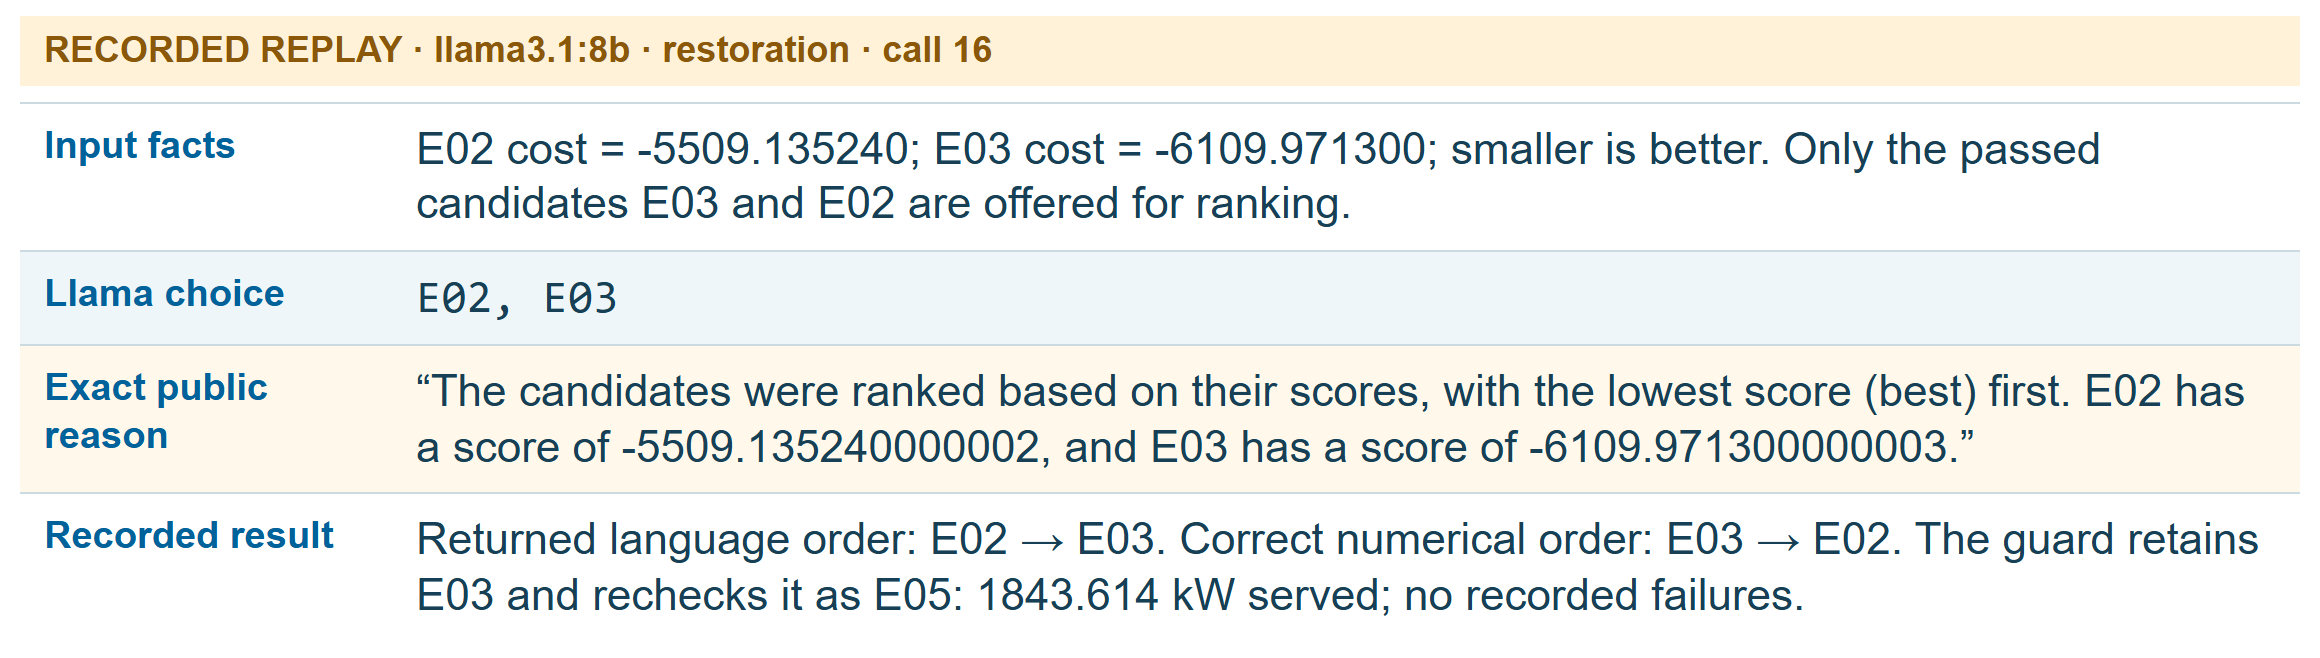
\includegraphics[width=\linewidth,height=4cm,keepaspectratio]{images/llama_restoration_16.png}
\par\endgroup\smallskip
{
\small\begin{itemize}
\setlength{\itemsep}{.25em}
\item Llama puts two passing plans in the wrong order.
\item Python keeps the lower-cost plan and checks it again.
\end{itemize}\par}
\vfill
{\fontsize{6.3}{7.5}\selectfont\color{Slate} Source: \href{https://colab.research.google.com/github/AlaaSelim-sudo/GridGuard-Agentic-AI-Tutorials/blob/main/agentic_grid_workflow_tutorial/Classroom_Labs.ipynb}{Classroom Labs L10B: restoration replay, recorded call 16; full record in source guide.}\par}
\note{**Say**

Llama puts two passing plans in the wrong order. Python keeps the lower-cost plan and checks it again. Here the lower costs are negative: about minus 6109 is lower than minus 5509. The model's order is wrong, so Python corrects it and rechecks the retained plan.

**Show**

Preview the actual saved Llama request and returned tool evidence. Do not ask learners to run ahead. L10B will replay these records after the three labs.

**Colab: PREVIEW ONLY**

Show the slide only. Run L10B later on slide 64; keep the notebook in order.

**Expected result**

No new notebook output on this slide.

Workshop recorded model replies and numerical study records. Feeder-catalog restoration: Llama 3.1:8b refinement and ranking calls 14--16. Public teaching archive. 27 September 2026.
Full source: https://github.c\allowbreak{}om/AlaaSelim-sud\allowbreak{}o/GridGuard-Agen\allowbreak{}tic-AI-Tutorials\allowbreak{}/blob/main/agent\allowbreak{}ic\_grid\_workflow\allowbreak{}\_tutorial/result\allowbreak{}s/proposal\_run\_2\allowbreak{}0260927T184402Z\_\allowbreak{}53e0cf/llama\_cal\allowbreak{}ls.json

Classroom Labs notebook and Python helper. L10B: Watch how Llama chooses a tool; src/llama\_walkthrough.py. Public reproducible teaching material. 24 October 2026.
Full source: https://github.c\allowbreak{}om/AlaaSelim-sud\allowbreak{}o/GridGuard-Agen\allowbreak{}tic-AI-Tutorials\allowbreak{}/blob/main/agent\allowbreak{}ic\_grid\_workflow\allowbreak{}\_tutorial/src/ll\allowbreak{}ama\_walkthrough.\allowbreak{}py}
\end{frame}

\begin{frame}[t]{Case 3: can we trust these readings?}
\relax
\begingroup\begin{minipage}[c][3.3cm][c]{\linewidth}\centering\setbox0=\hbox{\resizebox{.96\linewidth}{!}{\definecolor{Red}{HTML}{B83136}
\begin{tikzpicture}[x=1cm,y=1cm,font=\rmfamily\fontsize{12}{14}\selectfont,
 every node/.style={text=Navy,align=center},>=Latex,
 flow/.style={->,draw=IEEEBlue,line width=1.25pt},
 plainpoint/.style={circle,draw=IEEEBlue,fill=white,line width=1.25pt,minimum size=.55cm,inner sep=1pt}]

\node[text=Red,anchor=west] at (0,3) {Some readings may be wrong};
\node[plainpoint] (a) at (1.5,1.6) {1};\node[below=.3cm of a,text width=3.2cm] {Meter readings};
\node[plainpoint] (b) at (7,1.6) {?};\node[below=.3cm of b,text width=3.2cm] {Fit the grid model};
\node[plainpoint,draw=Red] (c) at (12.5,1.6) {?};\node[below=.3cm of c,text width=3.2cm] {Trust these\\readings?};
\draw[flow] (a)--(b);\draw[flow] (b)--node[above] {Looks consistent}(c);
\node[text=Red,font=\rmfamily\bfseries] at (7,-.25) {A good fit is not the same as true data};

\end{tikzpicture}
}}\ifdim\dimexpr\ht0+\dp0\relax>3.3cm\resizebox{!}{3.3cm}{\box0}\else\box0\fi\par\end{minipage}\par
{\fontsize{7}{8.3}\selectfont\color{Slate} Concept sketch. L8 uses a small four-bus DC model.\par}
\endgroup\smallskip
{
\small\begin{itemize}
\setlength{\itemsep}{.25em}
\item Wrong readings can still look consistent with the model.
\item The agent can request checks, but action still needs a trusted basis.
\end{itemize}\par}
\vfill
{\fontsize{6.3}{7.5}\selectfont\color{Slate} Source: \href{https://colab.research.google.com/github/AlaaSelim-sudo/GridGuard-Agentic-AI-Tutorials/blob/main/agentic_grid_workflow_tutorial/Classroom_Labs.ipynb}{Classroom\_Labs.ipynb, L8; cell classroom-023; four-bus DC fixture.}\par}
\note{**Say**

The operator sees measurements, not the true system state. Several altered readings can agree with each other and still lead to a wrong estimate. An agent can request tests and organize the evidence, but it cannot create a trusted measurement source. The lab uses known simulated changes so that we can compare fit with actual estimation error.

**Show**

Read the visual from the input to the result. Name the operator's goal, the agent's request and the fact supplied by the tool. Explain the decision in the two slide sentences.

**Colab: PREVIEW ONLY**

Show the slide only. Run L8 later on slide 51; keep the notebook in order.

**Expected result**

No new notebook output on this slide.

**Ask**

Does a good fit prove a reading is true?

**Answer**

No. Coordinated wrong readings can fit the model while giving a wrong estimated state.

Classroom Labs notebook. Classroom\_Labs.ipynb, L8; cell classroom-023; four-bus DC fixture. Public notebook and Python source. 24 October 2026; stable notebook cell IDs checked.
Full source: https://github.c\allowbreak{}om/AlaaSelim-sud\allowbreak{}o/GridGuard-Agen\allowbreak{}tic-AI-Tutorials\allowbreak{}/blob/main/agent\allowbreak{}ic\_grid\_workflow\allowbreak{}\_tutorial/Classr\allowbreak{}oom\_Labs.ipynb}
\end{frame}

\begin{frame}[t]{How the agent helps with suspicious readings}
\relax
\begingroup\begin{minipage}[c][3.3cm][c]{\linewidth}\centering\setbox0=\hbox{\resizebox{.96\linewidth}{!}{\definecolor{Red}{HTML}{B83136}
\begin{tikzpicture}[x=1cm,y=1cm,font=\rmfamily\fontsize{12}{14}\selectfont,
 every node/.style={text=Navy,align=center},>=Latex,
 flow/.style={->,draw=IEEEBlue,line width=1.25pt},
 plainpoint/.style={circle,draw=IEEEBlue,fill=white,line width=1.25pt,minimum size=.55cm,inner sep=1pt}]

\node[plainpoint] (s0) at (0.8,1.6) {1};
\node[anchor=north,text width=3.1cm,font=\rmfamily\bfseries\fontsize{12}{14}\selectfont] at (0.8,1.08) {Read the\\inputs};
\node[anchor=north,text width=3.1cm,text=Slate,font=\rmfamily\fontsize{11}{13}\selectfont] at (0.8,-.35) {Readings\\and trust};
\node[plainpoint] (s1) at (4.1,1.6) {2};
\node[anchor=north,text width=3.1cm,font=\rmfamily\bfseries\fontsize{12}{14}\selectfont] at (4.1,1.08) {Agent\\requests};
\node[anchor=north,text width=3.1cm,text=Slate,font=\rmfamily\fontsize{11}{13}\selectfont] at (4.1,-.35) {Permitted\\study};
\draw[flow] (s0)--(s1);
\node[plainpoint] (s2) at (7.3999999999999995,1.6) {3};
\node[anchor=north,text width=3.1cm,font=\rmfamily\bfseries\fontsize{12}{14}\selectfont] at (7.3999999999999995,1.08) {Tool\\calculates};
\node[anchor=north,text width=3.1cm,text=Slate,font=\rmfamily\fontsize{11}{13}\selectfont] at (7.3999999999999995,-.35) {Estimate and\\correction};
\draw[flow] (s1)--(s2);
\node[plainpoint] (s3) at (10.7,1.6) {4};
\node[anchor=north,text width=3.1cm,font=\rmfamily\bfseries\fontsize{12}{14}\selectfont] at (10.7,1.08) {Check the\\conditions};
\node[anchor=north,text width=3.1cm,text=Slate,font=\rmfamily\fontsize{11}{13}\selectfont] at (10.7,-.35) {HOLD if\\evidence missing};
\draw[flow] (s2)--(s3);
\node[plainpoint] (s4) at (14.0,1.6) {5};
\node[anchor=north,text width=3.1cm,font=\rmfamily\bfseries\fontsize{12}{14}\selectfont] at (14.0,1.08) {Operator\\reviews};
\node[anchor=north,text width=3.1cm,text=Slate,font=\rmfamily\fontsize{11}{13}\selectfont] at (14.0,-.35) {Choose the\\next step};
\draw[flow] (s3)--(s4);
\draw[flow,draw=Cyan] (s3.north) -- ++(0,.9) -| node[pos=.25,above,text=Cyan] {Use the result to choose the next trial} (s1.north);
\end{tikzpicture}
}}\ifdim\dimexpr\ht0+\dp0\relax>3.3cm\resizebox{!}{3.3cm}{\box0}\else\box0\fi\par\end{minipage}\par
{\fontsize{7}{8.3}\selectfont\color{Slate} Concept map. L9 calculates; L10B replays saved Llama requests and returned tool evidence.\par}
\endgroup\smallskip
{
\small\begin{itemize}
\setlength{\itemsep}{.25em}
\item The agent can request the checks and keep missing evidence visible.
\item The operator reviews trust, model coverage and the proposed correction.
\end{itemize}\par}
\vfill
{\fontsize{6.3}{7.5}\selectfont\color{Slate} Source: \href{https://colab.research.google.com/github/AlaaSelim-sudo/GridGuard-Agentic-AI-Tutorials/blob/main/agentic_grid_workflow_tutorial/Classroom_Labs.ipynb}{Classroom\_Labs.ipynb, L9; cell classroom-026; fixed trusted-recovery fixture.}\par}
\note{**Say**

Follow the information from the readings to the proposed correction. Without the required trusted data, the workflow returns HOLD. With that assumption, the tool can calculate a candidate. The agent can request these steps and explain missing checks; the operator must still assess the premise and decide the authorized next step.

**Show**

Read the visual from the input to the result. Name the operator's goal, the agent's request and the fact supplied by the tool. Explain the decision in the two slide sentences.

**Colab: NO NEW RUN**

Read the output from the previous run. Compare it with the reference figure; no new cell is needed.

Classroom Labs notebook. Classroom\_Labs.ipynb, L9; cell classroom-026; fixed trusted-recovery fixture. Public notebook and Python source. 24 October 2026; stable notebook cell IDs checked.
Full source: https://github.c\allowbreak{}om/AlaaSelim-sud\allowbreak{}o/GridGuard-Agen\allowbreak{}tic-AI-Tutorials\allowbreak{}/blob/main/agent\allowbreak{}ic\_grid\_workflow\allowbreak{}\_tutorial/Classr\allowbreak{}oom\_Labs.ipynb}
\end{frame}

\begin{frame}[t]{Mismatch is only one check}
\relax
\begingroup\begin{minipage}[c][3.3cm][c]{\linewidth}\centering\setbox0=\hbox{\resizebox{.96\linewidth}{!}{\definecolor{Red}{HTML}{B83136}
\begin{tikzpicture}[x=1cm,y=1cm,font=\rmfamily\fontsize{12}{14}\selectfont,
 every node/.style={text=Navy,align=center},>=Latex,
 flow/.style={->,draw=IEEEBlue,line width=1.25pt},
 plainpoint/.style={circle,draw=IEEEBlue,fill=white,line width=1.25pt,minimum size=.55cm,inner sep=1pt}]

\node[anchor=west,font=\rmfamily\bfseries] at (0,3.1) {Mismatch score $J$};
\fill[Red!8] (10.05,.7) rectangle (13,2.35);
\draw[->,Slate,thick] (1,1.2)--(13.4,1.2);
\foreach \x/\v in {1/0,4/5,7/10,10/15,13/20}{\draw[Slate] (\x,1.12)--(\x,1.28);\node[below] at (\x,1.05) {\v};}
\draw[Red,thick] (10.05,.65)--(10.05,2.4);\node[above,text=Red] at (10.05,2.4) {Alarm threshold 15.09};
\fill[IEEEBlue] (3.352,1.2) circle (.1);\node[above,text width=3.8cm] at (3.35,1.65) {Example: 3.92\\Below the threshold};
\node[text=Slate] at (7,-.25) {A low mismatch does not authenticate a reading};

\end{tikzpicture}
}}\ifdim\dimexpr\ht0+\dp0\relax>3.3cm\resizebox{!}{3.3cm}{\box0}\else\box0\fi\par\end{minipage}\par
{\fontsize{7}{8.3}\selectfont\color{Slate} Mismatch J here has a different meaning from control cost J in the voltage lab.\par}
\endgroup\smallskip
{
\small\begin{itemize}
\setlength{\itemsep}{.25em}
\item Mismatch J measures how well the model fits the readings.
\item The simulation lets us measure how wrong the estimate is (state error).
\end{itemize}\par}
\vfill
{\fontsize{6.3}{7.5}\selectfont\color{Slate} Source: \href{https://colab.research.google.com/github/AlaaSelim-sudo/GridGuard-Agentic-AI-Tutorials/blob/main/agentic_grid_workflow_tutorial/Classroom_Labs.ipynb}{Classroom\_Labs.ipynb, L8; cell classroom-023; four-bus DC fixture.}\par}
\note{**Say**

Mismatch J measures how well the model fits the readings. The simulation lets us measure how wrong the estimate is (state error). In the cyber lab, J is a mismatch statistic, not the control cost used in the voltage lab. A low mismatch says the model fits the readings; it does not authenticate them.

**Show**

Read the visual from the input to the result. Name the operator's goal, the agent's request and the fact supplied by the tool. Explain the decision in the two slide sentences.

**Colab: PREVIEW ONLY**

Show the slide only. Run L8 later on slide 51; keep the notebook in order.

**Expected result**

No new notebook output on this slide.

**Ask**

What does a low mismatch tell us?

**Answer**

That the model fits the supplied readings, not that the readings are authentic.

Classroom Labs notebook. Classroom\_Labs.ipynb, L8; cell classroom-023; four-bus DC fixture. Public notebook and Python source. 24 October 2026; stable notebook cell IDs checked.
Full source: https://github.c\allowbreak{}om/AlaaSelim-sud\allowbreak{}o/GridGuard-Agen\allowbreak{}tic-AI-Tutorials\allowbreak{}/blob/main/agent\allowbreak{}ic\_grid\_workflow\allowbreak{}\_tutorial/Classr\allowbreak{}oom\_Labs.ipynb

Fred C. Schweppe, J. Wildes. Power System Static-State Estimation, Part I: Exact Model. IEEE Transactions on Power Apparatus and Systems, PAS-89(1), pp. 120--125. January 1970.
Full source: https://doi.org/10.1109/TPAS.1970.292678}
\end{frame}

\begin{frame}[t]{Two ways readings can be misleading}
\relax
{\fontsize{8}{10}\selectfont\color{Slate} Run the whole cell in Colab\par}\smallskip
\lstinputlisting[basicstyle=\ttfamily\fontsize{12}{14.5}\selectfont,aboveskip=3pt,belowskip=10pt,breaklines=true,gobble=0]{../research/code/cyber_Classroom_Labs_classroom-023_L1-3.py}
{
\small\begin{itemize}
\setlength{\itemsep}{.25em}
\item Run L8 with the default settings.
\item Compare one biased reading with a coordinated change across several readings.
\end{itemize}\par}
\vfill
{\fontsize{6.3}{7.5}\selectfont\color{Slate} Source: \href{https://colab.research.google.com/github/AlaaSelim-sudo/GridGuard-Agentic-AI-Tutorials/blob/main/agentic_grid_workflow_tutorial/Classroom_Labs.ipynb}{Classroom\_Labs.ipynb, L8; cell classroom-023; four-bus DC fixture.}\par}
\note{**Say**

Run L8 with the default settings. Compare one biased reading with a coordinated change across several readings. The isolated pattern changes one reading. The coordinated pattern changes several together. We compare the same two questions: did the alarm trigger, and how wrong was the estimated state?

**Show**

Locate L8 in Classroom Labs. Show the highlighted source lines, then run the whole cell when the Colab cue says to run. Read the returned result in plain words.

**Colab: RUN**

Run L8 with ATTACK\_SCALES=(0.,.25,.5,1.,1.5).

Exact cells: classroom-023. Run the whole cell, not only the slide excerpt.

**Expected result**

A coordinated Hc attack preserves a small residual while offline state error grows.

Classroom Labs notebook. Classroom\_Labs.ipynb, L8; cell classroom-023; four-bus DC fixture. Public notebook and Python source. 24 October 2026; stable notebook cell IDs checked.
Full source: https://github.c\allowbreak{}om/AlaaSelim-sud\allowbreak{}o/GridGuard-Agen\allowbreak{}tic-AI-Tutorials\allowbreak{}/blob/main/agent\allowbreak{}ic\_grid\_workflow\allowbreak{}\_tutorial/Classr\allowbreak{}oom\_Labs.ipynb}
\end{frame}

\begin{frame}[t]{Read the alarm and the estimation error}
\relax
\begingroup\centering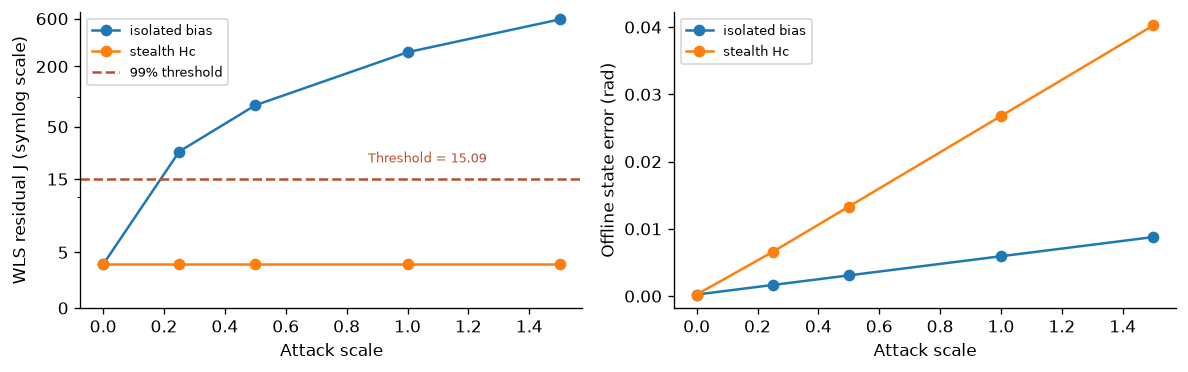
\includegraphics[width=\linewidth,height=3.65cm,keepaspectratio]{images/hands_on_L8_plot.png}
\par{\fontsize{7}{8.3}\selectfont\color{Slate} Reference L8 plots: model fit and estimation error are different checks.}
\par\endgroup\smallskip
{
\small\begin{itemize}
\setlength{\itemsep}{.25em}
\item Left: mismatch and its alarm threshold. Right: error against the simulation's known truth.
\item A quiet alarm can appear alongside a growing error.
\end{itemize}\par}
\vfill
{\fontsize{6.3}{7.5}\selectfont\color{Slate} Source: \href{https://colab.research.google.com/github/AlaaSelim-sudo/GridGuard-Agentic-AI-Tutorials/blob/main/agentic_grid_workflow_tutorial/Classroom_Labs.ipynb}{Classroom\_Labs.ipynb, L8; cell classroom-023; four-bus DC fixture.}\par}
\note{**Say**

Left: mismatch and its alarm threshold. Right: error against the simulation's known truth. A quiet alarm can appear alongside a growing error. The right plot uses truth known inside the simulation. A real operator usually cannot read that error directly from a live system.

**Show**

Use the actual source image. Point to the returned status or number that supports the slide's statement. State whether it is a fresh calculation or a saved example.

**Colab: NO NEW RUN**

Read the output from the previous run. Compare it with the reference figure; no new cell is needed.

Classroom Labs notebook. Classroom\_Labs.ipynb, L8; cell classroom-023; four-bus DC fixture. Public notebook and Python source. 24 October 2026; stable notebook cell IDs checked.
Full source: https://github.c\allowbreak{}om/AlaaSelim-sud\allowbreak{}o/GridGuard-Agen\allowbreak{}tic-AI-Tutorials\allowbreak{}/blob/main/agent\allowbreak{}ic\_grid\_workflow\allowbreak{}\_tutorial/Classr\allowbreak{}oom\_Labs.ipynb}
\end{frame}

\begin{frame}[t]{A coordinated change can escape the alarm}
\relax
\begingroup\begin{minipage}[c][3.3cm][c]{\linewidth}\centering\setbox0=\hbox{\resizebox{.96\linewidth}{!}{\definecolor{Red}{HTML}{B83136}
\begin{tikzpicture}[x=1cm,y=1cm,font=\rmfamily\fontsize{12}{14}\selectfont,
 every node/.style={text=Navy,align=center},>=Latex,
 flow/.style={->,draw=IEEEBlue,line width=1.25pt},
 plainpoint/.style={circle,draw=IEEEBlue,fill=white,line width=1.25pt,minimum size=.55cm,inner sep=1pt}]

\node[font=\rmfamily\bfseries] at (3.2,3.1) {One biased reading};\node[font=\rmfamily\bfseries] at (10.9,3.1) {Coordinated change};
\node[font=\rmfamily\bfseries\fontsize{20}{23}\selectfont,text=Red] at (3.2,2) {$J=277.50$};
\node[font=\rmfamily\bfseries\fontsize{20}{23}\selectfont,text=IEEEBlue] at (10.9,2) {$J=3.92$};
\draw[flow,draw=Red] (3.2,1.45)--(3.2,.65);\draw[flow] (10.9,1.45)--(10.9,.65);
\node[text=Red,font=\rmfamily\bfseries] at (3.2,.25) {Alarm};
\node[font=\rmfamily\bfseries] at (10.9,.25) {No alarm};
\node[text=Slate,text width=6cm] at (10.9,-.55) {State error: 0.02678 rad\\The estimate is still wrong};

\end{tikzpicture}
}}\ifdim\dimexpr\ht0+\dp0\relax>3.3cm\resizebox{!}{3.3cm}{\box0}\else\box0\fi\par\end{minipage}\par
{\fontsize{7}{8.3}\selectfont\color{Slate} L8 reference values at attack scale 1. Simulation truth supplies the state error.\par}
\endgroup\smallskip
{
\small\begin{itemize}
\setlength{\itemsep}{.25em}
\item At scale 1, one biased reading gives mismatch J=277.50 and an alarm.
\item A coordinated change gives J=3.92, no alarm, and 0.02678 rad of state error.
\end{itemize}\par}
\vfill
{\fontsize{6.3}{7.5}\selectfont\color{Slate} Source: \href{https://colab.research.google.com/github/AlaaSelim-sudo/GridGuard-Agentic-AI-Tutorials/blob/main/agentic_grid_workflow_tutorial/Classroom_Labs.ipynb}{Classroom\_Labs.ipynb, L8; cell classroom-023; four-bus DC fixture.}\par}
\note{**Say**

At scale 1, one biased reading gives mismatch J=277.50 and an alarm. A coordinated change gives J=3.92, no alarm, and 0.02678 rad of state error. The coordinated changes preserve a small mismatch even as the estimate moves away from the known state. This is the reason a quiet alarm is incomplete evidence.

**Show**

Read the visual from the input to the result. Name the operator's goal, the agent's request and the fact supplied by the tool. Explain the decision in the two slide sentences.

**Colab: NO NEW RUN**

Read the output from the previous run. Compare it with the reference figure; no new cell is needed.

Classroom Labs notebook. Classroom\_Labs.ipynb, L8; cell classroom-023; four-bus DC fixture. Public notebook and Python source. 24 October 2026; stable notebook cell IDs checked.
Full source: https://github.c\allowbreak{}om/AlaaSelim-sud\allowbreak{}o/GridGuard-Agen\allowbreak{}tic-AI-Tutorials\allowbreak{}/blob/main/agent\allowbreak{}ic\_grid\_workflow\allowbreak{}\_tutorial/Classr\allowbreak{}oom\_Labs.ipynb

Yao Liu, Peng Ning, Michael K. Reiter. False Data Injection Attacks against State Estimation in Electric Power Grids. ACM Transactions on Information and System Security, 14(1), Article 13, 33 pages. May 2011.
Full source: https://doi.org/10.1145/1952982.1952995
Full paper: https://reitermk\allowbreak{}.github.io/paper\allowbreak{}s/2011/TISSEC2.p\allowbreak{}df}
\end{frame}

\begin{frame}[t]{Exercise 3: test a small bias}
\relax
\begingroup\fontsize{10}{13}\selectfont\ttfamily\raggedright
\noindent\strut\mbox{ATTACK\_SCALES~=~(0.,~.10,~.25,~.5,~1.,~1.5)}\par
\endgroup\medskip
{
\normalsize\begin{itemize}
\item Add .10 to ATTACK\_SCALES. Predict, then rerun L8.
\item At scale 0.10, compare mismatch J, the alarm and state error.
\item Does no alarm prove that the readings are correct?
\end{itemize}\par}
\vfill
{\fontsize{6.3}{7.5}\selectfont\color{Slate} Source: \href{https://colab.research.google.com/github/AlaaSelim-sudo/GridGuard-Agentic-AI-Tutorials/blob/main/agentic_grid_workflow_tutorial/Classroom_Labs.ipynb}{Classroom\_Labs.ipynb, L8; cell classroom-023; four-bus DC fixture.}\par}
\note{**Say**

Add .10 to ATTACK\_SCALES. Predict, then rerun L8. At scale 0.10, compare mismatch J, the alarm and state error. Does no alarm prove that the readings are correct?

**Show**

Show the question for three minutes: predict for one, then edit and run for two. Advance once for the worked answer.

**Colab: EDIT AND RERUN**

Add .10 to ATTACK\_SCALES. Rerun all of L8 and inspect the isolated-bias row. Give this exercise four minutes.

Exact cells: classroom-023. Run the whole cell, not only the slide excerpt.

**Expected result**

At isolated scale 0.10, J is about 10.14, below the 15.09 threshold; no alarm is not proof of truth.

**Ask**

Add .10 to ATTACK\_SCALES. Predict, then rerun L8. At scale 0.10, compare mismatch J, the alarm and state error. Does no alarm prove that the readings are correct?

**Answer**

Both alarms are False at scale 0.10, but both estimates still have error. No alarm means the mismatch is below this threshold. It does not establish data trust. At scale 0.10, the isolated mismatch is about 10.143 and the coordinated mismatch is about 3.920. Both are below 15.086, while their state errors are nonzero.

Classroom Labs notebook. Classroom\_Labs.ipynb, L8; cell classroom-023; four-bus DC fixture. Public notebook and Python source. 24 October 2026; stable notebook cell IDs checked.
Full source: https://github.c\allowbreak{}om/AlaaSelim-sud\allowbreak{}o/GridGuard-Agen\allowbreak{}tic-AI-Tutorials\allowbreak{}/blob/main/agent\allowbreak{}ic\_grid\_workflow\allowbreak{}\_tutorial/Classr\allowbreak{}oom\_Labs.ipynb}
\end{frame}

\begin{frame}[t]{Exercise 3 answer: no alarm can hide an error}
\relax
\begingroup\begin{minipage}[c][3.3cm][c]{\linewidth}\centering\setbox0=\hbox{\resizebox{.96\linewidth}{!}{\definecolor{Red}{HTML}{B83136}
\begin{tikzpicture}[font=\rmfamily\fontsize{12}{14}\selectfont,x=.56cm,y=1cm]
\node[anchor=west,font=\rmfamily\bfseries\fontsize{13}{15}\selectfont] at (-5.6,3.0) {Residual test at attack scale 0.10};
\draw[->,Slate] (0,0)--(18,0);\foreach \x in {0,5,10,15}{\draw[Slate] (\x,0)--(\x,-.08) node[below] {\x};}
\draw[Red,dashed,thick] (15.086272,.15)--(15.086272,2.1) node[above,text=Red] {alarm threshold 15.086};
\fill[IEEEBlue] (0,1.5) rectangle (10.143237,1.93);\fill[Cyan] (0,.5) rectangle (3.920222,.93);
\node[anchor=east,align=right] at (-.5,1.72) {Isolated bias};
\node[anchor=east,align=right] at (-.5,.72) {Coordinated $Hc$};
\node[anchor=west,font=\rmfamily\bfseries\fontsize{12}{14}\selectfont] at (10.4,1.72) {$J=10.143$};
\node[anchor=west,font=\rmfamily\bfseries\fontsize{12}{14}\selectfont] at (4.2,.72) {$J=3.920$};
\node[anchor=west,text=Slate] at (0,1.23) {alarm = False / state error 0.000806 rad};
\node[anchor=west,text=Slate] at (0,.23) {alarm = False / state error 0.002553 rad};
\end{tikzpicture}
}}\ifdim\dimexpr\ht0+\dp0\relax>3.3cm\resizebox{!}{3.3cm}{\box0}\else\box0\fi\par\end{minipage}\par
{\fontsize{7}{8.3}\selectfont\color{Slate} Fresh L8 exercise. The error uses truth known inside the simulation.\par}
\endgroup\smallskip
{
\small\begin{itemize}
\setlength{\itemsep}{.25em}
\item Both alarms are False at scale 0.10, but both estimates still have error.
\item No alarm means the mismatch is below this threshold. It does not establish data trust.
\end{itemize}\par}
\vfill
{\fontsize{6.3}{7.5}\selectfont\color{Slate} Source: \href{https://colab.research.google.com/github/AlaaSelim-sudo/GridGuard-Agentic-AI-Tutorials/blob/main/agentic_grid_workflow_tutorial/Classroom_Labs.ipynb}{Classroom\_Labs.ipynb, L8; cell classroom-023; fresh four-bus DC residual check at scale 0.10.}\par}
\note{**Say**

Both alarms are False at scale 0.10, but both estimates still have error. No alarm means the mismatch is below this threshold. It does not establish data trust. At scale 0.10, the isolated mismatch is about 10.143 and the coordinated mismatch is about 3.920. Both are below 15.086, while their state errors are nonzero.

**Show**

Advance from the exercise only after learners try it. Read the verified values, explain why the outcome occurs and answer every part of the question.

**Colab: INSPECT / RESET**

Use the output already produced for the exercise. Restore the original ATTACK\_SCALES and rerun L8 before the separate fixed L9 recovery case.

**Expected result**

At scale 0.10, both alarms are False. Both state estimates still have error; the coordinated shift has the larger error here. No alarm means J is below this threshold. It does not prove correct data or trusted sensors.

Classroom Labs notebook. Classroom\_Labs.ipynb, L8; cell classroom-023; four-bus DC fixture. Public notebook and Python source. 24 October 2026; stable notebook cell IDs checked.
Full source: https://github.c\allowbreak{}om/AlaaSelim-sud\allowbreak{}o/GridGuard-Agen\allowbreak{}tic-AI-Tutorials\allowbreak{}/blob/main/agent\allowbreak{}ic\_grid\_workflow\allowbreak{}\_tutorial/Classr\allowbreak{}oom\_Labs.ipynb}
\end{frame}

\begin{frame}[t]{Back to the original data-bias settings}
\relax
{\fontsize{8}{10}\selectfont\color{Slate} Run the whole cell in Colab\par}\smallskip
\lstinputlisting[basicstyle=\ttfamily\fontsize{12}{14.5}\selectfont,aboveskip=3pt,belowskip=10pt,breaklines=true,gobble=0]{../research/code/cyber_Classroom_Labs_classroom-023_L1-3.py}
{
\small\begin{itemize}
\setlength{\itemsep}{.25em}
\item Restore the original attack scales and rerun L8.
\item L9 uses a separate fixed recovery case.
\end{itemize}\par}
\vfill
{\fontsize{6.3}{7.5}\selectfont\color{Slate} Source: \href{https://colab.research.google.com/github/AlaaSelim-sudo/GridGuard-Agentic-AI-Tutorials/blob/main/agentic_grid_workflow_tutorial/Classroom_Labs.ipynb}{Classroom\_Labs.ipynb, L8; cell classroom-023; four-bus DC fixture.}\par}
\note{**Say**

Restore the original attack scales and rerun L8. L9 uses a separate fixed recovery case. L9 is deliberately a fixed recovery example. Your L8 sweep is a separate experiment and does not select the L9 correction.

**Show**

Locate L8 in Classroom Labs. Show the highlighted source lines, then run the whole cell when the Colab cue says to run. Read the returned result in plain words.

**Colab: RESET AND RERUN**

Restore ATTACK\_SCALES=(0.,.25,.5,1.,1.5) and rerun all of L8.

Exact cells: classroom-023. Run the whole cell, not only the slide excerpt.

**Expected result**

The default sweep returns. L9 remains a separate fixed recovery fixture.

Classroom Labs notebook. Classroom\_Labs.ipynb, L8; cell classroom-023; four-bus DC fixture. Public notebook and Python source. 24 October 2026; stable notebook cell IDs checked.
Full source: https://github.c\allowbreak{}om/AlaaSelim-sud\allowbreak{}o/GridGuard-Agen\allowbreak{}tic-AI-Tutorials\allowbreak{}/blob/main/agent\allowbreak{}ic\_grid\_workflow\allowbreak{}\_tutorial/Classr\allowbreak{}oom\_Labs.ipynb}
\end{frame}

\begin{frame}[t]{Trusted readings must come from somewhere}
\relax
\begingroup\begin{minipage}[c][3.3cm][c]{\linewidth}\centering\setbox0=\hbox{\resizebox{.96\linewidth}{!}{\definecolor{Red}{HTML}{B83136}
\begin{tikzpicture}[x=1cm,y=1cm,font=\rmfamily\fontsize{12}{14}\selectfont,
 every node/.style={text=Navy,align=center},>=Latex,
 flow/.style={->,draw=IEEEBlue,line width=1.25pt},
 plainpoint/.style={circle,draw=IEEEBlue,fill=white,line width=1.25pt,minimum size=.55cm,inner sep=1pt}]

\node[font=\rmfamily\bfseries,text width=5cm] (q) at (1.7,1.5) {Are the required trusted\\readings assumed available?};
\node[text=Red,font=\rmfamily\bfseries] (hold) at (10.5,2.7) {HOLD};
\node[font=\rmfamily\bfseries] (study) at (10.5,.2) {Calculate a proposal};
\draw[flow,draw=Red] (4.4,1.65)-|node[pos=.3,above,text=Red] {No}(hold.west);
\draw[flow] (4.4,1.35)-|node[pos=.3,below] {Yes}(study.west);
\node[text=Slate,text width=7cm] at (8,-.75) {The example supplies this premise.\\The calculation does not prove data trust.};

\end{tikzpicture}
}}\ifdim\dimexpr\ht0+\dp0\relax>3.3cm\resizebox{!}{3.3cm}{\box0}\else\box0\fi\par\end{minipage}\par
{\fontsize{7}{8.3}\selectfont\color{Slate} The extra readings are assumed trustworthy for this experiment.\par}
\endgroup\smallskip
{
\small\begin{itemize}
\setlength{\itemsep}{.25em}
\item This example assumes extra trustworthy readings are available.
\item Neither the fitting tool nor Llama proves that these readings are authentic.
\end{itemize}\par}
\vfill
{\fontsize{6.3}{7.5}\selectfont\color{Slate} Source: \href{https://colab.research.google.com/github/AlaaSelim-sudo/GridGuard-Agentic-AI-Tutorials/blob/main/agentic_grid_workflow_tutorial/Classroom_Labs.ipynb}{Classroom\_Labs.ipynb, L9; cell classroom-026; fixed trusted-recovery fixture.}\par}
\note{**Say**

This example assumes extra trustworthy readings are available. Neither the fitting tool nor Llama proves that these readings are authentic. The lesson supplies a trust assumption so that the numerical task can be studied. The calculation is not a method for proving sensor identity or integrity.

**Show**

Read the visual from the input to the result. Name the operator's goal, the agent's request and the fact supplied by the tool. Explain the decision in the two slide sentences.

**Colab: PREVIEW ONLY**

Show the slide only. Run L9 later on slide 58; keep the notebook in order.

**Expected result**

No new notebook output on this slide.

**Ask**

Does Llama authenticate the extra readings?

**Answer**

No. Their trustworthiness is an explicit assumption of this example.

Classroom Labs notebook. Classroom\_Labs.ipynb, L9; cell classroom-026; fixed trusted-recovery fixture. Public notebook and Python source. 24 October 2026; stable notebook cell IDs checked.
Full source: https://github.c\allowbreak{}om/AlaaSelim-sud\allowbreak{}o/GridGuard-Agen\allowbreak{}tic-AI-Tutorials\allowbreak{}/blob/main/agent\allowbreak{}ic\_grid\_workflow\allowbreak{}\_tutorial/Classr\allowbreak{}oom\_Labs.ipynb}
\end{frame}

\begin{frame}[t]{Does the result say HOLD or PROPOSE?}
\relax
{\fontsize{8}{10}\selectfont\color{Slate} Run the whole cell in Colab\par}\smallskip
\lstinputlisting[basicstyle=\ttfamily\fontsize{12}{14.5}\selectfont,aboveskip=3pt,belowskip=10pt,breaklines=true,gobble=0]{../research/code/cyber_Classroom_Labs_classroom-026_L1-2.py}
{
\small\begin{itemize}
\setlength{\itemsep}{.25em}
\item Run L9 and read the status before the proposed adjustment.
\item Then check the model's returned limits and remaining assumptions.
\end{itemize}\par}
\vfill
{\fontsize{6.3}{7.5}\selectfont\color{Slate} Source: \href{https://colab.research.google.com/github/AlaaSelim-sudo/GridGuard-Agentic-AI-Tutorials/blob/main/agentic_grid_workflow_tutorial/Classroom_Labs.ipynb}{Classroom\_Labs.ipynb, L9; cell classroom-026; fixed trusted-recovery fixture.}\par}
\note{**Say**

Run L9 and read the status before the proposed adjustment. Then check the model's returned limits and remaining assumptions. HOLD means a required condition is absent. PROPOSE means the tool can offer a model-based correction for review, not permission to operate equipment.

**Show**

Locate L9 in Classroom Labs. Show the highlighted source lines, then run the whole cell when the Colab cue says to run. Read the returned result in plain words.

**Colab: RUN**

Run all of L9 after resetting L8.

Exact cells: classroom-026. Run the whole cell, not only the slide excerpt.

**Expected result**

No trusted replacement readings: HOLD. With assumed trusted readings: PROPOSE, u about 0.121694 p.u., zero offline violations.

Classroom Labs notebook. Classroom\_Labs.ipynb, L9; cell classroom-026; fixed trusted-recovery fixture. Public notebook and Python source. 24 October 2026; stable notebook cell IDs checked.
Full source: https://github.c\allowbreak{}om/AlaaSelim-sud\allowbreak{}o/GridGuard-Agen\allowbreak{}tic-AI-Tutorials\allowbreak{}/blob/main/agent\allowbreak{}ic\_grid\_workflow\allowbreak{}\_tutorial/Classr\allowbreak{}oom\_Labs.ipynb}
\end{frame}

\begin{frame}[t]{Missing trust means HOLD}
\relax
\begingroup\centering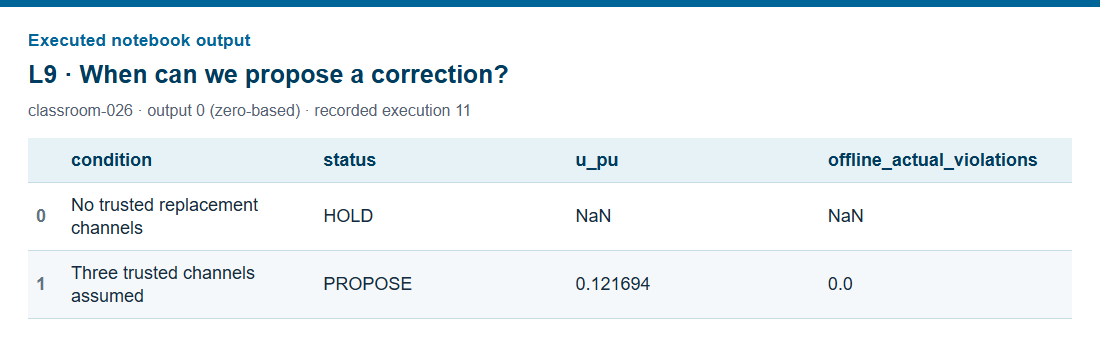
\includegraphics[width=\linewidth,height=3.3cm,keepaspectratio]{images/hands_on_L9_trust.png}
\par{\fontsize{7}{8.3}\selectfont\color{Slate} Reference L9 output for the fixed recovery example.}
\par\endgroup\smallskip
{
\small\begin{itemize}
\setlength{\itemsep}{.25em}
\item Without trusted replacement readings: HOLD.
\item With the trust assumption: PROPOSE a 0.121694 p.u. adjustment; the offline model checks pass.
\end{itemize}\par}
\vfill
{\fontsize{6.3}{7.5}\selectfont\color{Slate} Source: \href{https://colab.research.google.com/github/AlaaSelim-sudo/GridGuard-Agentic-AI-Tutorials/blob/main/agentic_grid_workflow_tutorial/Classroom_Labs.ipynb}{Classroom\_Labs.ipynb, L9; cell classroom-026; fixed trusted-recovery fixture.}\par}
\note{**Say**

Without trusted replacement readings: HOLD. With the trust assumption: PROPOSE a 0.121694 p.u. adjustment; the offline model checks pass. The passing result depends on the declared trust premise and the simplified model. Zero offline violations is a model result, not a field guarantee.

**Show**

Use the actual source image. Point to the returned status or number that supports the slide's statement. State whether it is a fresh calculation or a saved example.

**Colab: NO NEW RUN**

Read the output from the previous run. Compare it with the reference figure; no new cell is needed.

Classroom Labs notebook. Classroom\_Labs.ipynb, L9; cell classroom-026; fixed trusted-recovery fixture. Public notebook and Python source. 24 October 2026; stable notebook cell IDs checked.
Full source: https://github.c\allowbreak{}om/AlaaSelim-sud\allowbreak{}o/GridGuard-Agen\allowbreak{}tic-AI-Tutorials\allowbreak{}/blob/main/agent\allowbreak{}ic\_grid\_workflow\allowbreak{}\_tutorial/Classr\allowbreak{}oom\_Labs.ipynb}
\end{frame}

\begin{frame}[t]{The tool calculates a small correction}
\relax
\begingroup\begin{minipage}[c][3.3cm][c]{\linewidth}\centering\setbox0=\hbox{\resizebox{.96\linewidth}{!}{\definecolor{Red}{HTML}{B83136}
\begin{tikzpicture}[x=1cm,y=1cm,font=\rmfamily\fontsize{12}{14}\selectfont,
 every node/.style={text=Navy,align=center},>=Latex,
 flow/.style={->,draw=IEEEBlue,line width=1.25pt},
 plainpoint/.style={circle,draw=IEEEBlue,fill=white,line width=1.25pt,minimum size=.55cm,inner sep=1pt}]

\node[anchor=west,font=\rmfamily\bfseries] at (0,3.3) {Compare the calculated flows with the limit};
\node[anchor=east] at (3,2.3) {Predicted};\node[anchor=east] at (3,1.25) {Offline check};
\fill[IEEEBlue] (3.3,2.05) rectangle (11.8,2.55);\fill[Cyan] (3.3,1) rectangle (11.823,1.5);
\draw[Red,dashed,thick] (12.3,.6)--(12.3,2.9);\node[above,text=Red] at (12.3,2.9) {Limit 0.18000};
\node[anchor=west] at (12.6,2.3) {0.17000};\node[anchor=west] at (12.6,1.25) {0.17046};
\node[text=Slate] at (7,.15) {Proposed adjustment $u=0.121694$ p.u.};

\end{tikzpicture}
}}\ifdim\dimexpr\ht0+\dp0\relax>3.3cm\resizebox{!}{3.3cm}{\box0}\else\box0\fi\par\end{minipage}\par
{\fontsize{7}{8.3}\selectfont\color{Slate} Per unit (p.u.) scales a value by a model base. These flows use the same base.\par}
\endgroup\smallskip
{
\small\begin{itemize}
\setlength{\itemsep}{.25em}
\item The solver finds the smallest allowed adjustment that meets the checked branch limits.
\item Predicted flow: 0.17000 p.u. Offline check: 0.17046 p.u. Limit: 0.18000 p.u.
\end{itemize}\par}
\vfill
{\fontsize{6.3}{7.5}\selectfont\color{Slate} Source: \href{https://colab.research.google.com/github/AlaaSelim-sudo/GridGuard-Agentic-AI-Tutorials/blob/main/agentic_grid_workflow_tutorial/Classroom_Labs.ipynb}{Classroom\_Labs.ipynb, L9; cell classroom-026; fixed trusted-recovery fixture.}\par}
\note{**Say**

The solver finds the smallest allowed adjustment that meets the checked branch limits. Predicted flow: 0.17000 p.u. Offline check: 0.17046 p.u. Limit: 0.18000 p.u. Per unit, written p.u., expresses a value relative to a chosen model base. Compare the predicted and offline checked flow with the same 0.18 limit.

**Show**

Read the visual from the input to the result. Name the operator's goal, the agent's request and the fact supplied by the tool. Explain the decision in the two slide sentences.

**Colab: NO NEW RUN**

Read the output from the previous run. Compare it with the reference figure; no new cell is needed.

Classroom Labs notebook. Classroom\_Labs.ipynb, L9; cell classroom-026; fixed trusted-recovery fixture. Public notebook and Python source. 24 October 2026; stable notebook cell IDs checked.
Full source: https://github.c\allowbreak{}om/AlaaSelim-sud\allowbreak{}o/GridGuard-Agen\allowbreak{}tic-AI-Tutorials\allowbreak{}/blob/main/agent\allowbreak{}ic\_grid\_workflow\allowbreak{}\_tutorial/Classr\allowbreak{}oom\_Labs.ipynb}
\end{frame}

\begin{frame}[t]{Recorded example: request the recovery tool}
\relax
\begingroup\centering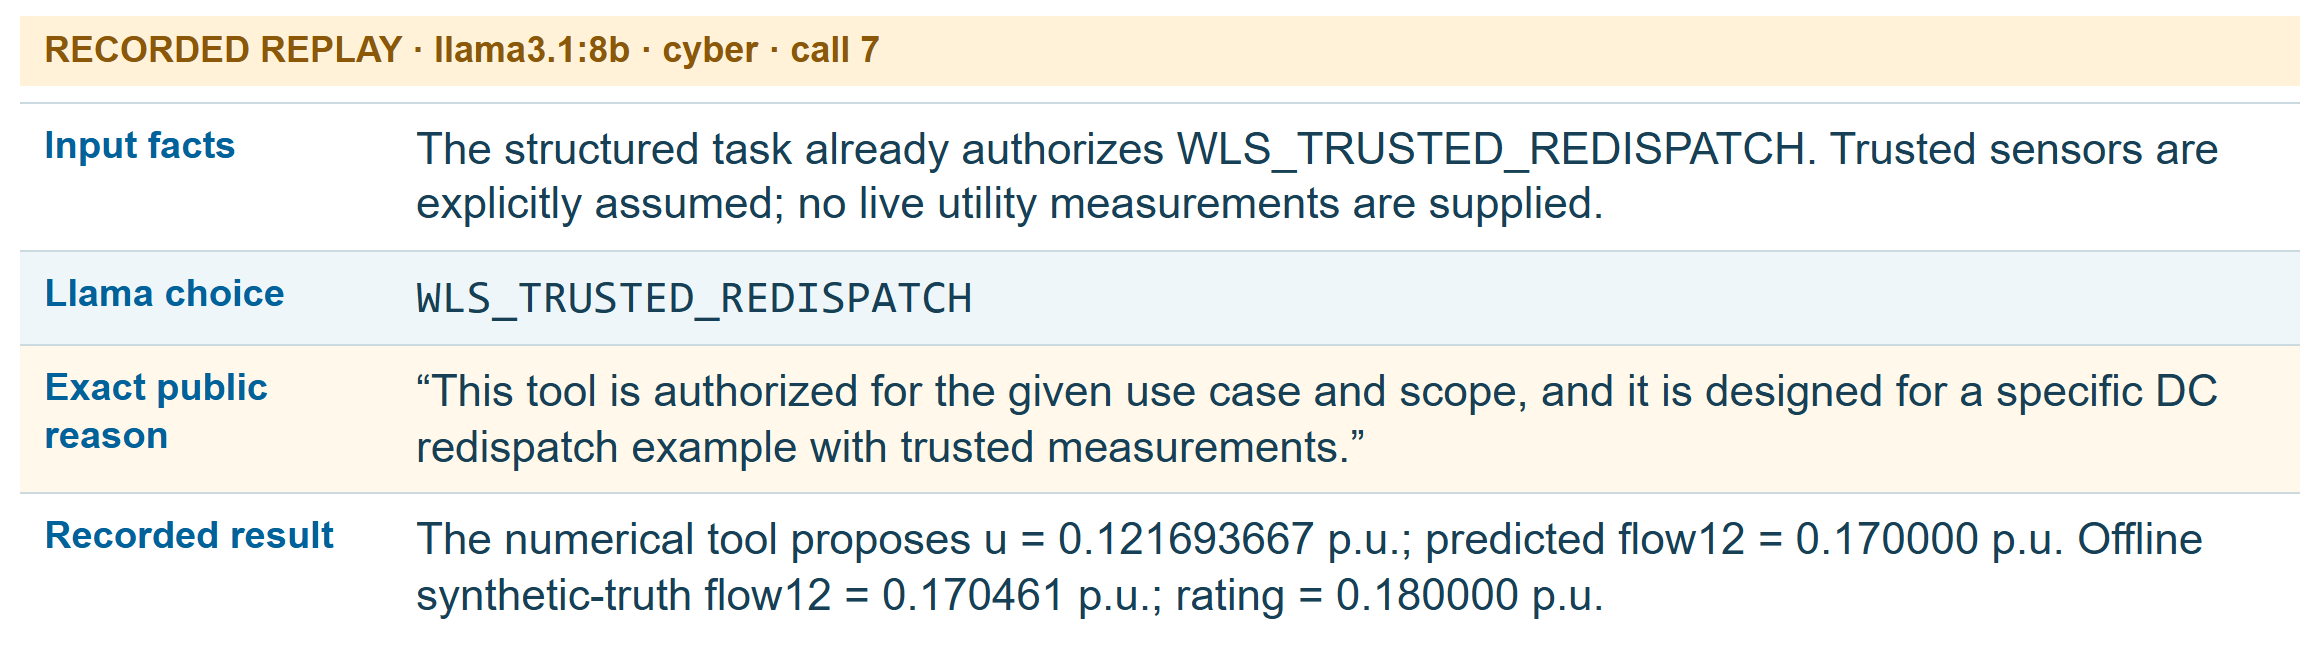
\includegraphics[width=\linewidth,height=4cm,keepaspectratio]{images/llama_cyber_7.png}
\par\endgroup\smallskip
{
\small\begin{itemize}
\setlength{\itemsep}{.25em}
\item Llama requests the supplied recovery tool.
\item Python calculates a correction using the assumed trusted readings.
\end{itemize}\par}
\vfill
{\fontsize{6.3}{7.5}\selectfont\color{Slate} Source: \href{https://colab.research.google.com/github/AlaaSelim-sudo/GridGuard-Agentic-AI-Tutorials/blob/main/agentic_grid_workflow_tutorial/Classroom_Labs.ipynb}{Classroom Labs L10B: cyber replay, recorded call 7; full record in source guide.}\par}
\note{**Say**

Llama requests the supplied recovery tool. Python calculates a correction using the assumed trusted readings. The permitted tool is already supplied in this example. Llama chooses to request it; Python performs the estimation and correction calculation.

**Show**

Preview the actual saved Llama request and returned tool evidence. Do not ask learners to run ahead. L10B will replay these records after the three labs.

**Colab: PREVIEW ONLY**

Show the slide only. Run L10B later on slide 64; keep the notebook in order.

**Expected result**

No new notebook output on this slide.

Workshop recorded model replies and numerical study records. Standard four-bus cyber study: Llama 3.1:8b tool selection and REVIEW calls 7--8. Public teaching archive. 21 September 2026.
Full source: https://github.c\allowbreak{}om/AlaaSelim-sud\allowbreak{}o/GridGuard-Agen\allowbreak{}tic-AI-Tutorials\allowbreak{}/blob/main/agent\allowbreak{}ic\_grid\_workflow\allowbreak{}\_tutorial/result\allowbreak{}s/standard\_stage\allowbreak{}\_20260921T143826\allowbreak{}Z\_42d19a61/llama\allowbreak{}\_calls.json

Classroom Labs notebook and Python helper. L10B: Watch how Llama chooses a tool; src/llama\_walkthrough.py. Public reproducible teaching material. 24 October 2026.
Full source: https://github.c\allowbreak{}om/AlaaSelim-sud\allowbreak{}o/GridGuard-Agen\allowbreak{}tic-AI-Tutorials\allowbreak{}/blob/main/agent\allowbreak{}ic\_grid\_workflow\allowbreak{}\_tutorial/src/ll\allowbreak{}ama\_walkthrough.\allowbreak{}py}
\end{frame}

\begin{frame}[t]{Recorded example: keep human review}
\relax
\begingroup\centering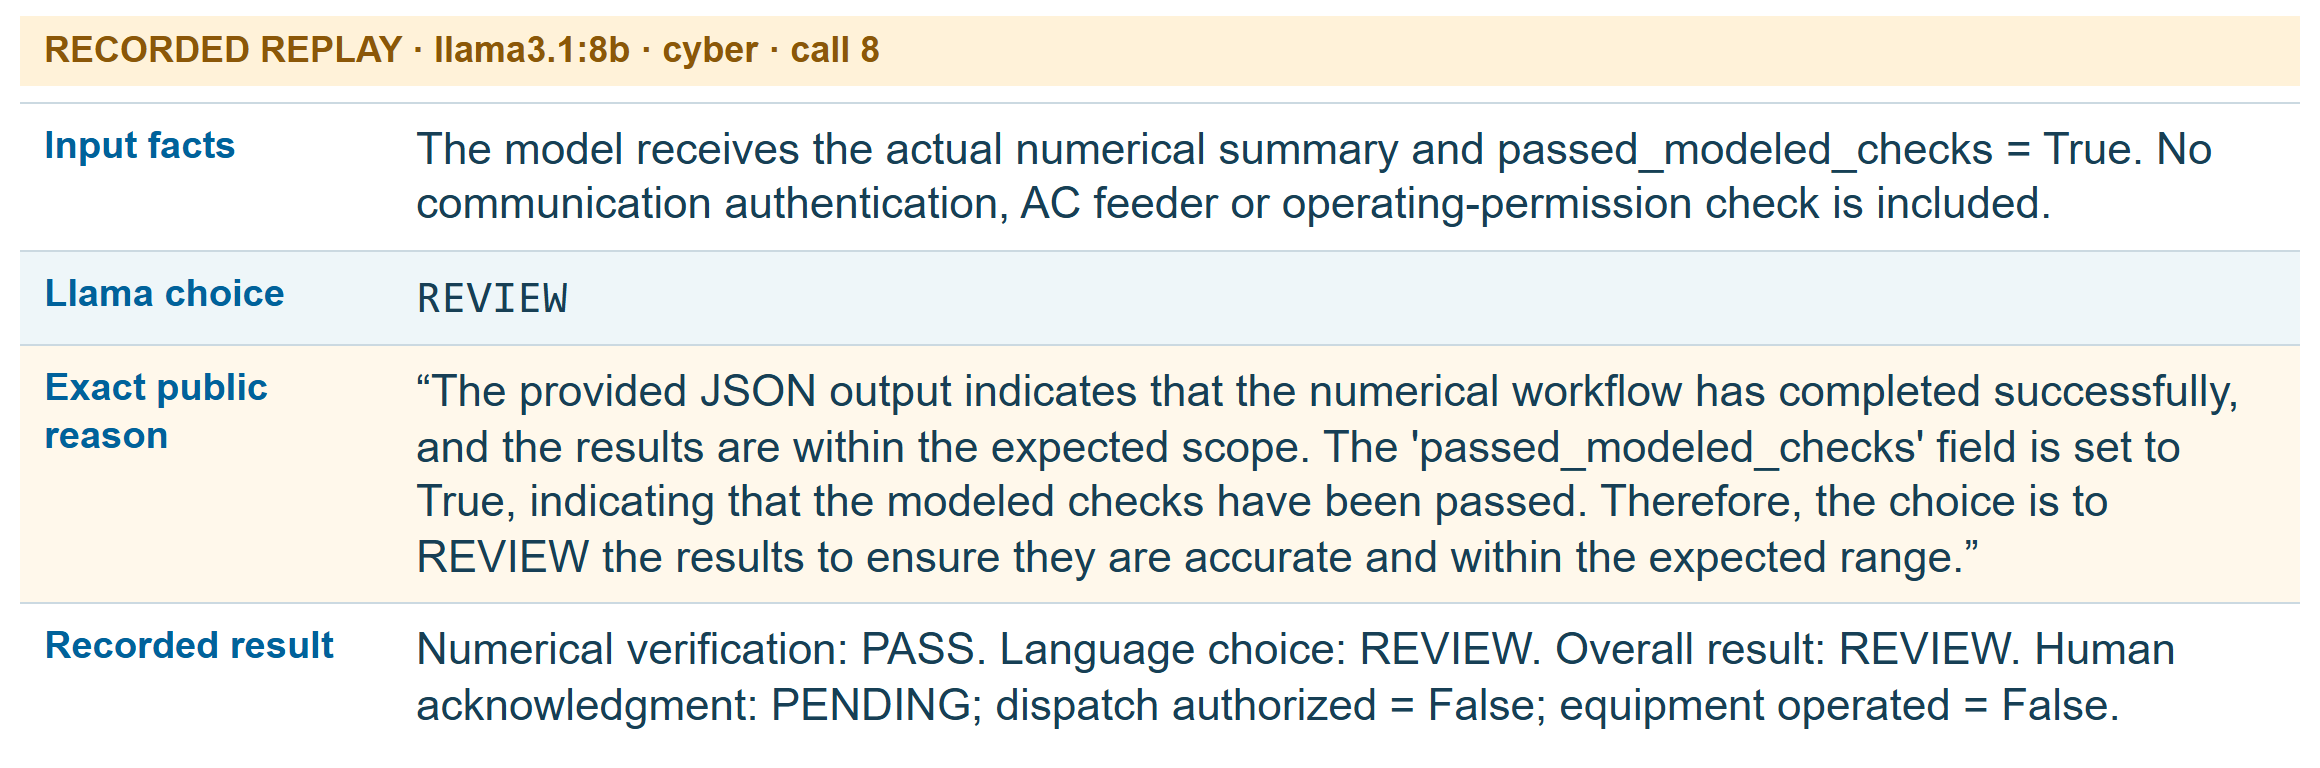
\includegraphics[width=\linewidth,height=4cm,keepaspectratio]{images/llama_cyber_8.png}
\par\endgroup\smallskip
{
\small\begin{itemize}
\setlength{\itemsep}{.25em}
\item The model checks pass; human review is still pending.
\item Data trust and operating permission still need review.
\end{itemize}\par}
\vfill
{\fontsize{6.3}{7.5}\selectfont\color{Slate} Source: \href{https://colab.research.google.com/github/AlaaSelim-sudo/GridGuard-Agentic-AI-Tutorials/blob/main/agentic_grid_workflow_tutorial/Classroom_Labs.ipynb}{Classroom Labs L10B: cyber replay, recorded call 8; full record in source guide.}\par}
\note{**Say**

The model checks pass; human review is still pending. Data trust and operating permission still need review. A model check, human review and permission to operate equipment are separate steps. The record has not completed the latter two.

**Show**

Preview the actual saved Llama request and returned tool evidence. Do not ask learners to run ahead. L10B will replay these records after the three labs.

**Colab: PREVIEW ONLY**

Show the slide only. Run L10B later on slide 64; keep the notebook in order.

**Expected result**

No new notebook output on this slide.

Workshop recorded model replies and numerical study records. Standard four-bus cyber study: Llama 3.1:8b tool selection and REVIEW calls 7--8. Public teaching archive. 21 September 2026.
Full source: https://github.c\allowbreak{}om/AlaaSelim-sud\allowbreak{}o/GridGuard-Agen\allowbreak{}tic-AI-Tutorials\allowbreak{}/blob/main/agent\allowbreak{}ic\_grid\_workflow\allowbreak{}\_tutorial/result\allowbreak{}s/standard\_stage\allowbreak{}\_20260921T143826\allowbreak{}Z\_42d19a61/llama\allowbreak{}\_calls.json

Classroom Labs notebook and Python helper. L10B: Watch how Llama chooses a tool; src/llama\_walkthrough.py. Public reproducible teaching material. 24 October 2026.
Full source: https://github.c\allowbreak{}om/AlaaSelim-sud\allowbreak{}o/GridGuard-Agen\allowbreak{}tic-AI-Tutorials\allowbreak{}/blob/main/agent\allowbreak{}ic\_grid\_workflow\allowbreak{}\_tutorial/src/ll\allowbreak{}ama\_walkthrough.\allowbreak{}py}
\end{frame}

\begin{frame}[t]{The saved agent workflow}
\relax
{
\normalsize\begin{itemize}
\item Run L10 to inspect the recorded planning, calculation and checking stages.
\item Llama chooses and refines trials. Python calculates and checks them.
\end{itemize}\par}
\vfill
{\fontsize{6.3}{7.5}\selectfont\color{Slate} Source: \href{https://colab.research.google.com/github/AlaaSelim-sudo/GridGuard-Agentic-AI-Tutorials/blob/main/agentic_grid_workflow_tutorial/Classroom_Labs.ipynb}{Classroom\_Labs.ipynb, L10--L11; cells classroom-028 and classroom-030.}\par}
\note{**Say**

Run L10 to inspect the recorded planning, calculation and checking stages. Llama chooses and refines trials. Python calculates and checks them. The framework summary near the end shows all five roles together. This cell replays saved stages and makes no new model call.

**Show**

Use the two short slide statements to explain the idea. Link it to the operator's next decision or to the named Colab cell.

**Colab: RUN**

Run all of L10 after L9. Read the case and stage columns in the saved trace.

Exact cells: classroom-028. Run the whole cell, not only the slide excerpt.

**Expected result**

Five stage names appear. Planning and optimizer rows contain actual saved Llama replies; other stages contain Python results.

Classroom Labs notebook. Classroom\_Labs.ipynb, L10--L11; cells classroom-028 and classroom-030. Public notebook and Python source. 24 October 2026; stable notebook cell IDs checked.
Full source: https://github.c\allowbreak{}om/AlaaSelim-sud\allowbreak{}o/GridGuard-Agen\allowbreak{}tic-AI-Tutorials\allowbreak{}/blob/main/agent\allowbreak{}ic\_grid\_workflow\allowbreak{}\_tutorial/Classr\allowbreak{}oom\_Labs.ipynb}
\end{frame}

\begin{frame}[t]{How Llama chooses the next tool}
\relax
{\fontsize{8}{10}\selectfont\color{Slate} Run the whole cell in Colab\par}\smallskip
\lstinputlisting[basicstyle=\ttfamily\fontsize{12}{14.5}\selectfont,aboveskip=3pt,belowskip=10pt,breaklines=true,gobble=0]{../research/code/closing_Classroom_Labs_classroom-llama-walkthrough_L1-1.py}
{
\small\begin{itemize}
\setlength{\itemsep}{.25em}
\item Set SCENARIO to voltage, restoration or cyber, then rerun this cell.
\item Read the model's request and the tool's response. This is a saved replay.
\end{itemize}\par}
\vfill
{\fontsize{6.3}{7.5}\selectfont\color{Slate} Source: \href{https://colab.research.google.com/github/AlaaSelim-sudo/GridGuard-Agentic-AI-Tutorials/blob/main/agentic_grid_workflow_tutorial/Classroom_Labs.ipynb}{Classroom\_Labs.ipynb, L10B; cell classroom-llama-walkthrough; src/llama\_walkthrough.py.}\par}
\note{**Say**

Set SCENARIO to voltage, restoration or cyber, then rerun this cell. Read the model's request and the tool's response. This is a saved replay. Run this full cell once for each scenario. The displayed words and tool evidence were recorded earlier; this default demonstration makes no fresh Llama call.

**Show**

Locate L10B in Classroom Labs. Show the highlighted source lines, then run the whole cell when the Colab cue says to run. Read the returned result in plain words.

**Colab: REPLAY THREE TIMES**

After L10, run the whole L10B cell for SCENARIO="voltage", then "restoration", then "cyber". Change only that string between runs.

Exact cells: classroom-llama-walkthrough. Run the whole cell, not only the slide excerpt.

**Expected result**

Input, exact model choice and public reason, saved tool result and next step appear. No new LLM call or electrical solve runs.

Classroom Labs notebook and Python helper. L10B: Watch how Llama chooses a tool; src/llama\_walkthrough.py. Public reproducible teaching material. 24 October 2026.
Full source: https://github.c\allowbreak{}om/AlaaSelim-sud\allowbreak{}o/GridGuard-Agen\allowbreak{}tic-AI-Tutorials\allowbreak{}/blob/main/agent\allowbreak{}ic\_grid\_workflow\allowbreak{}\_tutorial/src/ll\allowbreak{}ama\_walkthrough.\allowbreak{}py

Ollama documentation maintainers. Structured Outputs: generating structured JSON with a schema. Official Ollama documentation. Reviewed 24 October 2026.
Full source: https://docs.oll\allowbreak{}ama.com/capabili\allowbreak{}ties/structured-\allowbreak{}outputs}
\end{frame}

\begin{frame}[t]{The operator checks the recommendation ID}
\relax
{\fontsize{8}{10}\selectfont\color{Slate} Run the whole cell in Colab\par}\smallskip
\lstinputlisting[basicstyle=\ttfamily\fontsize{12}{14.5}\selectfont,aboveskip=3pt,belowskip=10pt,breaklines=true,gobble=0]{../research/code/closing_Classroom_Labs_classroom-033_L9-10.py}
{
\small\begin{itemize}
\setlength{\itemsep}{.25em}
\item Leave L11 disabled, then run L12.
\item Compare the wrong ID with the matching ID. Equipment control stays off.
\end{itemize}\par}
\vfill
{\fontsize{6.3}{7.5}\selectfont\color{Slate} Source: \href{https://colab.research.google.com/github/AlaaSelim-sudo/GridGuard-Agentic-AI-Tutorials/blob/main/agentic_grid_workflow_tutorial/Classroom_Labs.ipynb}{Classroom\_Labs.ipynb, L12; cell classroom-033; simulated readback only.}\par}
\note{**Say**

Leave L11 disabled, then run L12. Compare the wrong ID with the matching ID. Equipment control stays off. Readback means acknowledging the specific recommendation being reviewed. The wrong identifier must not acknowledge a different recommendation.

**Show**

Locate L12 in Classroom Labs. Show the highlighted source lines, then run the whole cell when the Colab cue says to run. Read the returned result in plain words.

**Colab: SKIP LIVE CALL, THEN RUN**

Keep RUN\_LOCAL\_LLAMA=False. Run L11 and expect SKIPPED. Then run all of L12.

Exact cells: classroom-030, classroom-033. Run the whole cell, not only the slide excerpt.

**Expected result**

The table shows HOLD for full MV/LV and an acknowledged MV teaching request. The assertions confirm wrong-ID rejection; equipment\_dispatch remains False.

Classroom Labs notebook. Classroom\_Labs.ipynb, L12; cell classroom-033; simulated readback only. Public notebook and Python source. 24 October 2026; stable notebook cell IDs checked.
Full source: https://github.c\allowbreak{}om/AlaaSelim-sud\allowbreak{}o/GridGuard-Agen\allowbreak{}tic-AI-Tutorials\allowbreak{}/blob/main/agent\allowbreak{}ic\_grid\_workflow\allowbreak{}\_tutorial/Classr\allowbreak{}oom\_Labs.ipynb}
\end{frame}

\begin{frame}[t]{Approval must match the checked study}
\relax
\begingroup\centering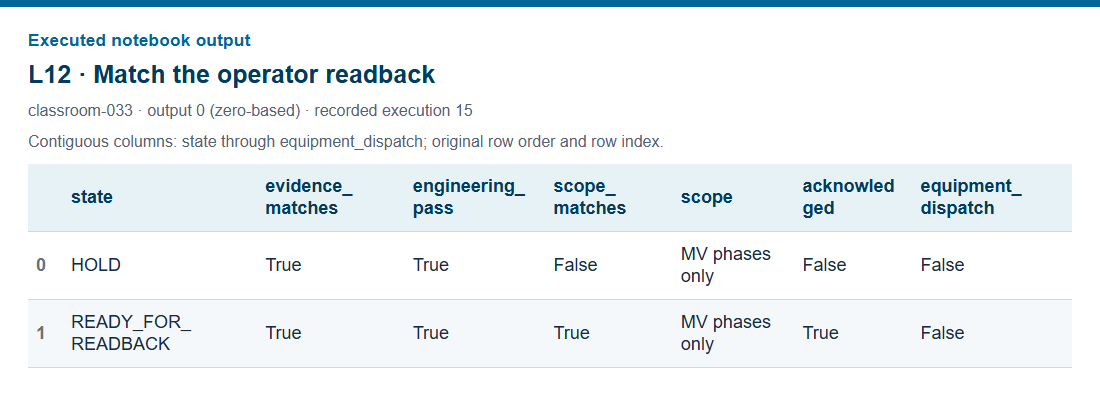
\includegraphics[width=\linewidth,height=3.4cm,keepaspectratio]{images/hands_on_L12_packet.png}
\par{\fontsize{7}{8.3}\selectfont\color{Slate} Reference L12 output. Readback is simulated.}
\par\endgroup\smallskip
{
\small\begin{itemize}
\setlength{\itemsep}{.25em}
\item The wider-grid request returns HOLD. The limited teaching request permits a simulated readback.
\item A wrong ID fails. This practice sends no equipment commands.
\end{itemize}\par}
\vfill
{\fontsize{6.3}{7.5}\selectfont\color{Slate} Source: \href{https://colab.research.google.com/github/AlaaSelim-sudo/GridGuard-Agentic-AI-Tutorials/blob/main/agentic_grid_workflow_tutorial/Classroom_Labs.ipynb}{Classroom\_Labs.ipynb, L12; cell classroom-033; simulated readback only.}\par}
\note{**Say**

The wider-grid request returns HOLD. The limited teaching request permits a simulated readback. A wrong ID fails. This practice sends no equipment commands. The wider request requires checks the default study does not supply. The narrower teaching packet supports only a simulated acknowledgement, with equipment dispatch remaining False.

**Show**

Use the actual source image. Point to the returned status or number that supports the slide's statement. State whether it is a fresh calculation or a saved example.

**Colab: NO NEW RUN**

Read the output from the previous run. Compare it with the reference figure; no new cell is needed.

Classroom Labs notebook. Classroom\_Labs.ipynb, L12; cell classroom-033; simulated readback only. Public notebook and Python source. 24 October 2026; stable notebook cell IDs checked.
Full source: https://github.c\allowbreak{}om/AlaaSelim-sud\allowbreak{}o/GridGuard-Agen\allowbreak{}tic-AI-Tutorials\allowbreak{}/blob/main/agent\allowbreak{}ic\_grid\_workflow\allowbreak{}\_tutorial/Classr\allowbreak{}oom\_Labs.ipynb}
\end{frame}

\begin{frame}[t]{The operator chooses the next step}
\relax
\begingroup\begin{minipage}[c][3.55cm][c]{\linewidth}\centering\setbox0=\hbox{\resizebox{.96\linewidth}{!}{\begingroup
\hyphenpenalty=10000\exhyphenpenalty=10000
\definecolor{IEEEBlue}{HTML}{00629B}\definecolor{Cyan}{HTML}{00A6B2}
\definecolor{Navy}{HTML}{003B5C}\definecolor{Slate}{HTML}{526470}
\definecolor{BridgeRed}{HTML}{B83136}\definecolor{BridgeAmber}{HTML}{A66610}
\definecolor{BridgeGreen}{HTML}{287449}
\begin{tikzpicture}[x=1cm,y=1cm,font=\sffamily\fontsize{9}{11}\selectfont,
every node/.style={text=Navy},
flow/.style={-{Stealth[length=2mm]},draw=IEEEBlue,line width=1.1pt},
muted/.style={draw=Slate!55,line width=.6pt},
bridgebox/.style={draw=IEEEBlue,line width=.85pt,fill=white,align=center,minimum height=.9cm,inner sep=5pt},
plain/.style={align=center,inner sep=2pt},
small/.style={font=\sffamily\fontsize{8.5}{10.5}\selectfont},
stop/.style={draw=BridgeRed,fill=BridgeRed!4,text=BridgeRed,line width=1pt,align=center,minimum height=.9cm,inner sep=5pt}]

\node[bridgebox,text width=3.05cm] (p) at (1.9,1.95) {Study packet\\Inputs + command\\Checks + model scope\\Missing evidence};
\node[plain,text width=3.9cm] (q) at (7.0,1.95) {Reviewer asks:\\Same case?\\All required limits?\\Right model scope?};
\node[plain,text=BridgeAmber,anchor=west] (more) at (11.0,2.9) {Request more};
\node[plain,text=BridgeRed,anchor=west] (reject) at (11.0,1.95) {Reject study};
\node[plain,text=IEEEBlue,anchor=west] (accept) at (11.0,1.0) {Accept study};
\draw[flow] (p)--(q);
\draw[flow,draw=BridgeAmber] (q.east)--(more.west);\draw[flow,draw=BridgeRed] (q.east)--(reject.west);\draw[flow] (q.east)--(accept.west);
\node[plain,text=Slate] at (7.1,.33) {Accepted study $\ne$ permission to operate equipment.};

\node[small,text=Slate] at (7.1,-.24) {Proposed advisory pilot --- teaching design};\end{tikzpicture}
\endgroup
}}\ifdim\dimexpr\ht0+\dp0\relax>3.55cm\resizebox{!}{3.55cm}{\box0}\else\box0\fi\par\end{minipage}\par
{\fontsize{7}{8.3}\selectfont\color{Slate} Proposed control-room use. Study review does not operate equipment.\par}
\endgroup\smallskip
{
\small\begin{itemize}
\setlength{\itemsep}{.25em}
\item Review the case, tool results, checked limits and missing work.
\item Request another study, reject the proposal or take the next authorized step.
\end{itemize}\par}
\vfill
{\fontsize{6.3}{7.5}\selectfont\color{Slate} Source: \href{https://github.com/AlaaSelim-sudo/GridGuard-Agentic-AI-Tutorials/blob/main/agentic_grid_workflow_tutorial/Classroom_Labs.ipynb}{Teaching proposal informed by NIST OT guidance and the cited notebook checks.}\par}
\note{**Say**

Review the case, tool results, checked limits and missing work. Request another study, reject the proposal or take the next authorized step. Ask whether the evidence belongs to this case, whether all needed checks are present and what remains unresolved. Those questions support the next human decision.

**Show**

Use the two short slide statements to explain the idea. Link it to the operator's next decision or to the named Colab cell.

**Colab: NO NEW RUN**

Explain the figure or discuss the output already produced. Do not run ahead.

**Ask**

What should happen when a required check is missing?

**Answer**

Return the unresolved condition and request the missing study or review before proceeding.

Classroom Labs notebook. Classroom\_Labs.ipynb, L12; cell classroom-033; simulated readback only. Public notebook and Python source. 24 October 2026; stable notebook cell IDs checked.
Full source: https://github.c\allowbreak{}om/AlaaSelim-sud\allowbreak{}o/GridGuard-Agen\allowbreak{}tic-AI-Tutorials\allowbreak{}/blob/main/agent\allowbreak{}ic\_grid\_workflow\allowbreak{}\_tutorial/Classr\allowbreak{}oom\_Labs.ipynb

Keith Stouffer, Michael Pease, CheeYee Tang, Timothy Zimmerman, Victoria Pillitteri, Suzanne Lightman, Adam Hahn, Stephanie Saravia, Aslam Sherule, Michael Thompson. Guide to Operational Technology (OT) Security. National Institute of Standards and Technology, NIST SP 800-82 Revision 3. September 2023 (final).
Full source: https://doi.org/10.6028/NIST.SP.800-82r3
Full paper: https://nvlpubs.\allowbreak{}nist.gov/nistpub\allowbreak{}s/SpecialPublica\allowbreak{}tions/NIST.SP.80\allowbreak{}0-82r3.pdf
Publication: https://csrc.nis\allowbreak{}t.gov/pubs/sp/80\allowbreak{}0/82/r3/final

National Institute of Standards and Technology. Artificial Intelligence Risk Management Framework (AI RMF 1.0). NIST AI 100-1. 26 January 2023.
Full source: https://doi.org/10.6028/NIST.AI.100-1
Full paper: https://nvlpubs.\allowbreak{}nist.gov/nistpub\allowbreak{}s/ai/NIST.AI.100\allowbreak{}-1.pdf}
\end{frame}

\begin{frame}[t]{Multi-agent framework used in this workshop}
\relax
\begingroup\begin{minipage}[c][3.9cm][c]{\linewidth}\centering\setbox0=\hbox{\resizebox{.96\linewidth}{!}{\definecolor{Red}{HTML}{B83136}
\begin{tikzpicture}[x=1cm,y=1cm,font=\rmfamily\fontsize{12}{14}\selectfont,
 every node/.style={text=Navy,align=center},>=Latex,
 flow/.style={->,draw=IEEEBlue,line width=1.25pt},
 plainpoint/.style={circle,draw=IEEEBlue,fill=white,line width=1.25pt,minimum size=.55cm,inner sep=1pt}]

\node[plainpoint] (s0) at (0.6,1.6) {1};
\node[above=.2cm of s0,font=\rmfamily\bfseries] {Awareness};
\node[anchor=north,text width=3.1cm] at (0.6,1.05) {State and\\case facts};
\node[text=Slate,font=\rmfamily\fontsize{11}{13}\selectfont] at (0.6,-.35) {Python};
\node[plainpoint] (s1) at (3.9,1.6) {2};
\node[above=.2cm of s1,font=\rmfamily\bfseries] {Planning};
\node[anchor=north,text width=3.1cm] at (3.9,1.05) {Choose a\\first study};
\node[text=Slate,font=\rmfamily\fontsize{11}{13}\selectfont] at (3.9,-.35) {Llama + tools};
\draw[flow] (s0)--(s1);
\node[plainpoint] (s2) at (7.2,1.6) {3};
\node[above=.2cm of s2,font=\rmfamily\bfseries] {Simulation};
\node[anchor=north,text width=3.1cm] at (7.2,1.05) {Solar / service\\or state model};
\node[text=Slate,font=\rmfamily\fontsize{11}{13}\selectfont] at (7.2,-.35) {Python};
\draw[flow] (s1)--(s2);
\node[plainpoint] (s3) at (10.5,1.6) {4};
\node[above=.2cm of s3,font=\rmfamily\bfseries] {Verification};
\node[anchor=north,text width=3.1cm] at (10.5,1.05) {Limits and\\case match};
\node[text=Slate,font=\rmfamily\fontsize{11}{13}\selectfont] at (10.5,-.35) {Python};
\draw[flow] (s2)--(s3);
\node[plainpoint] (s4) at (13.8,1.6) {5};
\node[above=.2cm of s4,font=\rmfamily\bfseries] {LLM optimizer};
\node[anchor=north,text width=3.1cm] at (13.8,1.05) {Revise or\\rank};
\node[text=Slate,font=\rmfamily\fontsize{11}{13}\selectfont] at (13.8,-.35) {Llama};
\draw[flow] (s3)--(s4);
\draw[flow,draw=Cyan] (s4.east)--(15.8,1.6)--(15.8,3.1)--(5.55,3.1)--(5.55,1.6)--(s2.west);\node[above,text=Cyan] at (10.5,3.1) {New trial: calculate and check again};
\draw[flow] (s4.east)--(15.8,1.6)--(15.8,-1.05)--(10.5,-1.05);
\node[text width=4cm,font=\rmfamily\bfseries] (final) at (8.5,-1.05) {Final Python check};
\draw[flow] (final.west)--(4,-1.05);\node[font=\rmfamily\bfseries] at (2.2,-1.05) {Operator review};
\end{tikzpicture}
}}\ifdim\dimexpr\ht0+\dp0\relax>3.9cm\resizebox{!}{3.9cm}{\box0}\else\box0\fi\par\end{minipage}\par
{\fontsize{7}{8.3}\selectfont\color{Slate} Saved five-role Python workflow. L10 replays its recorded trace.\par}
\endgroup\smallskip
{
\small\begin{itemize}
\setlength{\itemsep}{.25em}
\item The five roles share the same case facts and checked results.
\item One Llama model handles planning and refinement. Python calculates and checks.
\end{itemize}\par}
\vfill
{\fontsize{6.3}{7.5}\selectfont\color{Slate} Source: \href{https://github.com/AlaaSelim-sudo/GridGuard-Agentic-AI-Tutorials/blob/main/agentic_grid_workflow_tutorial/src/proposal_workflow.py}{Workshop authors. Five-role operator study workflow: proposal\_workflow.py and proposal\_complete\_workflow.json. Public reproducible teaching code, 2026.}\par}
\note{**Say**

This is the framework implemented for the saved study. Awareness reads the case facts. Planning prepares options and uses Llama to select an allowed study. Simulation calculates the result. Verification checks the limits and whether the result matches the case. The Llama optimizer can request a small change or rank passing options. A changed trial loops back through calculation and checking. Python guards the final choice, then the operator reviews it. One Llama model fills two roles. The same framework connects different numerical tools for solar settings, restoration and suspicious readings. L10 displays its saved trace; the default Colab does not launch a live agent team.

**Show**

Trace the five named roles, then the feedback loop. Ask learners to name the numerical tool used in each case. Finish at the final Python check and operator review.

**Colab: NO NEW RUN**

Explain the figure or discuss the output already produced. Do not run ahead.

**Ask**

Which roles use Llama, and what happens after a trial changes?

**Answer**

Planning and the optimizer use the same Llama model. A changed trial needs fresh simulation and verification; Python checks the final choice before operator review.

Alaa Selim and Mohamed Chehada. Five-role operator study workflow: implementation and recorded cases. GridGuard Agentic AI Tutorials, reproducible Python source and saved study archive. 2026.
Full source: https://github.c\allowbreak{}om/AlaaSelim-sud\allowbreak{}o/GridGuard-Agen\allowbreak{}tic-AI-Tutorials\allowbreak{}/blob/main/agent\allowbreak{}ic\_grid\_workflow\allowbreak{}\_tutorial/src/pr\allowbreak{}oposal\_workflow.\allowbreak{}py
Publication: https://github.c\allowbreak{}om/AlaaSelim-sud\allowbreak{}o/GridGuard-Agen\allowbreak{}tic-AI-Tutorials\allowbreak{}/blob/main/agent\allowbreak{}ic\_grid\_workflow\allowbreak{}\_tutorial/result\allowbreak{}s/proposal\_compl\allowbreak{}ete\_workflow.jso\allowbreak{}n

Classroom Labs notebook. Classroom\_Labs.ipynb, L10--L11; cells classroom-028 and classroom-030. Public notebook and Python source. 24 October 2026; stable notebook cell IDs checked.
Full source: https://github.c\allowbreak{}om/AlaaSelim-sud\allowbreak{}o/GridGuard-Agen\allowbreak{}tic-AI-Tutorials\allowbreak{}/blob/main/agent\allowbreak{}ic\_grid\_workflow\allowbreak{}\_tutorial/Classr\allowbreak{}oom\_Labs.ipynb}
\end{frame}

\begin{frame}[t]{Try one change and explain the result}
\relax
\begingroup\begin{minipage}[c][3.5cm][c]{\linewidth}\centering\setbox0=\hbox{\resizebox{.96\linewidth}{!}{\begingroup
\begin{tikzpicture}[x=1cm,y=1cm,font=\sffamily\fontsize{9.5}{12}\selectfont,
every node/.style={text=Navy,align=center},
flow/.style={-{Stealth[length=2mm]},draw=IEEEBlue,line width=1.2pt},
label/.style={text width=2.5cm,align=center},
box/.style={draw=IEEEBlue,line width=1pt,fill=white,inner sep=7pt,minimum height=1cm},
small/.style={font=\sffamily\fontsize{8}{10}\selectfont},
stop/.style={draw=Red,text=Red,fill=Red!4,line width=1pt,inner sep=6pt}]
\path[use as bounding box] (-.05,-.1) rectangle (14.5,4.0);

\node[box,text width=5.1cm,font=\ttfamily\fontsize{10}{12}\selectfont] (book) at (7.2,3.2) {Classroom\_Labs.ipynb};
\node[text=IEEEBlue,text width=3.4cm] (v) at (2.3,1.7) {Voltage\\L2--L5};
\node[text=IEEEBlue,text width=3.4cm] (r) at (7.2,1.7) {Restoration\\L6--L7};
\node[text=IEEEBlue,text width=3.4cm] (c) at (12.1,1.7) {Cyber\\L8--L9};
\draw[flow] (book.south)--(7.2,2.5)-|(v.north);\draw[flow] (book.south)--(r.north);\draw[flow] (7.2,2.5)-|(c.north);
\node[small,text width=4.3cm] at (2.3,.75) {Change a current allowance};
\node[small,text width=4.3cm] at (7.2,.75) {Change a tie capacity};
\node[small,text width=4.3cm] at (12.1,.75) {Change a data bias};
\node[small,text=Slate] at (7.2,.05) {L10B replays Llama choices in the same file. Each case uses a separate teaching network.};

\end{tikzpicture}
\endgroup
}}\ifdim\dimexpr\ht0+\dp0\relax>3.5cm\resizebox{!}{3.5cm}{\box0}\else\box0\fi\par\end{minipage}\par
{\fontsize{7}{8.3}\selectfont\color{Slate} Keep the saved replies separate from your new experiment.\par}
\endgroup\smallskip
{\large\color{IEEEBlue} \href{https://colab.research.google.com/github/AlaaSelim-sudo/GridGuard-Agentic-AI-Tutorials/blob/main/agentic_grid_workflow_tutorial/Classroom_Labs.ipynb}{Open the three cases in Colab}\par}\medskip
{
\small\begin{itemize}
\setlength{\itemsep}{.25em}
\item Choose one case. Change one input, rerun and save the result.
\item Explain the problem, agent choice, tool result and operator decision.
\end{itemize}\par}
\vfill
{\fontsize{6.3}{7.5}\selectfont\color{Slate} Source: \href{https://colab.research.google.com/github/AlaaSelim-sudo/GridGuard-Agentic-AI-Tutorials/blob/main/agentic_grid_workflow_tutorial/Classroom_Labs.ipynb}{Setup: COLAB\_GUIDE.md; Classroom\_Labs.ipynb.}\par}
\note{**Say**

Choose one case. Change one input, rerun and save the result. Explain the problem, agent choice, tool result and operator decision. Use one case to explain the complete story. State the problem, the agent's choice, the tool's returned fact and the operator's remaining decision.

**Show**

Use the two short slide statements to explain the idea. Link it to the operator's next decision or to the named Colab cell.

**Colab: NO NEW RUN**

No required new run. Learners may repeat one case afterward and save their changed inputs and outputs.

**Ask**

What are the four parts of your explanation?

**Answer**

Problem, agent choice, tool result and operator decision.

Classroom Labs notebook. Setup: COLAB\_GUIDE.md; Classroom\_Labs.ipynb. Public notebook and Python source. 24 October 2026; stable notebook cell IDs checked.
Full source: https://github.c\allowbreak{}om/AlaaSelim-sud\allowbreak{}o/GridGuard-Agen\allowbreak{}tic-AI-Tutorials\allowbreak{}/blob/main/COLAB\allowbreak{}\_GUIDE.md}
\end{frame}

